
\documentclass{ucbthesis}
\usepackage[backend=bibtex]{biblatex}

\usepackage[normalem]{ulem}

\usepackage{graphicx}
\usepackage{fancybox}
\usepackage{pseudocode}
%\usepackage{subfigure}
%\usepackage{cite}
\usepackage{xspace}
\usepackage{siunitx}
\usepackage{listings}


% Useful macros

\newcommand{\note}[1]{{\bf [ NOTE: #1 ]}}
\newcommand{\fixme}[1]{{\bf [ FIXME: #1 ]}}
\newcommand{\wunits}[2]{\mbox{#1\,#2}}
\newcommand{\um}{\mbox{$\mu$m}}
\newcommand{\xum}[1]{\wunits{#1}{\um}}
\newcommand{\by}[2]{\mbox{#1$\times$#2}}
\newcommand{\fix}[1]{\textcolor{red}{\bf #1}}
\def\eg{{\emph{e.g., }}}
\def\ie{{\emph{i.e., }}}

\newcommand{\todo}[1]{\noindent\textcolor{red}{[\underline{TODO}: #1]}}

\newcommand{\tess}{Tessellation\xspace}
%\newcommand{\tess}{MOS\xspace}
\newcommand{\pacora}{PACORA\xspace}
%\newcommand{\pacora}{ORADIA\xspace}

\newcommand{\BEAS}{\begin{eqnarray*}}
\newcommand{\EEAS}{\end{eqnarray*}}
\newcommand{\BEQ}{\begin{equation}}
\newcommand{\EEQ}{\end{equation}}
\newcommand{\BIT}{\begin{itemize}}
\newcommand{\EIT}{\end{itemize}}

\newcommand{\ones}{\mathbf 1}
\newcommand{\reals}{{\mbox{\textbf{R}}}}

\newcommand{\diag}{\mathop{\textbf{diag}}}
\newcommand{\argmin}{\mathop{\mathrm{argmin}}}
\newcommand{\argmax}{\mathop{\mathrm{argmax}}}

% Double spacing, if you want it.
% \def\dsp{\def\baselinestretch{2.0}\large\normalsize}
% \dsp

% If the Grad. Division insists that the first paragraph of a section
% be indented (like the others), then include this line:
% \usepackage{indentfirst}

\newtheorem{theorem}{Jibberish}

\bibliography{references}

\hyphenation{mar-gin-al-ia}

\begin{document}

% Declarations for Front Matter

\title{Optimizing Resource Allocations for Dynamic Interactive Applications}
\author{Sarah Bird}
\degreesemester{Spring}
\degreeyear{2014}
\degree{Doctor of Philosophy}
\cochairs{Professor Krste Asanovic}{Professor David Patterson}
\othermembers{Doctor Burton Smith \\
  Professor David Wessel}
\numberofmembers{4}
\prevdegrees{B.S. (University of Texas at Austin) 2007 \\
  M.S. (University of California, Berkeley) 2010}
\field{Computer Science}
\campus{Berkeley}


\maketitle
\approvalpage
\copyrightpage

\begin{abstract}
\fix{rewrite duplicate sentences}

Modern computing systems are under intense pressure to provide guaranteed responsiveness to their workloads.  Ideally, applications with strict performance requirements should be given just enough resources to meet these requirements consistently, without unnecessarily siphoning resources from other applications. However, executing multiple parallel, real-time applications while satisfying QoS requirements is a complex optimization problem and traditionally operating systems have provided little support to provide QoS to applications.  As a result, client, cloud and embedded systems have all resorted to over-provisioning and isolating applications to guarantee responsiveness.  We present \pacora, a resource allocation framework, which is designed to provide responsiveness guarantees to a simultaneous mix of high-throughput parallel, interactive, and real-time applications in an efficient, scalable manner.  By measuring application behavior directly and using convex optimization techniques,  \pacora is able to understand the resource requirements of applications and performance near optimal resource allocation with low overhead. 

\end{abstract}



\begin{frontmatter}

\begin{dedication}
\null\vfil
\begin{center}
To ???\\\vspace{12pt}
and why??
\end{center}
\vfil\null
\end{dedication}

\tableofcontents
\clearpage
\listoffigures
\clearpage
\listoftables

\begin{acknowledgements}
I want to thank my advisor for advising me.
\end{acknowledgements}

\end{frontmatter}

\pagestyle{headings}

% (Optional) \part{First Part}

\chapter{Introduction}

\chapter{Related Work}

\section{Related Work}\label{related_work}
\subsection{Batch Scheduling and Cluster Management}
Classic resource management systems were designed for batch scheduling~\cite{Feit97,FRS04}. Like \pacora, batch scheduling systems can allocate multiple resource types and rely on a gang-scheduling model~\cite{FeRu92}.  However, they tend to use queues and priorities to schedule jobs while trying to keep all resources busy. Resource allocations are always the user's responsibility to specify and pay for. Responsiveness can be improved by buying a higher priority. Few batch systems incorporate deadlines, but one such is \cite{AKKMS95}.

Modern cluster resource management has a similar flavor.  In systems such as
Amazon EC2~\cite{EC2}, Eucalyptus~\cite{eucalyptus}, and Condor~\cite{Condor}, users must specify their resource requirements.  Other systems such as Hadoop ~\cite{hadoop_fair, hadoop_cap, hadoop_matei} and Quincy~\cite{Quincy} use a fairness policy to assign resources. Mesos~\cite{mesos} uses two-level scheduling to manage resources in a cluster. Mesos decides how many resources to offer to its applications; they decide which resources to accept and how to schedule them. Mesos does not provide a particular resource allocation policy, but is a framework that can support multiple policies. Dominant Resource Fairness~\cite{mesos-DRF}, a generalization of max-min fairness to multiple resources types, has been implemented in Mesos.

\subsection{Model-Based Scheduling and Allocation Frameworks for SLAs and Soft Real-Time Requirements}

Research is growing in the cloud computing and realtime communities, which use application-specific performance ``models'' to try to schedule to meet deadlines or SLAs.

Much of this research has been in autonomic computing~\cite{1078472,1078493,1285843,1345325}. Typically, the performance models are utility functions derived from off-line measurements of raw resources utilization. These functions are either interpolations from tables or analytic functions based on queueing theory.
%The utility functions typically map the number of servers each execution environment receives to its performance relative to its requirements, which may be several.
A central arbiter maximizes total utility. The utility functions are not necessarily concave,
so the arbiter must use reinforcement learning or combinatorial search to make allocations.
%Each application has a manager that schedules the resources given to it by the arbiter.
Walsh \emph{et al.}\cite{1078411} note the importance of basing utility functions
on the metrics in which QoS is expressed rather than on the raw quantities of resources.
There are other philosophical similarities to \pacora, but since the objective functions are discrete and non-convex their optimization is difficult. A survey of autonomic systems research appears in \cite{1380585}.

Rajkumar \emph{et al.}\cite{828990} propose a system Q-RAM that maximizes the weighted sum of utility functions, each of which is a function of the resource allocation to the associated application. Unlike \pacora, there is no distinction between performance and utility, and the utility functions are assumed as input rather than being discovered by the system. The functions are sometimes concave, and in these cases the optimal allocation is easily found by a form of gradient ascent. When the utility functions are not concave, a suboptimal greedy algorithm is proposed.
%They are always nondecreasing in every resource and sometimes are piecewise-linear and concave;

Several systems use a feedback-driven reactive approach to resource allocation where a control loop or reinforcement learning adjusts allocations continuously. AcOS\cite{AcOS} and Metronome\cite{Metronome} feature hardware-thread based maintenance of ``heart rate'' targets using adaptive reinforcement learning.
%AcOS also senses thermal conditions and can exploit Dynamic Voltage and Frequency Scaling (DVFS).
Bodik \emph{et al.}\cite{bodik-acdc09} builds online performance models like \pacora.
Initially, it uses an \emph{exploration policy} that avoids nearly all SLA violations while it builds the model; later, it shifts to a controller based on the model it has built.
The models are statistical, and bootstrapping is used to estimate performance variance.
Major changes in the application model are detected and cause model exploration to resume.
%The models are not convex or concave in general, and all SLAs must be met with high probability.

Jockey\cite{Jockey} has some similarities to \pacora: it is intended to handle parallel computation, its utility functions are concave,
and it adapts dynamically to application behavior.
Its performance models are obtained by calibrating either event-based simulation or a version of Amdahl's Law to computations.
Jockey does not optimize total utility but simply increases processors until utility flattens for each application,
\emph{i.e.,} each deadline is met.
A fairly sophisticated control loop prevents oscillatory behavior.

Other systems base decisions on user-provided resource specifications and a real-time scheduling algorithm.  In the Redline system\cite{Redline}, compact resource requirement specifications written by hand to guarantee response times are scheduled Earliest-Deadline-First.
%Isolation of resources is strong, as in \pacora.  Scheduling is Earliest-Deadline-First.
%Admission control is lenient but oversubscription situations are remedied by de-admitting some of the non-interactive applications.

Much research focuses on measuring resource usage to make smart co-scheduling decisions.
For example, Calandrino \emph{et al.}\cite{unc} uses working set sizes to make co-scheduling decisions and enhance soft real-time behavior. Merkel and Bellosa\cite{merkel-eurosys08} propose \emph{Task Activity Vectors} that describe how much each application uses the various functional units; these vectors are used to balance usage across multiple cores.
%and unbalance usage among hardware threads within each core.
%The intended effect is to distribute chip temperature more evenly, but the idea may be more broadly applicable, \emph{e.g.,} for heterogeneous systems.

 Some frameworks can support multiple scheduling and resource allocation policies. Guo \emph{et al.}\cite{1331730} present such a framework.  They point out that much prior work is insufficient for true QoS; merely partitioning hardware is not enough because there must also be a way to specify performance targets and an admission control policy for jobs. Unlike \pacora, they argue that targets should be expressed in terms of capacity requirements rather than rates or times.

Nesbit \emph{et al.}\cite{1436097} introduces \emph{Virtual Private Machines} (VPM), a framework for resource allocation and management in multicore systems. A VPM comprises a set of virtual hardware resources, both spatial (physical allocations) and temporal (scheduled time-slices).
%They break down the framework components into policies and mechanisms which may be implemented in hardware or software.
VPM \emph{modeling} maps high-level application objectives via
\emph{translation}, which uses models to assign acceptable VPMs to
applications while adhering to system-level policies. A
\emph{scheduler} decides if the system can accommodate all
applications. The VPM approach and terminology are similar to
\pacora's at a high level, but no design or implementation of the
modeling, translation, or scheduling components is presented~\cite{1436097}.
%mesh well with our study, which can be seen as a specific implementation of several key aspects of the type of framework they describe (i.e. VPM modeling and translation).
%
%Unlike traditional virtual machines that only virtualize resource functionality, VPMs virtualize a system's performance and power characteristics, meaning that a VPM has the same performance and power profile as a real machine with an equivalent set of hardware resources.

\subsection{Resource Partitioning and QoS}
\label{sec:rel:pm}

\pacora relies on resource partitioning and Quality-of-Service mechanisms when available to enforce its resource allocation decisions.  Resource partitioning and QoS research is active for on-chip, cluster, and networking resources.  However, the vast majority of research focuses on allocating a single resource type with a fixed policy, typically \emph{fairness}.
Some have researched network bandwidth fairness~\cite{Blanquer, Kleinberg99fairnessin, Liu}, while others~\cite{Baruah96proportionateprogress, Baruah_fastscheduling, Zhu} have concentrated on CPU fairness.

Hardware partitioning research, which has largely focused on caches, provides mechanisms based on policies baked into the hardware, not the flexible allocations \pacora requires \cite{876484, 967444,1194855,1275005,1194858,1318096,1088154,1399973,1069998,1399982}.  Early work focused on providing adaptive, fair policies that ensure equal performance degradation \cite{605420,1086328}, not guarantees of responsiveness. More recent proposals have incorporated more sophisticated policy management \cite{1241608,1331730,1152161,1254886}. Iyer\cite{1006246} suggests a priority-based cache QoS framework, CQoS, for shared cache way-partitioning.
%The priorities might be specified per core, per application, per memory type, or even per memory reference.
However, simultaneous achievement of performance targets as in \pacora is not addressed.


%In general, these papers focus on designing and proving the effectiveness of particular mechanisms for particular goalswithout a concrete notion of a general-purpose resource allocation or scheduling framework.
%in which a variety of application-specific QoS requirements can be communicated to an all-purpose resource allocator and scheduler.



%The Singularity operating system\cite{aiken-mspc06} provides process isolation through software rather than hardware.  This isolation in accessibility is not the same as the performance isolation that is desirable for \pacora.

%Other partitioning work has focused on interconnect bandwidth QoS \cite{1382130} or partitioning cache capacity and bandwidth simultaneously \cite{1250671}.

%CQoS: a framework for enabling QoS in shared caches of CMP platforms
%\cite{1006246}

%Suh \emph{et al.}\cite{876484, 967444} and Qureshi and Patt \cite{1194855} monitor individual applications' cache performance to decide partitioning in an attempt to reduce the total amount of cache misses and off-chip memory traffic.
%A wide variety of proposals exist for multicore last-level cache structures that partition the spatial resources between private and shared data, in an attempt to create a manageable trade-off between capacity for shared data and low latency for private data \cite{1275005,1194858,1318096,1088154,1399973,1069998,1399982}.

%\subsection{Application Performance Modeling}
%
%\fix{add information here}


%Citations supporting PACORA's assumptions.

%Ganapathi \emph{et al.} have had success using machine learning to model application performance and select the best performing configuration in \cite{Archana}.

%Kumar \emph{et al.}\cite{1006707} demonstrate the performance advantages of heterogeneous cores for mixed workloads using heuristic allocation strategies in both space and time.
%
%Genbrugge and Eeckhout\cite{genbrugge-isca07} demonstrate the importance of adapting to changes in application characteristics, in this case instructions per cycle.

%\todo{I DON'T KNOW WHY \cite{975344,wasserman-book} ARE IN HERE}

%Scheduling threads for constructive cache sharing on CMPs
%\cite{1248396}
%
%Chen \emph{et al.}\cite{1248396} propose parallel depth-first thread scheduling as an alternative to work-stealing for constructive cache sharing.
%The paper discusses the automation of task granularity selection to match cache capacity. This kind of tuning is particularly appropriate for a user-level runtime system.


%\subsection{Autonomic Systems}
%Resource Allocation for Autonomic Data Centers using Analytic Performance Models
%	\cite{1078472}
%	
%Autonomic QoS-aware resource management in grid computing using online performance models
%	\cite{1345325}
%
%On the use of hybrid reinforcement learning for autonomic resource allocation
%\cite{1285843}
%	
%Utility-Function-Driven Resource Allocation in Autonomic Systems
%\cite{1078493}

%Redline: First Class Support for Interactivity in Commodity OSs \cite{Redline}
%Paper presented in OSDI'08.
%

%Jockey: Guaranteed Job Latency in Data Parallel Clusters \cite{Jockey}
%Work from Microsoft about the system they built on top of their Cosomos cluster (Dryad???)

%Discusses how they do the dynamic resource allocation for jobs running in a cluster
%Paper from Eurosys 2012
%


%Automatic Exploration of Datacenter Performance Regimes
%\cite{bodik-acdc09}
%

%AcOS: an Autonomic Management Layer Enhancing Commodity Operating Systems \cite{AcOS}
%Work at the Politecnico di Milano, Italy.
%Master Thesis
%Paper and slides at the CHANGE 2012 Workshop (DAC)
%
%Metronome: OS Level Performance Management via Self Adaptive Computing \cite{Metronome}
%Work related to AcOS, done by people from the Politecnico di Milano (Italy), MIT and Harvard.
%Paper presented in DAC 2012.

%A resource allocation model for QoS management
%\cite{828990}
%

%Utility-Based Cache Partitioning: A Low-Overhead, High-Performance, Runtime Mechanism to Partition Shared Caches
%\cite{1194855}
%


\chapter{PACORA Framework}
%------------------------------------------------------------------------------------------------------------------------------------------------------------------------
\section{Introduction}
%------------------------------------------------------------------------------------------------------------------------------------------------------------------------
\pacora is a framework designed to determine the proper amount of each
resource type to give each application.  The purpose of \pacora is to dynamically assign resources
across multiple applications to guarantee responsiveness without
over-provisioning and to adapt allocations as the application mix
changes. For example, consider a video conference scenario where each participant requires a separate,
performance-guaranteed video stream.  New participants may join the
conference and others may leave, increasing or decreasing the number
of streams running at any given time.  Simultaneously, participants
may be collaborating through web browsers, or watching shared video
clips and web searching, while their systems run compute-intensive
background tasks such as updates, virus scans, or file indexing.
Although it may be relatively straightforward to provide
responsiveness guarantees for individual applications such as video
streams, the real challenge is to do so without reserving excessive
resources, which will compromise system utilization, power
consumption, or responsiveness of other applications.

We believe \pacora is applicable to many resource-allocation
scenarios, from cloud providers determining how many resources to give
each job to avoid violating Service-Level Agreements (SLAs), through databases allocating
resources to queries, to distributed embedded systems allocating
bandwidth among devices and sensors.  These potential applications of \pacora are discussed in greater detail in Chapter~\ref{discuss}. In this chapter, we describe the mathematical formulation of the \pacora framework, prove the convexity, and present our initial evaluations of the potential of using \pacora for resource allocation in an operating system.

%------------------------------------------------------------------------------------------------------------------------------------------------------------------------
\section{\pacora Architecture}\label{sys_design}
%------------------------------------------------------------------------------------------------------------------------------------------------------------------------
\pacora formulates resource allocation as an optimization problem
built from two types of application-specific functions: a
response-time function and a penalty function. The response-time
function represents the performance of the application with different
resources and is built with runtime measurements.  The penalty
function represents the user-level goals for the application
(\emph{i.e.,} the deadline and how important it is to meet). \pacora uses convex optimization~\cite{BoVa} to
determine the ideal resource allocation across all active
applications.  The following subsections briefly introduce the primary
components of \pacora and the optimization formulation.

\subsection{Response-Time Functions}

Response-time functions (RTF) represent the expected \emph{response
  time} of an application as a function of the resources allocated to
the application. The response time is an application-specific measure
of the performance of the application.  For example, the response time
of an application might be:
    \begin{itemize}\itemsep0pt \parskip0pt \parsep5pt
    \item The time from a mouse click to its result;
    \item The time to produce a frame;
    \item The time from a service request to its response;
    \item The time from job launch to job completion;
    \item The time to execute a specified amount of work.
    \end{itemize}

The RTFs are built to be convex functions.  All applications have a
function of the same form, but the application-specific weights are set
using the performance history of the application.  RTFs are designed
to capture information such as how well an application scales with a
particular resource. As a result, RTFs naturally support
heterogeneity.  Each CPU or GPU type is simply viewed as a different
resource type by the system, and thus the RTFs will represent how
effectively an application uses a particular type of
core. Figure~\ref{sample_rtf} shows two example RTFs we have created
from applications we studied.

\begin{figure*}[hb]
\subfloat{
\includegraphics*[bb=0 0 360 360,width=.48\columnwidth]{Figures/bfs-fig.pdf}
\label{bfs-fig}
}
\subfloat{
\includegraphics*[bb=0 0 360
  360,width=.48\columnwidth]{Figures/streamcluster-fig.pdf}
\label{streamcluster-fig}
}  
\caption{\label{sample_rtf} Response-Time Functions for a
  breadth-first search algorithm and \texttt{streamcluster} from the PARSEC benchmark suite~\cite{parsec}. We show two resource dimensions: cores and cache ways.}
\end{figure*}

Equation~\ref{rtf_eq} below shows the RTF we selected for \pacora.  

\begin{equation}\label{rtf_eq}
\tau(w,a) = \tau_0 + \sum_{i\in n,j\in n}{\frac{w_{i,j}}{\sqrt{a_i * a_j}}}
\end{equation}

Here $\tau$ is the response time, $i$ and $j$ are
resource types, $n$ is the total number of resource types,
$a_{i}$ and $a_{j}$ are the allocations of resource types $i$
and $j$, and $w_{i,j}$ is the application-specific weight for
the term representing resources $i$ and $j$.

In our experience the cross term weights (those with $i\neq j$) are almost always negligible and can be omitted if desired.
This omission allows the dimensionality of the function, and thus the storage space required, to increase roughly linearly with the number of resource types.  The value of the cross terms is discussed further in Section~\ref{init_eval}.

We chose this specific function because it is convex in the resources, and in initial application studies,
we found it models response time behavior accurately enough to allow the optimization to make good decisions. Section~\ref{RTFs} describes the design considerations for the RTFs in more detail. Section~\ref{init_eval} shows these evaluation results and discusses alternative models that were considered and evaluated during the design process.

\subsection{Penalty Functions}

Penalty functions are designed to represent the user-level goals of
the application. They are similar to priorities but are functions of
the response time rather than simply values, so they can explicitly
represent deadlines.  Knowing the deadlines lets the system make
optimizations that are difficult in today's systems, such as running
just fast enough to make the deadline. Like priorities, the penalty
functions are set by the system on behalf of the user.


\begin{figure}[hb]
\parbox{3in}{
\includegraphics*[width=.45\columnwidth]{Figures/Penalty1.eps}
\caption{\label{f:pen1}A penalty function with a response time constraint.}
}
\hspace{\fill}
\parbox{3in}{
\includegraphics*[width=.45\columnwidth]{Figures/Penalty2.eps}
\caption{\label{f:pen2}A penalty function with no response time constraint.}
}
\end{figure}

\pacora's penalty functions $\pi$ are non-decreasing piecewise-linear
functions of the response time $\tau$ of the form $\pi(\tau) = \max(0, (\tau - d)s)$
where $d$ represents the deadline of the application and $s$ (slope)
defines the rate the penalty increases as response time increases. For
applications without response-time constraints the deadline can be set
to $0$. Two representative graphs of this type appear in
Figures~\ref{f:pen1} and~\ref{f:pen2}.

\subsection{Resource Allocation as Optimization}

\pacora formulates resource allocation as an optimization problem
designed to minimize the total penalty of the system. This approach is
analogous to minimizing user dissatisfaction with the user experience
due to missed deadlines in a client system and minimizing the contract
penalties paid for violated SLAs in a cloud
system.

The optimization selects the allocations for all resources and
resource types at once.  This approach enables the system to make
tradeoffs between resource types.  For example, the system could
choose to allocate more memory bandwidth in lieu of on-chip cache, or
one large core instead of several small cores.  Given that all of the
resources allocated to an application contribute to the response time,
it would difficult to provide predictable response times for
applications without over-provisioning by independently allocating each resource type.

A succinct mathematical characterization of this resource allocation scheme is the following:
\begin{eqnarray}
& \makebox[1in][r]{Minimize}   & \sum_{p\in P} {\pi_p(\tau_p(a_{p,1}\ldots a_{p,n}))}  \\
& \makebox[1in][r]{Subject to} & \sum_{p\in P} a_{p,r} \leq A_r, r = 1,\ldots n        \\
& \makebox[1in][r]{and}        & a_{p,r} \geq 0
\end{eqnarray}
Here $\pi_p$ is the penalty function for application $p$,
$\tau_p$ is its response time function,
$a_{p,r}$ is the allocation of resource $r$ to application $p$,
and $A_r$ is the total amount of resource $r$ available. 

\subsection{Managing Power and Energy}
In \pacora, we create an artificial application to represent the
interest in reducing the power and energy of the system.  Application 0 is
designated the idle application and receives allocations of all
resources that are left idle, \emph{i.e.,} not allocated to other
applications.  If the system has the appropriate power management mechanisms, these idle resources can be powered off or put to sleep to save power.

Additionally, application 0 functions as \emph{slack} variables in our optimization problem turning the resource bounds into equalities:
\begin{equation}
\sum_{p\in P} a_{p,r} - A_r = 0, r = 1,\dots n.
\end{equation}

The ``response time'' for application 0, $\tau_0$, is artificially
defined to be the total system power consumption.  Application 0's RTF represents how the system power improves when particular resources are left idle (\emph{i.e.,} allocated to application 0), which is similar to other RTFs since they represent how the response time of an application improves when allocated particular resource types. This response function is affine and monotone non-increasing in its arguments $a_{0,r}$.

The penalty function $\pi_0$ establishes a system tradeoff between
power and performance that will determine which resources are
allocated to applications to improve performance and which are left
idle.  The penalty function $\pi_0$ can be used to keep total system
power below the parameter $d_0$ to the extent the penalties of other
applications cannot overcome its penalty slope $s_0$. Both $s_0$ and
$d_0$ can be adjusted to reflect the current battery charge in mobile
devices. For example, as the battery depletes, $d_0$ could be decreased or $s_0$ increased
to force other applications to slow or cease execution.


%------------------------------------------------------------------------------------------------------------------------------------------------------------------------
\section{Convex Optimization}
%------------------------------------------------------------------------------------------------------------------------------------------------------------------------
If the penalty functions, response time functions, and resource
constraints were arbitrary, little could be done to optimize the total
penalty beyond searching at random for the best allocation.  However, we designed \pacora to be convex by construction, which enables us to use convex optimization~\cite{BoVa} methods to solve the optimization. 
By framing our resource allocation problem as a convex optimization problem, we get two significant benefits: for each problem an optimal
solution exists without multiple local extrema, and fast optimization methods with practical incremental solutions become feasible.  In this section, we prove the convexity of \pacora's optimization formulation and the penalty and RTF functions. \pacora also formulates RTF \emph{creation} as a convex optimization
problem, as explained in Section~\ref{rtf_creation}.

\subsection{Resource Allocation Optimization Convexity}

A constrained optimization problem is \emph{convex} if both the objective function to be minimized
and the constraint functions that define its feasible solutions are convex functions.
A function $f$ is convex if its domain is a convex set and
$f(\theta x + (1-\theta)y) \leq \theta f(x) + (1-\theta)f(y)$
for all $\theta$ between 0 and 1.
A set is convex if for any two points $x$ and $y$ in the set, the point
$\theta x + (1-\theta)y$
is also in the set for all $\theta$ between 0 and 1.
If $f$ is differentiable, it is convex if its domain is an open convex set and
$f(y) \geq f(x) + \nabla f^T\cdot(y-x)$ where $\nabla f$ is the gradient of $f$.
Put another way, $f$ is convex if its first-order Taylor approximations
are always global underestimates of its true value.

A convex optimization problem is one that can be expressed in this form:
\begin{eqnarray*}
& \makebox[1in][r]{Minimize}   & f_0(x_1,\ldots x_m)                              \\
& \makebox[1in][r]{Subject to} & f_i(x_1,\ldots f_m) \leq 0, i = 1,\ldots k        \\
& \makebox[1in][r]{where}      & \forall i \quad f_i:\Re^m \rightarrow \Re \mbox{ is convex.}
\end{eqnarray*}


\pacora's resource allocation problem can be transformed into a convex
optimization problem in the $m = |P|\cdot n$ variables $a_{p,r}$ as
long as the penalty functions $\pi_p$ are convex non-decreasing and
the response-time functions $\tau_p$ are convex.  We designed our
functions to meet these constraints, and proofs of their convexity are shown below.
 
The resource constraints are affine and therefore convex; they can be rewritten as 
\begin{equation}
\sum_{p\in P} (a_{p,r} - A_r) \leq 0  -a_{p,r} \leq 0
\end{equation}
\begin{equation}
-a_{p,r} \leq 0
\end{equation}

The convex formulation makes the optimization scale linearly in the
number of resource types and the number of applications.  For client
operating systems with around 100 applications running and 10 resource
dimensions, the total number of variables in the optimization problem
is 1000---a very small problem which is solved in microseconds on
current systems.  Cloud systems could have many more than 100
applications running, but the problem size scales linearly and the
potential benefits of a good allocation should scale rapidly with the
size of the system.

\subsection{Penalty Function Convexity}
In this section, we discuss the convexity of \pacora's penalty functions.
A few facts about convex functions will be useful in what follows.
First, a \emph{concave} function is one whose negative is convex.
Maximization of a concave function is equivalent to minimization of its convex negative.
An affine function, one whose graph is a straight line in two dimensions or a hyperplane in n dimensions,
is both convex and concave.  A non-negative weighted sum or point-wise maximum (minimum) of convex (concave) functions is convex (concave), as is either kind of function composed with an affine function.  The composition of a convex non-decreasing (concave non-increasing) scalar function with a convex function remains convex (concave).

Each penalty function $\pi$ is the pointwise maximum of two affine functions and is therefore convex.
Moreover, since each penalty function is scalar and nondecreasing,
its composition with a convex response time function will also be convex.

\subsection{Response Time Convexity}
We now show that response time functions $\tau$ including the various bandwidth amplification functions are convex
in both the bandwidth and memory resources $b_r$ and $m_r$ given any of the possibilities we have considered.
Since norms preserve convexity, this reduces the question to proving each term in the norm is convex.
Since all quantities are positive and both maximum and scaling by a positive constant preserve convexity,
\begin{eqnarray*}
\lefteqn{w/(b\cdot\min(c_1\alpha_1(m),c_2\alpha_2(m)))}   \\
&=& \max(w/(b\cdot c_1\alpha_1(m)),w/(b\cdot c_2\alpha_2(m))).
\end{eqnarray*}
It therefore only remains to show that both $1/\sqrt{b\cdot m}$ and $1/(b\cdot\alpha(m))$ are convex in $b$ and $m$.

A function is defined to be \emph{log-convex} if its logarithm is convex.
A log-convex function is itself convex because exponentiation preserves convexity,
and the product of log-convex functions is convex because the log of the product is the sum of the logs,
each of which is convex by hypothesis.
Now $1/b$ is log-convex for $b > 0$ because $-\log b$ is convex on that domain.
In a similar way, $\log(1/\sqrt{b\cdot m}) = -(\log b + \log m)/2$
and $\log m^{-1/d} = -(\log m)/d$ are convex.
Finally, $\log (1/\log m)$ is convex because its second derivative is positive for $m > 1$:
\begin{eqnarray*}
\frac{d^2}{dm^2}\log (1/\log m) &=& \frac{d^2}{dm^2}(-\log\log m)  \\
                                  &=& \frac{d}{dm}\left(\frac{-1}{m\log m}\right) \\
                                  &=& \frac{1 + \log m}{(m\log m)^2}.
\end{eqnarray*}

Summing up, a response time function for a application might be modeled by the convex function
\begin{eqnarray*}
\tau(w,b,\alpha,m) &=& \sqrt[p]{\sum_j \left(\frac{w_j}{b_j\cdot\alpha_j(m_j)}\right)^p}  \\
                   &=& \|\mbox{diag} wd^T \|_p
\end{eqnarray*}
where the $w_j$ are the parameters of the model (the quantities of work) to be learned,
the components of $d$ satisfy $d_j = 1/(b_j\cdot\alpha_j(m_j))$,
the $b_j$  are the allocations of the bandwidth resources,
the $\alpha_j$ are the bandwidth amplification functions (also to be learned),
the $m_j$ are the allocations of the memory or cache resources that are responsible for the amplifications.
This formulation allows the application response time $\tau$ to be modeled as the $p$-norm of
the component-wise product of a vector $d$ that is computed from the resource allocation
and a learned vector of work quantities $w$.


%------------------------------------------------------------------------------------------------------------------------------------------------------------------------
\section{Definitions and Assumptions}
%------------------------------------------------------------------------------------------------------------------------------------------------------------------------
In Section~\ref{sys_design}, we have presented the mathematical framework behind \pacora.  In this Section, we further define terms such as application and resource and describe the assumptions that \pacora makes about the system design in order to explain how the framework would operate to perform resource allocation in a real system.


\subsection{Applications}

For our purposes an application is an entity to which the system
allocates resources: these can be a complete application (\emph{e.g.,}
a video player), a component of an application (\emph{e.g.,} a music
synthesizer), a background OS process (\emph{e.g.,} indexing), a job
in warehouse-scale computing, or a distributed application in a
distributed embedded system.

\subsection{Resources and Allocation Enforcement}

In our client system, resources are anything that the system can
``partition'' in hardware or software.  Resources can be thought of as typically as one of three types: compute, communication, and capacity.  

In our operating system experiments, we use cores, network bandwidth, cache ways, and memory pages.
As more QoS mechanisms become available on future systems, other resources could be easily added assuming they have QoS
enforcement mechanisms.  The other scenarios would have resources that
perform similar functions (compute, communication capacity), but at a
different scale. For warehouse-scale computing, resources are more
likely to be different types of nodes, network bandwidth, and
storage. For distributed embedded systems, resources would include
compute devices, link bandwidths, and memories.

For \pacora to be able to use the resource, the system must be able to allocate the resource (\emph{e.g.,} a core) or a fraction of it (\emph{e.g.,} a percentage of network bandwidth) to an application and enforce this allocation.  Enforcement can be in hardware or software.  For example, cache partitioning could be implemented in hardware easily by changing the replacement algorithm to limit what ways an application can write in to (as is done in our sandy bride prototype used in the experiments in Section~\ref{init_eval}) or the operating system could use page coloring emulate cache partitioning. 

\subsection{Heterogeneity}

\subsection{Performance Isolation and Shared Resources}

\pacora assumes some amount of performance isolation between
applications.  In order for the RTFs to accurately reflect the
expected response times of the applications, it is important that the
response time does not change much as a function of the other
applications currently running on the machine.  However, the
performance isolation need not be completely perfect: all of our
evaluation was run on current x86 hardware with some shared resources,
and \pacora is still effective. Section~\ref{discuss} discusses
handling shared resources in more detail.

\subsection{Hierarchical Scheduling}

\pacora is designed for systems where resource allocation is separated
from scheduling.  This split enables the use of application-specific
scheduling policies, which have the potential to be easier to design
and more efficient than general-purpose schedulers that have to work
for everything.  This approach leaves the system to focus on the
problem of \emph{how much} of each resource type to assign to each
application.  In client machines, \pacora is used to make coarse-grain
resource-allocation decisions (\emph{e.g.,} cores and memory pages) at
the OS level, while the micro-management of these resources to run
application tasks is left to user-level runtimes such as Intel
Threaded Building Blocks~\cite{CoMa08} or Lithe~\cite{lithe}, and to
user-level memory managers.
As a result, \pacora could be used to consolidate realtime systems.  Resources can be allocated to various realtime user-level schedulers such as Earliest-Deadline-First or Rate-Monotonic schedulers, eliminating the need in the case of many applications for a realtime OS designed around one of these schedulers.
In the cloud environment, \pacora allocates
resources (\emph{e.g.,} nodes and storage) to jobs, and scheduling is
left to other entities such as the MapReduce framework\cite{mapreduce}
or the node OS.  \pacora can also be used in a hypervisor to allocate
resources among guest OSes.


%------------------------------------------------------------------------------------------------------------------------------------------------------------------------
\section{RTF Design Considerations}\label{RTFs}
%------------------------------------------------------------------------------------------------------------------------------------------------------------------------
In this section, we describe the design of \pacora's RTFs in more detail.
RTFs describe an application's performance given its resource assignments.  These functions capture information about the performance impact of a particular resource to an application on the current hardware at a particular time. Without this information, it would be difficult for any resource allocation system to make informed decisions short of blindly trying a variety of allocations and picking the best one.

\subsection{Model Design}
\subsubsection{Modeling versus Interpolating} While it might have been possible to model response times by recording past values and interpolating among them, this idea has serious shortcomings:
\begin{itemize}
\item The multidimensional response time tables would be large;
\item Interpolation in many dimensions is computationally expensive;
\item The measurements will be noisy and require smoothing;
\item Convexity in the resources may be violated;
\item Gradient estimation will be slow and difficult.
\end{itemize}

Instead of interpolating, \pacora maintains a parameterized analytic response time model with the partial derivatives evaluated from the model \emph{a priori}. Application responsiveness is highly nonlinear for an increasing variety of applications like streaming media or gaming, thus requiring many data points to represent the response times without a model. Using models, each application can be described in a small number of parameters.  Models can be built from just a few data points and can naturally smooth out noisy data. Their gradients, needed by \pacora to solve the optimization problem efficiently, are easy to calculate.

\pacora models response times with functions that are convex by construction.
The specific function chosen for \pacora is shown in Equation~\ref{rtf_eq} above.
In this equation, the response time is modeled as a weighted sum of component terms,
roughly one per resource, where a term $w_i/a_i$ is the amount of work $w_i \geq 0$
divided by $a_i$, the allocation of the $i$th resource~\cite{Snav}.
For example, one term might model instructions executed divided by total processor MIPS;
another might model network accesses divided by bandwidth, and so forth.
Asynchrony and latency tolerance may make response time components overlap partly or fully; and thus we added additional terms to represent the interactions between resources.

Such models are automatically convex in the allocations because $1/a$ is convex for positive $a$ and because a positively-weighted sum of convex functions is convex.  The models are also linear in the weights.

It is obviously important to guarantee the positivity of the resource allocations. This guarantee can be enforced as the allocations are selected during penalty optimization, or the response time model can be made to return $\infty$ if any allocation is less than or equal to zero. This latter idea preserves the convexity of the model and extends its domain to all of $\Re^n$ and consequently we used this approach in our implementation.
The gradient $\nabla\tau$ is needed by the penalty optimization algorithm.
Since $\tau$ is analytic, generic, and symbolically differentiable
it is a simple matter to compute the gradient of $\tau$ once the model is defined.

\subsubsection{Non-Convexity}
Forcing RTFs to be convex assumes that the actual response times are
close to convex. We find this to be a plausible requirement as
applications usually follow the ``Law of Diminishing Returns'' for
resource allocations.

However, there are examples of response time versus resource behavior that violate convexity.   For example, we have seen non-convex performance in applications when dealing with hyperthreads or memory pages.  For two of our applications, 5 hyperthreads resulted in significantly worse performance than either 4 or 6.  When studying some other applications, we found that particular numbers of memory pages, (\emph{e.g.,} 2K), resulted in much better performance than the adjacent page allocations.  Outliers and additional challenges to response time modeling are discussed in Section~\ref{discuss}.
%Avoiding (or seeking out) these allocations would add significant cost to the optimization problem.

Another kind of convexity violation can occur in memory allocation, where ``plateaus'' can sometimes occur as in Figure~\ref{f:plat}. Such plateaus are typically caused by adaptations within the application (\emph{e.g.,} adjusting the algorithm or output quality).
%to accommodate variable resource availability.  
The response time is really the \emph{minimum} of several convex functions depending on allocation, and the point-wise minimum that the application implements fails to preserve convexity.  The effect of the plateaus will be a non-convex penalty as shown in Figure~\ref{f:plateffect} and multiple extrema in the optimization problem will be a likely result. 



\begin{figure}[hb]
\parbox{3in}{
\includegraphics*[width=.45\columnwidth]{Figures/Plateau1.eps}
\caption{\label{f:plat}Response time function with some resource ``plateaus''.}
}
\hspace{\fill}
\parbox{3in}{
\includegraphics*[width=.45\columnwidth]{Figures/Plateau2.eps}
\caption{\label{f:plateffect}Net effect of the resource plateaus on the application penalty.}
}
\end{figure}
There are several ways to avoid this problem.  One is based on the observation that such response time functions will at least be \emph{quasiconvex}.  Another idea is to use additional constraints to explore convex sub-domains of $\tau$. Either approach adds significant computational cost, and we found that our simple convex models still resulted in high-quality resource allocations. Thus we chose not to implement any of these approaches.  Alternative approaches to handling non-convex behavior are described in~\cite{pacora_tr}. 

%------------------------------------------------------------------------------------------------------------------------------------------------------------------------
\section{RTF Exploration and Feasibility Study}\label{init_eval}
%------------------------------------------------------------------------------------------------------------------------------------------------------------------------

We perform 3 studies to explore potential RTF designs and then to test the potential of PACORA for resource allocation.

\subsection{RTF Model Exploration using Synthetic Benchmarks}

\begin{table*}[t]
\centering
\scriptsize
\begin{tabular}{|l|c|c|c|l|}
\hline
 Name  & Processor  &  Cache &  Offchip BW & Description \\ \hline
 p+c+b+ & benefits & benefits & benefits &  Copies data from large blocks, with reuse (multithreaded)\\ \hline
p--c+b+ & oblivious & benefits & benefits &  Copies data from large blocks, with reuse (single threaded)\\ \hline
p+c--b+ & benefits & oblivious & benefits &  Streaming copies with no reuse (multithreaded)\\ \hline
p--c--b+ & oblivious & oblivious & benefits &  Streaming copy with no reuse (single threaded)\\ \hline
p+c+b-- & benefits & benefits & oblivious &  Copies data repeatedly from large blocks (multithreaded)\\ \hline
p--c+b-- & oblivious & benefits & oblivious &  Copies data repeatedly from a large block (single threaded)\\ \hline
p+c--b-- & benefits & oblivious & oblivious &  Pointer chases through long lists (multithreaded)\\ \hline
p--c--b-- & oblivious & oblivious & oblivious &  Pointer chases through a long list (single threaded)\\ \hline
\end{tabular}
\caption{Synthetic microbenchmark descriptions. Each benchmark captures a different combination of responses to resource allocations.  ``Benefits'' means that application performance improves as more of that resource is allocated to it (though sometimes only up to a point).  ``Oblivious'' means that the application performance barely improves or does not improve at all as more of that resource is allocated to it.}
\label{table:benchmarks1}
\end{table*}

\begin{table*}[t]
\centering
\scriptsize
\begin{tabular}{|c|c|l|l|}
\hline
 Phase  & Name & Description & Behavior \\ \hline
 1 & Cluster  & Compute probability, step 1 &  Accumulate, up to 6 MB data read, 800KB written\\ \hline
 2 & Gaussian  & Compute probability, step 2 &  Calculate, up to 800KB read, 40KB written\\ \hline
 3 & Update & Non-epsilon arc transitions &40KB read, small blocks, dependent on graph connectivity\\ \hline
 4 & Pruning & Pruning states & Small blocks, dependent on graph connectivity\\ \hline
 5 & Epsilon & Epsilon arc transitions & Small blocks, dependent on graph connectivity\\ \hline
\end{tabular}
\caption{Description of phase behavior in LVSCR application.}
\label{table:app}
\end{table*}

Our models use allocations of machine resources as independent variables (i.e. inputs) and some metric of application performance as the dependent variables (i.e. outputs).  The inputs we include in this study are number of cores, off-chip bandwidth allocation, L2 cache ways and L2 cache banks.  Since all input parameters are actually allocation sizes (i.e. integers), they are easily represented as terms in the regression analysis.

We use cycles of execution time as a predicted output representative of application performance.  To help correlate application performance with resource utilization and not just resource allocation we also collect data from several performance counters that are usually strongly correlated with performance. These utilization metrics include L2 cache misses, L2 cache requests, and instructions retired. Any metric of interest that is measurable at runtime can be a potential output candidate. All of these models can be referenced by the spatial resource scheduling algorithm.

A final model we create predicts the energy consumed by a resource allocation, whice is useful  for energy-aware scheduling decisions. We calculate the energy used by each allocation by creating a simple energy model which incorporates energy levels for allocated versus unallocated resources and uses performance counter data as a proxy for resource activity.  Such an energy model is clearly somewhat simplistic --- we include it to show that our scheduling framework can feasibly make decisions based on per allocation energy if that data is a given input.  We use a simplified version of some of the activity based energy models in previous work \cite{}.

\subsubsection{Partitioning Mechanisms}
To achieve performance isolation for each application and improve model accuracy, we implement hardware partitioning mechanisms on several of the most important shared on--chip  resources. Shared resources include discrete functional units (e.g. cores), containers with shared capacity (e.g. caches), or communication media with shared bandwidth (e.g. interconnects).  There may be many such resources on an individual chip and even more in an entire computer system. In this study, we provide partitioning mechanisms for cores, L2 cache capacity, and interconnect bandwidth to DRAM.
 The following subsections describe these partitioning mechanisms in greater detail.

 Much prior work has been done to create hardware mechanisms in support of physical resource partitioning \cite{876484,967444,1194855,1086328,605420,1152161,1331730, 1241608,gsf,1250671,1194858,1275005,1088154,1318096,1399982,1399973, 1069998}.

\paragraph{Core Pinning}
To partition cores, our implementation uses the thread affinity feature built into the Linux 2.6 kernel.  We restrict the threads belonging to an application to run on the cores assigned to that application.  For now we assume a homogeneous collection of cores, and that only last level caches are shared among applications, which means that there is nothing to differentiate a core from any other when they are being allocated.
In the future we anticipate moving to a system with two-level scheduling where user-level code schedules the threads on the cores allocated in a partition like the system described in \cite{lithe}.

\paragraph{Globally Synchronized Frames}
To partition off-chip bandwidth, we use the Globally Synchronized Frames (GSF) approach presented in Lee et al. \cite{gsf}.  We choose this approach because it does not require complex hardware modifications, provides strict QoS guarantees for minimum bandwidth and the maximum delay of the network, and provides proportional sharing of excess bandwidth.  GSF controls the number of packets that a core can inject into the network per frame, and each core is guaranteed to get the number of packets allocated to it each frame.  GSF enables cores to inject packets into future frames if their current allocation is already exceeded.  This allows excess bandwidth to be shared among cores proportional to their packet allocation.  To simplify prediction by making performance more deterministic, our current implementation does not make any future frames available during training, meaning that applications get exactly their allocation each frame.

\paragraph{Cache Partitioning}
Many cache partitioning mechanisms previously studied have used some form of way-based partitioning \cite{1331730,1152161,605420,1250671,1194855,1086328,1399982}.  While way-based partitioning is relatively easy to implement in hardware, it is by necessity relatively coarse-grained since it is limited by the number of ways in the cache.  Partitioning among ways can cause significant performance degradation in many applications due to the decreased associativity available to each partition.

Way-based partitioning keeps the cache access logic simple since data will still always reside in the same set, regardless of current partition.  However, in the case of manycore architectures, this access simplicity will be less important since large shared caches are likely to be distributed in multiple banks.  Accessing a non-local cache bank will require a request to be sent across an interconnect. We argue that this extra communication step introduces the potential for a level of indirection in the cache indexing policy, and the added flexibility can be used to allow different banks to be assigned to different applications. This approach can be particularly advantageous in a NUCA system so that applications can be assigned cache banks nearest to their cores. Rather than sending the request to the bank identified by the address index, we can instead use the mapping of banks to applications to determine which cache bank should be the target of the incoming request.

The major overhead of this technique comes when a bank is allocated to a new application -- for the sake of the coherence policy, the system must copy back all dirty data in that bank before changing the routing used for cache requests.  We allow both bank-based and way-based partitioning of cache capacity in our implementation, though the experiments here use only bank-based partitioning to preserve cache associativity.



\subsubsection*{Modeling Techniques}
We use multivariate regression techniques to create explicit statistical models for predicting the performance of an application given a resource allocation of a particular size.  We create one regression model per performance metric per application phase.

Linear least-squares regression techniques produce simple models that can be expressed concisely and are therefore more portable. Linear regression techniques can outperform nonlinear ones when training sets are small, the data has a low signal to noise ratio, or sparse sampling is used\cite{hastie}. These criteria apply in our case. These models are attractive due to their simplicity, but their restricted expressiveness may reduce their accuracy of the underlying system.

Linear models may be realized in varying forms (i.e. it is the combination of terms that is linear, rather than the degree of each term).  The simplest models are linear additive models, which take the form:

\begin {equation}
y(x) = a_0 + \sum_{i=1}^{N}{a_ix_i}
\end {equation}

Multivariate linear additive models contain one term for each variable (i.e. an allocation, $x_i$) and an intercept term ($a_0$).  The regression tunes the coefficient associated with each term ($a_i$) to fit the sample data as accurately as possible.  Note that the linear additive model has no way to represent any possible interaction between the variables, implying that all variables are independent---which is expressly not true in our scheduling scenario.  We include them in our study as a straightforward baseline for comparison.
%For example, a smaller cache size will result in increased cache misses and an increased demand for memory bandwidth, meaning that the effect of a change in bandwidth allocation is not independent from a change in cache size in terms of its effect on performance.

More complex multivariate linear regression models often include terms for variable interaction and polynomial terms of degree 2 or more.  Such models are commonly termed {\em response surface models} and have the general form:

\begin {equation}
y(x) = a_0 + \sum_{i=1}^{N}{a_ix_i} + \sum_{i = 1}^{N}\sum_{j=i}^{N}{a_{ij}x_ix_j} + ...
% \sum_{i=0}^{N}{a_{ii}x_i^2}
\end {equation}

These polynomial models capture more complex dependencies between the input variables.  However, we as modelers are still expressing beliefs about the nature of the relationship between input and output in the form we give the polynomial equation.

Selecting the best possible equation form for the data automatically requires the use of nonlinear regression techniques such as local regression, cubic splines, neural networks, or genetic programming \cite{alvarez-thesis, bodik-acdc09, wasserman-book}.  The disadvantage of these techniques is that the models may create difficulties for analytic maximization algorithms.
%LOESS models have been used in the past in situations where the models must be retrained online as more data points are collected from the running system \cite{bodik-acdc09}.

Genetic programming is a technique, based on evolutionary biology, used to optimize a population of computer programs according to their ability to perform a computational task. In our case, the `program' is an analytic equation whose evaluation embodies a response surface model, and the `task' is to match sample data points obtained from full--scale simulations \cite{alvarez-thesis}. The output, termed a
{\em genetically programmed response surface} (GPRS), are nonlinear models that create explicit equations describing the relationship between design variables and performance, and we incorporate them into our framework as an example of a nonlinear modeling alternative.
A GPRS is generated automatically, meaning that the modeler does not have to specify the form of the response surface equation in advance. Instead, genetic programming \cite{koza} is used to create an equation and tune the coefficients.  For more information on GPRS creation, see \cite{alvarez-thesis} or \cite{cook-dac08}.

Other statistical machine learning techniques such as clustering might also be used in our framework to make predictions about application behavior.  Any such technique must be able to correlate changes in resource allocations to changes in performance in an application--specific way.  Ganapathi et al. have had success using machine learning to model application performance and select the best performing configuration in \cite{Archana}. Investigating more complicated models is a subject of our future work.


In this section we evaluate the accuracy of the different modeling techniques and their effectiveness as inputs to an algorithm that assigns spatial allocations to applications.

\subsubsection*{Experimental Testbed}
We use Virtutech Simics \cite{simics} to simulate a CMP system with a two level on-chip memory hierarchy to collect the data used create our performance models and to test the effectiveness of our resource scheduling framework.  Simics is a full system simulator capable of running a commodity OS and completing simulations consisting of billions of cycles. We modify the Simics cache and memory timing modules to reflect the capabilities of our hardware partitioning mechanisms.  Our target machine has 10 cores, private 64KB L1D and 32KB L1I caches for each core and a shared L2 (16 MB, 16-way set associative).  All caches have 128 B lines.   All banks in the L2 cache have uniform access time of 7 cycles.  Our target machine runs Fedora Core 5 Linux (kernel 2.6.15). We constrain the simulated system to a maximum allocation of 10 cores, 16 MB of L2 cache, and 4 cache lines/cycle of off-chip bandwidth, and a minimum allocation of 1 core, 16 KB of L2 cache, and 5 cache lines/thousand cycles of off-chip bandwidth.

\subsubsection*{Benchmarks}
We created a set of synthetic microbenchmarks specifically designed to evaluate our modeling techniques and spatial scheduling algorithm by creating clear contrasts between different allocation decisions.  Table \ref{table:benchmarks1} describes these benchmarks.  In general, each benchmark represents a generic category of behavior that we might expect to see in phases of real applications.  We classify the benchmarks based on whether they benefit from additional processor, cache or bandwidth resources, or whether they derive no benefit from running on a large allocation of a given resource.  We also limit the size of the benchmarks along these resource dimensions such that they will encounter performance cliffs on our simulated machine.  For example, a benchmark's performance might benefit from additional cores up to 4 cores but not from more than 4 cores.   Some benchmarks are parallelized with \texttt{ pthreads} \cite{pthreads}.  The benchmarks each execute an average of 1.9 billion cycles per sample point.

We also evaluate a real multithreaded application with multiple phases of behavior, specifically
a Hidden-Markov-Model (HMM) based inference algorithm that is part of a large-vocabulary continuous-speech-recognition (LVCSR) application \cite{chong-eama08, huang-speech}. This application case study demonstrates the varying ability of our models to capture real application behavior.

LVCSR applications analyze a set of audio waveforms and attempt to distinguish and interpret the human utterances contained within them. The recognition network we use here models a vocabulary of over 60,000 words and consists of millions of states and arcs. The inference process is divided into a series of five phases, and the algorithm iterates through the sequence of phases repeatedly with one iteration for each input frame. Table~\ref{table:app} lists the characteristics of each phase of the application.  Each phase runs for an average of 24 billion cycles for each sample point.

\begin{figure*}
	\centering
	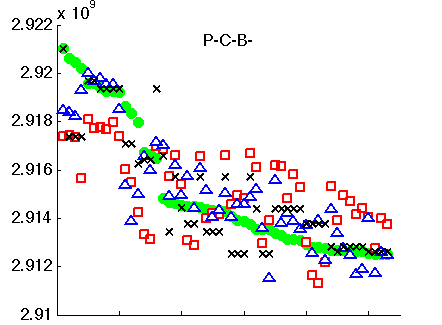
\includegraphics[scale = 0.34] {Figures/ooo_trainpredplot.png}
	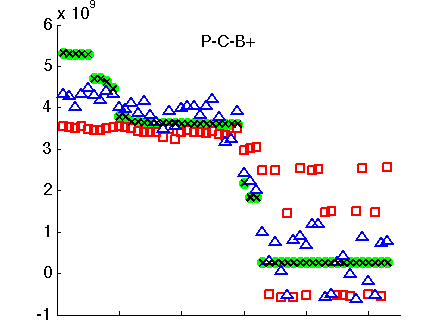
\includegraphics[scale = 0.34] {Figures/oop_trainpredplot.png}
	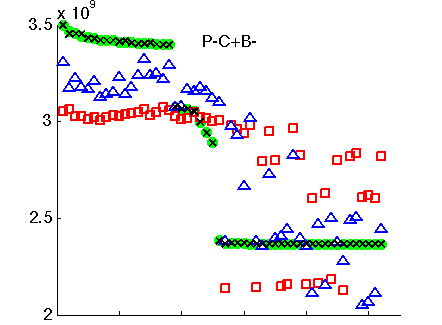
\includegraphics[scale = 0.34] {Figures/opo_trainpredplot.png}
	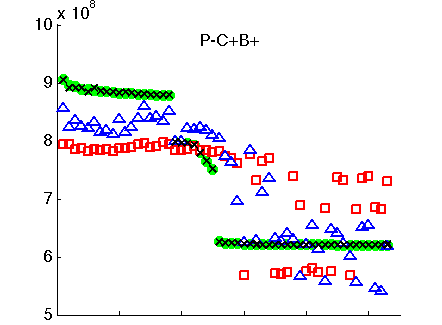
\includegraphics[scale = 0.34] {Figures/opp_trainpredplot.png}
	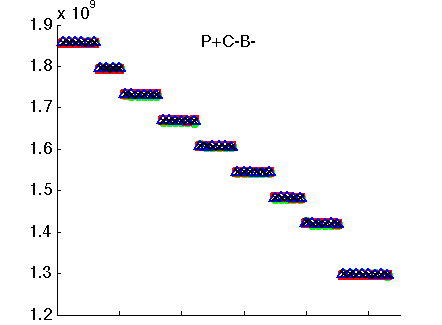
\includegraphics[scale = 0.34] {Figures/poo_trainpredplot.png}
	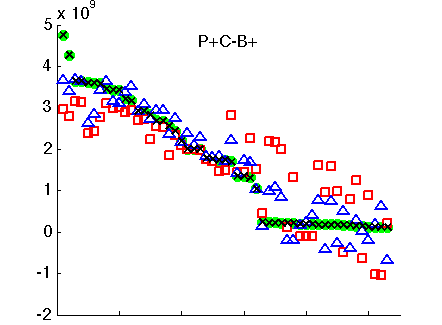
\includegraphics[scale = 0.34] {Figures/pop_trainpredplot.png}
	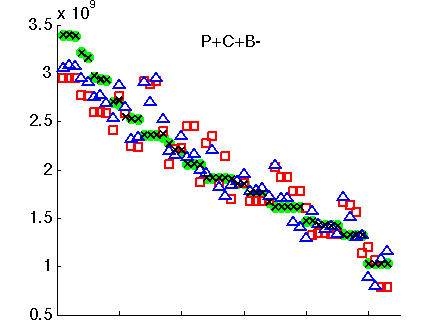
\includegraphics[scale = 0.34] {Figures/ppo_trainpredplot.png}
	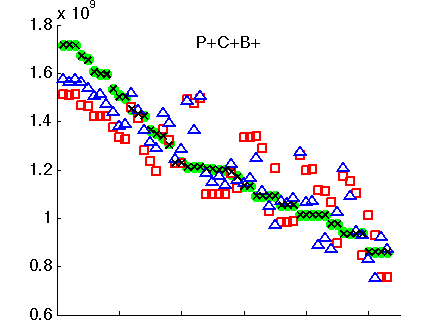
\includegraphics[scale = 0.34] {Figures/ppp_trainpredplot.png} \\
	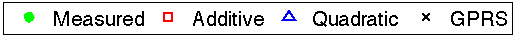
\includegraphics[scale = 0.5] {Figures/acc_comp_legend_horz.png}
	\caption{ \small Comparison of model accuracy for the eight microbenchmarks when predicting runtime in cycles. Each point represents a prediction for a machine configuration, and points are ordered along the x-axis based on decreasing measured run time. Y-axis plots predicted or measured runtime in cycles; note the differing ranges. In most cases, the nonlinear GPRS--based model is so accurate that it precisely captures all sample points.}
	\label{fig:acc}
\end{figure*}

%%\subsection{Partitioning Mechanism Efficacy}
%%It is worth noting that conflicts between different applications will always be destructive to performance and predictability.  The only danger to performance presented by hardware partitioning is the possibility of resource fragmentation, in which an application is allocated more of a resource than it can actually use.  However, a conservative allocation policy combined with fair sharing of excess resources can significantly mitigate this problem.

\subsubsection*{Evaluation of Model Accuracy}
In this section we examine the accuracy afforded by both the different linear regression models and the nonlinear GPRS--based regression model.  We choose a sample of 55 points from the space of 19200 possible allocations (or 0.3\%), and we train the models using this sample set.  The sample points were chosen using an Audze-Eglais DOE.

We evaluate the accuracy of the model relative to measured performance on a set of points disjoint from the sample set.  Due to the length of our simulations, we cannot exhaustively compare to all possible allocations and so limit our model error analysis to a testing set of 10 randomly selected points.  We perform this analysis for several performance metrics captured from simulation, including runtime in cycles, number of instructions committed, number of cache accesses, and number of off-chip memory accesses.

 Figure~\ref{fig:acc} plots the predictions versus measured data of a single performance metric for the sample set. While linear and nonlinear models perform equally well for some benchmarks, the nonlinear model is significantly more accurate at predicting others. The linear models struggle to capture the performance cliffs inherent to some benchmarks, especially those which move between being cache size-limited and bandwidth-limited.  In particular benchmarks which encounter a cliff and then saturate (such as the working set fitting in cache) are not faithfully modeled by the linear models.  The nonlinear model has no such difficulty.  It is also worth noting that the amount of error introduced in the linear additive and quadratic model causes them to predict negative values for some benchmarks.

\begin{table}
\small
\begin{tabular}{|l|c|c|c|}
\hline
Name & Additive & Quadratic & GPRS \\ \hline
 p--c--b-- & 0.06\% (0.04) & 0.04\% (0.04) &0.02\% (0.02) \\ \hline
 p--c--b+ &   234.07\% (287.44) & 139.21\% (167.10) &  0.23\% (0.40)   \\ \hline
 p--c+b-- &  12.67\% (5.30) &  8.26\% (5.30) &  0.02\% (0.02) \\ \hline
 p--c+b+ &  12.04\% (5.09) &  7.83\% (4.69) & 0.06\% (0.06)  \\ \hline
 p+c--b-- &  0.07\% (0.05) &  0.05\% (0.06)  &  0.05\% (0.03)  \\ \hline
 p+c--b+ &  271.05\% (377.53) & 164.23\% (226.23) & 0.51\% (1.08) \\ \hline
 p+c+b--&  13.08\% (6.91) & 8.79\% (7.32) & 0.06\% (0.07) \\ \hline
 p+c+b+&  12.07\% (4.86) &  8.05\% (5.49) & 0.08\% (0.06)  \\ \hline
   \end{tabular}
 \caption{Means (standard deviations) of percentage error in runtime cycles for each of the predictive models for each of the microbenchmarks.}
\label{table:acc-cycles}
\end{table}

\begin{table}
\small
\begin{tabular}{|l|c|c|c|}
\hline
Name & Additive & Quadratic & GPRS \\ \hline
 cluster &  4.27\% (3.66) & 6.90\% (5.67)  & 15.52\% (10.36)  \\ \hline
 gaussian&  1.83\% (0.72) & 4.16\% (2.49) & 2.33\% (3.19)  \\ \hline
 update&  4.98\% (3.04) & 7.94\% (7.12)  & 5.89\% (5.09)  \\ \hline
 pruning&  2.27\% (1.08) & 10.70\% (10.29)  & 3.07\% (2.91)  \\ \hline
 epsilon &  3.88\% (4.01) & 4.66\% (4.27)  & 2.69\% (1.09)  \\ \hline
   \end{tabular}
 \caption{Means (standard deviations) of percentage error in runtime cycles for each of the predictive models for each of the phases of the LVSRC application.}
\label{table:acc-cycles-lvsrc}
\end{table}

\begin{table}
\scriptsize
\begin{tabular}{|l|c|c|c|}
\hline
Name & Additive & Quadratic & GPRS \\ \hline
  p--c--b-- & 392.11\% (398.89) &  240.12\% (261.72) & 7.42\% (16.80)  \\ \hline
 p--c--b+ &  138133\% (290142)&  105682\% (248332) &  253.46\% (418.27)  \\ \hline
 p--c+b-- &   37225\% (65356) &  25797\% (47989) & 84.31\% (74.62)  \\ \hline
 p--c+b+ &   45276\% (82816) &  21819\% (30963) &  87.84\% (209.33)  \\ \hline
 p+c--b-- & 236.30\% (261.31) &  121.44\% (124.23) & 15.27\% (14.80)    \\ \hline
 p+c--b+ &   101696\% (169812)  &  73241\% (117426) & 25.42\% (31.95) \\ \hline
 p+c+b--&  16920\% (22871)&   12517\% (19362) & 7.47\% (8.25)  \\ \hline
 p+c+b+&   9480\% (11542) &  6647\% (9164) &  22.12\% (26.14)  \\ \hline
  \end{tabular}
 \caption{Means (standard deviations) of percentage error in offchip accesses for each of the predictive models for each of the microbenchmarks.}
\label{table:acc-offchip}
\end{table}

\begin{table}
\small
\begin{tabular}{|l|c|c|c|}
\hline
Name & Additive & Quadratic & GPRS \\ \hline
 p--c--b-- & 0.03\% (0.04) & 0.03\% (0.05) & 0.28\% (0.36) \\ \hline
 p--c--b+ & 241.91\% (262.05)  & 218.93\% (382.43) &  0.1\% (0.07) \\ \hline
 p--c+b-- & 8.49\% (5.49) & 6.17\% (6.50) & 0.41\% (1.13) \\ \hline
 p--c+b+ & 8.01\% (5.2)  & 5.79\% (6.11) & 0.07\% (0.06) \\ \hline
 p+c--b-- & 7.28\% (10.50)  & 0.05\% (0.04) & 0.27\%(0.19) \\ \hline
 p+c--b+ & 233.26\% (250.1) & 153.10\% (234.34) &  4.89\% (12.97)\\ \hline
 p+c+b-- & 20.23\% (24.18)  & 5.10\% (4.26) &  0.30\% (0.28) \\ \hline
 p+c+b+ & 13.30\% (10.23)  & 5.25\% (4.77)  & 0.05\% (0.03) \\ \hline
  \end{tabular}
 \caption{Means (standard deviations) of percentage error in cache transaction counts for each of the predictive models for each of the microbenchmarks.}
\label{table:acc-cache}
\end{table}

%\begin{table}
%\small
%\begin{tabular}{|l|c|c|c|}
%\hline
%Name & Cycles &Offchip Accesses &Cache Accesses \\ \hline
% p--c--b-- & 0.06\% (0.04) &  392.11\% (398.89) & 0.03\% (0.04) \\ \hline
% p--c--b+ &   234.07\% (287.44) & 138133\% (290142) & 241.91\% (262.05)  \\ \hline
% p--c+b-- &  12.67\% (5.30) & 37225\% (65356) & 8.49\% (5.49)  \\ \hline
% p--c+b+ &  12.04\% (5.09) &  45276\% (82816) & 8.01\% (5.2)  \\ \hline
% p+c--b-- &  0.07\% (0.05) &  236.30\% (261.31) & 7.28\% (10.50)  \\ \hline
% p+c--b+ &  271.05\% (377.53) & 101696\% (169812) & 233.26\% (250.1)  \\ \hline
% p+c+b--&  13.08\% (6.91) & 16920\% (22871) & 20.23\% (24.18)  \\ \hline
% p+c+b+&  12.07\% (4.86) &  9480\% (11542) & 13.30\% (10.23)  \\ \hline \hline
% cluster &  1 (1) & 1 (1)  & 1 (1)  \\ \hline
% gaussian&  1 (1) & 1 (1) & 1 (1)  \\ \hline
% update&  1 (1) & 1 (1)  & 1 (1)  \\ \hline
% pruning&  1 (1) & 1 (1)  & 1 (1)  \\ \hline
% epsilon &  1 (1) & 1 (1)  & 1 (1)  \\ \hline
% \end{tabular}
% \caption{Means (standard deviations) of percentage error for each of the performance measures for each of the benchmarks, as predicted by the linear response surface model.}
%\label{table:acc-lin}
%\end{table}
%
%\begin{table}
%\small
%\begin{tabular}{|l|c|c|c|}
%\hline
%Name & Cycles &Offchip Accesses &Cache Accesses \\ \hline
% p--c--b-- & 0.04\% (0.04) &  240.12\% (261.72) & 0.03\% (0.05) \\ \hline
% p--c--b+ &  139.21\% (167.10) &  105682\% (248332) & 218.93\% (382.43)  \\ \hline
% p--c+b-- &  8.26\% (5.30) &  25797\% (47989) & 6.17\% (6.50)  \\ \hline
% p--c+b+ &  7.83\% (4.69) &  21819\% (30963) & 5.79\% (6.11)  \\ \hline
% p+c--b-- &  0.05\% (0.06) &  121.44\% (124.23) & 0.05\% (0.04)  \\ \hline
% p+c--b+ &  164.23\% (226.23) &  73241\% (117426) & 153.10\% (234.34)  \\ \hline
% p+c+b--&  8.79\% (7.32) &   12517\% (19362) & 5.10\% (4.26)   \\ \hline
% p+c+b+&  8.05\% (5.49) &  6647\% (9164) & 5.25\% (4.77)  \\ \hline \hline
% cluster &  1 (1) & 1 (1) & 1 (1)  \\ \hline
% gaussian&  1 (1) & 1 (1) & 1 (1)  \\ \hline
% update&  1 (1) & 1 (1) &  1 (1)  \\ \hline
% pruning&  1 (1) & 1 (1) & 1 (1)  \\ \hline
% epsilon &  1 (1) & 1 (1) &  1 (1)  \\ \hline
% \end{tabular}
% \caption{Means (standard deviations) of percentage error for each of the performance measures for each of the benchmarks, as predicted by the quadratic response surface model.}
%\label{table:acc-quad}
%\end{table}
%
%\begin{table}
%\small
%\begin{tabular}{|l|c|c|c|}
%\hline
%Name & Cycles &Offchip Accesses &Cache Accesses \\ \hline
% p--c--b-- & 0.02\% (0.02) &   7.42\% (16.80) & 1 (1) \\ \hline
% p--c--b+ &  0.23\% (0.40) &  253.46\% (418.27) & 1 (1)  \\ \hline
% p--c+b-- &  0.02\% (0.02) &  84.31\% (74.62) & 1 (1)  \\ \hline
% p--c+b+ &  0.06\% (0.06) &  87.84\% (209.33) & 1 (1)  \\ \hline
% p+c--b-- &  0.05\% (0.03) &  15.27\% (14.80) & 1 (1)  \\ \hline
% p+c--b+ &  0.51\% (1.08) &  25.42\% (31.95) & 1 (1)  \\ \hline
% p+c+b--&  0.06\% (0.07) &  7.47\% (8.25)) & 1 (1)  \\ \hline
% p+c+b+&  0.08\% (0.06) &  22.12\% (26.14) & 1 (1)  \\ \hline \hline
% cluster &  1 (1) & 1 (1) &  1 (1)  \\ \hline
% gaussian&  1 (1) & 1 (1) & 1 (1)  \\ \hline
% update&  1 (1) & 1 (1)  & 1 (1)  \\ \hline
% pruning&  1 (1) & 1 (1) & 1 (1)  \\ \hline
% epsilon &  1 (1) & 1 (1) & 1 (1)  \\ \hline
% \end{tabular}
% \caption{Means (standard deviations) of percentage error for each of the performance measures for each of the benchmarks, as predicted by the GPRS model.}
%\label{table:acc-nonlin}
%\end{table}

Table~\ref{table:acc-cycles} reports the mean and standard deviation of percentage error of each of the models in predicting runtime cycles versus the measured performance of the test set. Table~\ref{table:acc-offchip} does the same for the off-chip accesses metric and Table~\ref{table:acc-cache} for the L2 cache transactions metric.  Points in the test set are not in the training set.

For some performance metrics the quadratic response surface models do a poor job of capturing the performance behavior of the points in the test set.  Linear additive model performance is even worse than the quadratic model, due mainly to the fact the the additive models lack interaction terms. However, the nonlinear models accurately capture the performance behavior of all metrics in most cases, with only a trouble areas, discussed below.

For all benchmarks, the number of instructions was relatively easy to predict, while the off-chip bandwidth and number of cache accesses were much more difficult.  Performance (cycles) prediction accuracy fell in between.  The benchmarks with the worst standard deviations had several extreme outliers that reduced the mean accuracy. Since the accuracy reported in the aforementioned tables is {\em percentage} error, it is subject to inflation when some absolute values being predicted are small relative to others in the set, which is the case particularly for off-chip bandwidth measurements.  Therefore, our judgement of model quality is dependent on how much we value accurate prediction of these small values.  For example, the GPRS--based model of microbenchmark \texttt{  p--c--b+}'s offchip accesses has a percentage error of 253.46\%, but this is caused by mispredictons of less than 5000 accesses (versus up to 2 million accesses incurred by the benchmark for certain resource allocations).

Our target machine runs Linux, which can add some non-determistic performance to the experiments.  A system with two-level scheduling would mostly likely see improved model accuracy.

While certain benchmarks are more challenging than others, there is no substantial difference in prediction accuracy between the synthetic benchmarks and real application. Table~\ref{table:acc-cycles-lvsrc} shows the accuracy of predictions of runtime (in cycles) per phase in terms of percentage error when measured against a test set.  The phases of the LVSRC application were actually more easily predicted than some of the microbenchmarks.  Due to the extreme length of the application (which was run to completion), the space of allocations we considered was limited to a maximum of two cores.  We reduced the size of the sample set correspondingly.  As a result, Table~\ref{table:acc-cycles-lvsrc} reflects models tuned on very small samples; with some adjustment of the genetic search parameters to prevent overfitting, all of the GPRS--based model percentage errors were reduced below 2\%.

%%For all of the applications, we can see that the models captured the performance of 90\% of the test points with less than []\% error.  This result leads us to believe that the model is an adequate enough representation of application performance to be useful in predicting performance for the remainder of the allocation options.

Clearly, the nonlinear models are extremely accurate and would make excellent input to our spatial resource allocation algorithm.  However, the GPRS--based models used here took between 0.5 and 6 hours each to build, so clearly they would have to be created offline and stored for use at runtime.  The linear models can be trained extremely rapidly, but are less accurate.  The true metric of whether or not a model is accurate ``enough'' depends on the quality of the decisions made based on it.
%We investigate decisions based on both linear and nonlinear model in Section~\ref{sec:decisions}.

\subsubsection*{Effect of Sample Size on Model Accuracy}
\label{sec:eval:acc-sample}

Figure ~\ref{fig:acc-sample} shows the impact that changing the sample set size has on model accuracy, using the example of execution time predictions for the microbenchmarks.  It is worth noting that while the accuracy of the quadratic and  nonlinear models improve rapidly with increasing sample size, the linear additive model sees no improvement on average.  This failure to improve when exposed to additional data indicates that it is the {\em form} of the model itself which is flawed (i.e. too simplistic).  Another important feature is that as sample size increases, the improvement seen by the other models slows, indicating a point of diminishing returns for increasing sample size.

This sample size analysis informs our decision about whether we can afford to use online or offline, linear or nonlinear models.  On the one hand, GPRS--based nonlinear models are much more accurate even when given smaller sample sizes.  However, they take a long time to train, and cannot be rapidly adapted to account for new data points.  On the other hand, linear models of sufficient complexity require more points to succeed, but can be rapidly trained and retrained.  A hybrid approach, in which genetic programming is used to construct the form of the response surface model offline, and then the model's coefficients are retuned based on performance data collected online, may a viable way to get the best of both worlds.

\begin{figure}
	\centering
	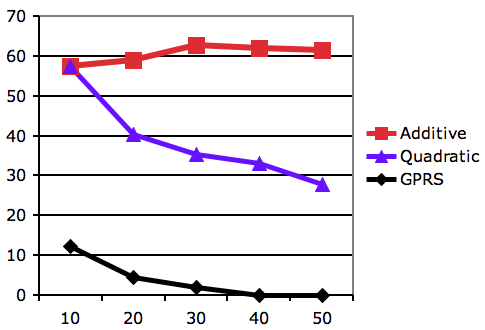
\includegraphics[scale = 0.5] {Figures/acc_sample.png}
	\caption{ \small Comparison of model accuracy for different models as training sample size is increased.  Y-axis is average percentage error in predictions of runtime averaged across all benchmarks. X-axis is increasing sample size.  Some models are more robust to reduced sample size than others.}
	\label{fig:acc-sample}
\end{figure}


\subsection{RTF Exploration and System Potential using an FPGA-based System Simulator}
~\cite{bird,tess_resource}



\subsubsection*{Experimental Setup}

We performed some of our own resource allocation experiments to
confirm that runtime hardware measurements can help improve OS
scheduling decisions.  Using an FPGA-based multiprocessor emulator RAMP Gold~\cite{rampgold09, rampgold10, fame10} and
a simple research operating system ROS~\cite{ros, tess,tess_resource}, we ran experiments with the Parsec
2.0 Benchmark Suite~\cite{parsec} and some handcrafted
microbenchmarks on a 64-core target machine. The OS uses page coloring
to allocate sections of the cache to an application, and the simulator
implements a simple form of bandwidth partitioning by limiting the
number of requests that can be sent to memory over a time
interval. Our system executes each of the applications several times,
each time varying the number of cores, and cache and bandwidth
allocations.  We collect application runtime performance data using
performance measurement hardware to create models of the performance
for that application given a particular resource allocation.  We
created a quadratic model and linear model with multivariate
regression techniques, a GPRS model, and a KCCA model using 20\% of the possible allocations.  Using
these models, our scheduler decides how best to run a mix of two
applications by trying to optimize a given objective function.  For
these results, we chose a simple proxy for total energy consumed, the
total number of cycles run (the sum of the cycles on each core) +
10$\times$ the total number of off-chip accesses, as our example
objective function.

Our experimental platform for this case study consists of five Xilinx
XUP FPGA boards. Each board is programmed to simulate one instance of
our target architecture.  Table~\ref{table:target} lists the target
machine parameters. We run six applications from the PARSEC benchmark
suite \cite{parsec}, as well as two synthetic microbenchmarks.
Table~\ref{table:benchmarks} summarizes the benchmarks. The
performance models are built based on applications running alone on a
partition of the machine but are tested against data collected from
multiprogrammed scheduling scenarios.  We simulated all possible
allocations for each benchmark running alone, and then all possible
schedules of allocations for 3 pairs of benchmarks running
simultaneously, for a combined total of 68.5 trillion target
core-cycles.  (A core-cycle is 1 clock cycle of execution on 1 core;
simulating a 64-core CMP for 1,000,000 cycles would be 64,000,000
core-cycles.)

 The Research Operating System (ROS) is a prototype operating system
 build to investigate OS design principles in the manycore era
 \cite{tess, tess_resource, tess_dac}.  We ported ROS to boot on Midas FAME, and
 modified its functionality to support our scheduling framework
 (including paging management and threading libraries).


Our spatial scheduling framework is implemented within a prototype
research operating system (ROS) that runs on the target machine
simulated by Midas FAME~\cite{ros}.


\begin{table*}[ct]
 \begin{center}
\footnotesize
\begin{tabular}{|c|l|}
\hline
 Attribute  & Setting \\ \hline \hline
 CPUs & 64 single-issue in-order cores @ \wunits{1}{GHz} \\ \hline
 L1 Instruction Cache & Private, \wunits{32}{KB}, 4-way set-associative, 128-byte lines \\ \hline
 L1 Data Cache & Private, \wunits{32}{KB}, 4-way set-associative, 128-byte lines \\ \hline
 L2 Unified Cache & Shared, \wunits{8}{MB}, 16-way set-associative, 128-byte lines, inclusive, 4 banks, \wunits{10}{ns} latency \\ \hline
 Off-Chip DRAM & \wunits{2}{GB}, 4$\times$\wunits{3.2}{GB/sec} channels,
 \wunits{70}{ns} latency \\ \hline
 \end{tabular}
\caption{Target machine parameters simulated by RAMP Gold.}
\label{table:target}
 \end{center}
\end{table*}

\begin{table*}[ct]
 \begin{center}
\footnotesize
\begin{tabular}{|l|l|l|r|l|}
\hline
 Name  & Type & Parallelism & Working Set & Bandwidth Demand\\ \hline \hline
Blackscholes & financial PDE solver & coarse data parallel & \wunits{2.0}{MB} & minimal \\ \hline
Bodytrack & vision & medium data parallel & \wunits{8.0}{MB} & grows with cores\\ \hline
Fluidanimate & animation & fine data parallel & \wunits{64.0}{MB} & grows with cores\\ \hline
Streamcluster & data mining & medium data parallel & \wunits{16.0}{MB} & high \\ \hline
Swaptions & financial simulation & coarse data parallel & \wunits{0.5}{MB} & grows with cores \\ \hline
x264 & media encoder & pipeline & \wunits{16.0}{MB} & grows with cores \\ \hline \hline
Tiny & synthetic &  one thread does all work & \wunits{1}{KB} & minimal \\ \hline
Greedy & synthetic & data parallel & \wunits{16.0}{MB} & high \\ \hline
\end{tabular}
\caption{Benchmark description. PARSEC benchmarks use \texttt{ simlarge} input set sizes, except for x264 and fluidanimate, which use \texttt{ simmedium} due to limited physical memory capacity.  PARSEC characterizations are from \cite{parsec}.}
\label{table:benchmarks}
 \end{center}
\end{table*}


\paragraph*{Partitioning Mechanisms}
Our allocation framework includes the following resources: the cores
and their private caches, the shared last-level cache, and shared
memory bandwidth.  For each resource, we provide a mechanism to
prevent applications from exceeding their allocated share. The OS
assigns cores and their associated private resources to a specific
application. For the shared last-level cache, we modify the OS
page-coloring algorithm so that applications are never given a page
from a different application's color allocation.

To partition off-chip memory bandwidth, we use Globally-Synchronized
Frames (GSF)\cite{gsf}. GSF provides strict Quality-of-Service
guarantees for minimum bandwidth and the maximum delay of a
point-to-point network---in our case the memory network---by
controlling the number of packets that each core can inject per frame.
We use a modified version of the original GSF design, which tracks
allocations per application instead of per core, does not reclaim
frames early, and does not allow applications use the excess
bandwidth.  These changes make GSF more suited to our study since we
want to strictly bound the maximum bandwidth per application.
Implementing GSF required some modifications to the target machine's
memory controller in RAMP Gold to synchronize the frames and track
application packet injections.  Due to the functional/timing split in
RAMP Gold, this modification was no more difficult than modifying a
software simulator would have been.

\paragraph{RTF Construction}

 We use a design of experiments (DoE) technique known as the Audze-Eglais
Uniform Latin Hypercube design of experiments \cite{bates-aes03} to
select the points included in the sample set.  Audze-Eglais selects
sample points which are as evenly distributed as possible through the
space of possible allocations.

To explore the relationship between model accuracy and model type
for our problem space, we evaluate linear additive models, quadratic
response surface models, and non-linear models based on Kernel Canonical Correlation Analysis (KCCA) \cite{kcca} and GPRS.

The simplest models we consider are linear additive models, which
contain one term for each variable (i.e. an allocation type) and one
coefficient associated which each term.  Linear additive models
ignore any possible interaction between the variables, an invalid
assumption in our scheduling scenario.  For this reason, we also
include more complex multivariate regression models, commonly termed
`response surface models', which include terms for variable
interaction and polynomial terms of degree 2 or more.  We also employ
Kernel Canonical Correlation Analysis (KCCA) \cite{kcca} as a
representative example of even more complex nonlinear modeling
techniques. KCCA automatically detects correlations among the
variables and outputs included in the model, and uses this analysis
to make predictions.


\paragraph{Resource Allocation Decisions}

The scheduler uses the models for each application to decide how best
to divide resources up between a mix of applications all running
concurrently.  Our initial prototype scheduler optimizes the
reassignment of spatial resource allocations without regard to the
current allocations and the resulting reallocation overhead.  Even
this simplified problem is combinatorial (and in fact is
NP-hard). The algorithm works by maximizing an objective function,
which serves to convert model outputs into a measure of overall
decision fitness.  The form of the objective function influences the
type of algorithm we can use to maximize fitness. We use Matlab's
\cite{matlab} implementation of the medium-scale active-set
algorithm, which is a sequential quadratic programming based solver
and so depends on the convexity of the function to guarantee
optimality.

Only some of our objective functions are convex, and the optimization
algorithm may choose local minima for ones which are not.  As a
result, even with perfect models the scheduler could pick non-optimal
solutions.  For this reason, it is important to experiment with
different model types, sample sizes, objective functions, and
maximization algorithms to find the right balance between system
complexity and accuracy of scheduling decisions.




\subsubsection*{Case Study Results}

\begin{figure*}[htb]
%        \center{\includegraphics[width=1.1\textwidth]
	\noindent\makebox[\textwidth]{%
        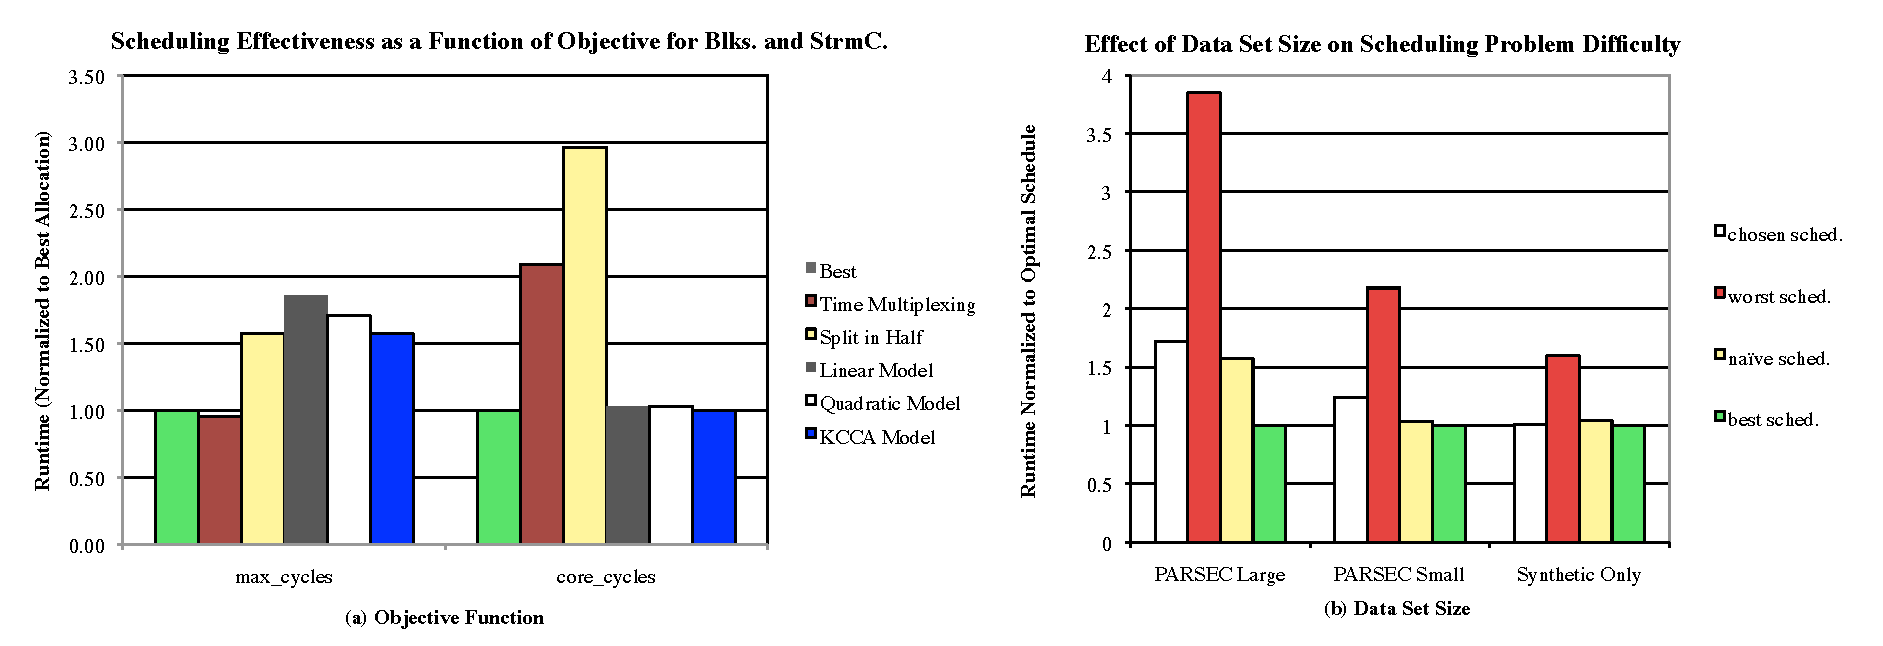
\includegraphics[width=1.0\textwidth]
        {Figures/case_study_outcome.pdf}}
        \caption{\label{fig:case_study_outcome}  (a) The performance
          of various scheduling methodologies and objective functions
          for one scheduling problem, normalized to the globally
          optimal schedule's performance.  The scheduler tries to
          minimize each objective function.  (b) The effect of
          benchmark size on the difficulty of the scheduling problem.
          The average chosen schedule performance, global worst case
          and naive scheduling case are normalized to the globally
          optimal schedule's performance for each dataset. The
          scheduling decision is Blackscholes vs. Streamcluster, the
          objective function is to minimize runtime.
 }
\end{figure*}

We found that predictive modeling has potential to successfully manage
some applications, depending on the scheduler's objective function.
For example, if the objective is to minimize energy, the approach
works quite well.  However, if the objective is to minimize the time
it takes to complete both applications, the naive baselines, such as
splitting the machine in half or time-multiplexing, often performed as
well or significantly better than model-based
allocation. Figure~\ref{fig:case_study_outcome}(a) presents an example
of these results. More importantly, our conclusions about the value of
model-based scheduling would have been different had we \emph{not}
simulated the entire execution of benchmarks, with large input sets,
for all possible allocations.

\begin{figure}[tb]
  \begin{center}
    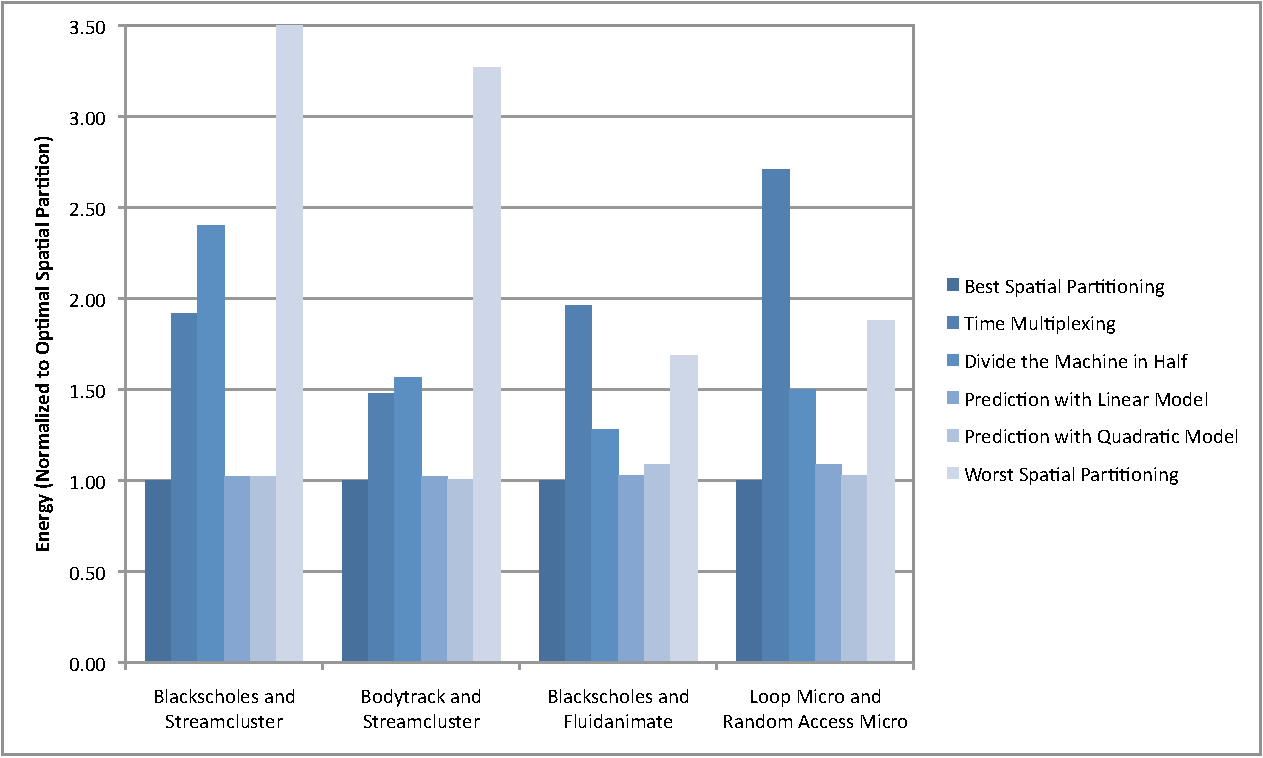
\includegraphics[width=\linewidth]{Figures/scheduling_results_energy.pdf}
  \end{center}
  \caption{Comparison of the effectiveness of different scheduling
    techniques normalized to our quadratic model-based approach.  The
    metric (sum of cycles on all cores + 10$\times$ sum of off-chip
    accesses) is a proxy for energy, so lower numbers are better.}
  \label{fig:scheduling_results}
\end{figure}




Figure~\ref{fig:scheduling_results} shows the results of our
scheduler's decisions based on the runtime performance data as
compared with several alternatives: the optimal allocation, naively
giving each application half of the machine, or time-multiplexing each
application across the entire machine.  The time-multiplexing scheme
first runs the first application to completion and then runs the
second application to completion.  More fined-grained
time-multiplexing could lead to longer runtimes due to cache
interference effects and other context swap overheads.

We do no show results for the GPRS and KCCA as we found that they were extremely non-convex and as a result often produced very poor results when paired with our optimizer. The simple linear and quadratic models perform much better with only a small set of sample points and have significantly lower overhead.

The results
show that using runtime data to perform more intelligent scheduling
can lead to a significant savings in time and energy.  Our approach
beats naively dividing the machine by 65\% and time multiplexing by
100\% on average. Furthermore, it is within a few percent of optimal
every time.  The worst-case results show that the penalty for poor
decision making can be quite large, with an energy cost 3.25$\times$
greater than our allocation on average.

As the number of cores and other shared resources grows on chip, this
will increase the number of possible allocations, thereby widening the
performance gap between good and bad schedules.  Additionally, we
expect that much more code will be tuned for parallel execution, and
exhibit a greater variety of behaviors.  As a result, there will more
likely be disjoint resource requirements among applications available
to co-schedule.  We believe hardware measurement-based scheduling will
thus prove even more effective.


\subsection{\pacora Feasibility in a Real System}
Our static framework was designed to test the effectiveness of \pacora's model-based convex optimization for allocating resources.  We used it to experiment with the accuracy of different types of models and test the quality of the resource allocation decisions. Data is collected online by running application benchmarks on a recent x86 processor running Linux-2.6.36.  The measured data is processed using Python and then fed to MATLAB~\cite{matlab} to build the RTFs.  MATLAB uses the RTFs to make resource allocation decisions.  We compare performance of the chosen resource allocations with the actual measured performance of all possible resource allocations to test quality of the resource allocation decisions. We use CVX~\cite{cvx} in MATLAB to perform the convex optimization for building RTFs and making resource allocation decisions.  We chose this static approach because it let us test many applications, 44 in total, and many resource allocations rapidly.

\subsubsection{Platform}

To collect data, we use a prototype version of Intel's Sandy Bridge x86 processor that is similar to the
commercially available client chip, but with additional hardware
support for way-based LLC partitioning.
The Sandy Bridge client chip has 4 quad-issue out-of-order
superscalar cores, each of which supports 2 hyperthreads using
simultaneous multithreading~\cite{IntelRefManual:2011}.
%Each core has private \wunits{32}{KB} instruction and data caches, as well as a
%\wunits{256}{KB} private non-inclusive L2 cache.
The LLC is a 12-way
set-associative \wunits{6}{MB} inclusive L3 cache, shared among all
cores using a ring-based interconnect.
%All three cache levels are write-back.
The cache partitioning mechanism is way-based and works by modifying the
cache-replacement algorithm.  To allocate cache ways, we assign a subset of
the 12 ways to a set of hyperthreads, thereby allowing only those hyperthreads to replace data in those ways.

%Way allocations can be completely private,
%completely shared, or overlapping.  Although all cores can hit on data stored in
%any way, a core can only replace data in its assigned
%ways.   Data is not flushed when the way allocation changes.

We use a customized BIOS that enables the cache partitioning
mechanism, and run unmodified Linux-2.6.36 for all of our experiments.
To allocate cores, we use the Linux \texttt{taskset} command to pin applications to
sets of hyperthreads. The standard Linux scheduler performs the scheduling for applications within these containers of hyperthreads. For our experiments we consider each hyperthread to be an independent core. To minimize inter-application interference, we first assign both hyperthreads available in one core before moving on to the next core. For example, a 4-core allocation from \pacora represents 4 hyperthreads on 2 cores on the machine.

\subsubsection{Performance and Energy Measurement}

To measure application performance, we use the \texttt{libpfm}
library~\cite{Eranian:OLS06,Perfmon2}, built on top of the
\texttt{perf\_events} infrastructure in Linux, to
access available performance counters~\cite{Intel:Manual2012}.

To measure on-chip energy, we use the energy counters available on
Sandy Bridge to measure the consumption of  the entire socket and also
the total combined energy of cores, their private caches, and the
LLC. We access these counters using the Running Average Power Limit
(RAPL) interfaces~\cite{Intel:Manual2012}.  %The counters measure power
%at a $1/2^{16}$ second granularity.

%In addition, we use a FitPC external multimeter to measure at the wall socket the power
%consumed by the entire system, at a
%\wunits{1}{second} granularity.
%We correlate the wall power data with the data collected from the hardware energy counters
%using time stamps.  We observed less than one second of delay in these
%measurements consistently across all experiments.  Together, these
%mechanisms allow us to collect accurate energy readings over the
%entire course of an application's execution.

\subsubsection{Description of Workloads}

Our workload contains a range of applications from three different
popular benchmark suites: SPEC CPU 2006~\cite{SPEC2006},
DaCapo~\cite{dacapo}, and PARSEC~\cite{parsec}. We selected this set of applications to represent a wide variety of possible resource behaviors in order to properly stress \pacora's RTFs. We include some additional applications to broaden the
scope of the study, and some microbenchmarks to exercise certain
system features.

The \textbf{SPEC CPU2006} benchmark suite~\cite{SPEC2006} is a
CPU-intensive, single-threaded benchmark suite, designed to stress a
system's processor, memory subsystem, and compiler.  Using the
similarity analysis performed by Phansalkar \emph{et
al.}~\cite{Phansalkar:ISCA2007}, we subset the suite, selecting 4
integer benchmarks (\texttt{ astar}, \texttt{ libquantum}, \texttt{ mcf}, \texttt{ omnetpp}) and 4
floating-point benchmarks (cactusADM, calculix, lbm, povray).  Based
on the characterization study by Jaleel~\cite{Jaleel:TR2007}, we also
pick 4 extra floating-point benchmarks that stress the LLC: \texttt{ GemsFDTD},
\texttt{ leslie3d}, \texttt{ soplex} and \texttt{ sphinx3}.  When multiple input sets are
available, we pick the single \textit{ref} input indicated by~\cite{Phansalkar:ISCA2007}.

We include the \textbf{DaCapo} Java benchmark suite as a
representative of managed-language workloads. We use the latest 2009 release, which consists of a set of open-source, real-world
applications with non-trivial memory loads, and includes both client and
server-side applications.

The \textbf{PARSEC} benchmark suite is intended to be representative
of parallel real-world applications~\cite{parsec}. PARSEC
programs use various parallelization approaches, including data- and
task-parallelization. We use native input sets and the \texttt{ pthreads} version for all benchmarks, with the exception of
\texttt{freqmine}, which is only available in OpenMP.

We add four \textbf{additional parallel applications} to help ensure
we cover the space of interest: \texttt{ Browser\_animation} is a
multithreaded kernel representing a browser layout animation; \texttt{
  G500\_csr} code is a breadth-first search algorithm; \texttt{ Paradecoder} is a parallel
speech-recognition application that takes audio waveforms of human
speech and infers the most likely word sequence intended by the
speaker; \texttt{ Stencilprobe} simulates heat transfer in a fluid
using a parallel stencil kernel over a regular
grid~\cite{Kamil:Stencilprobe}.

We also add two \textbf{microbenchmarks} that stress the memory
system and cause increased interference between applications: \texttt{ stream\_uncached} is a memory and on-chip bandwidth hog
that continuously brings data from memory without caching it, while
\texttt{ ccbench} explores arrays of different sizes to determine the
structure of the cache hierarchy.

Using a performance characterization of the applications, we select a subset of the benchmarks that are representative of different possible responses to resource allocations in order to reduce our study to a feasible size.  Similar to \cite{Phansalkar:ISCA2007}, we use machine learning to select representative benchmarks.  We use a
hierarchical clustering algorithm~\cite{Phansalkar:ISCA2007} provided by the Python library \texttt{scipy-cluster} with the \textit{single-linkage} method.  The feature vector contains parameters to represent core scaling, cache scaling, prefetcher sensitivity and bandwidth sensitivity.  The clustering algorithm uses Euclidean distance between vectors to determine clusters.

The clustering results in 6 clusters representing the following (applications at the cluster center are listed in parenthesis):
 \begin{itemize}\itemsep0pt \parskip0pt \parsep5pt
\item no scalability, high cache utility, (\texttt{ 429.mcf})
\item no scalability, low cache utility, (\texttt{ 459.gems\-FDTD})
\item high scalability, low cache utility, (\texttt{ ferret})
\item limited scalability, high cache utility, (\texttt{ fop})
\item limited scalability, low cache utility, (\texttt{ dedup})
\item limited scalability, low bandwidth sensitivity, (\texttt{ batik})
\end{itemize}

%First, we create a feature vector for each application using the values in the previous subsection:
%1) execution time as we increase the number of threads; 2) execution time as we increase the LLC size; 3) prefetcher sensitivity; and 4) bandwidth sensitivity. All metrics are normalized to the interval $[0,1]$. In total we use vectors with 19 features ($7+10+1+1$).

%The clustering algorithm finds the smallest Euclidean distance of a pair of feature vectors and forms a cluster containing that pair. It continues selecting the next smallest distance between a pair and forms another cluster. Linkage criteria can be used to adjust cluster formation. The single-linkage we selected uses the minimum distance between a pair of objects in different clusters to determine the distance between them.

\subsubsection{RTF Experiments}
\begin{figure*}[!t]
	\begin{center}	
		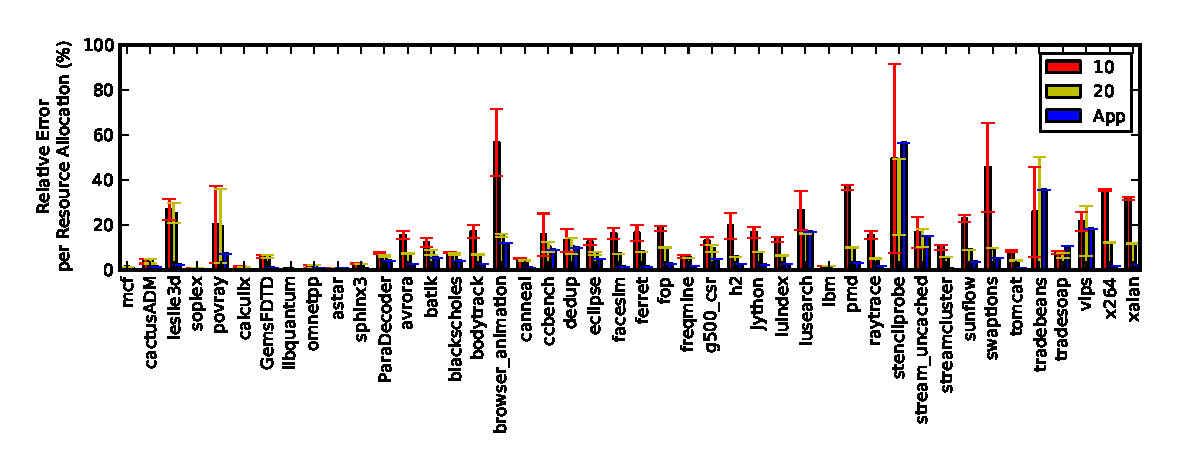
\includegraphics[bb=0 0 576 216,width=\textwidth]{Figures/model_accuracy.pdf}
		\caption{1-norm of relative error from RTF predicted response time compared to actual response time.  The actual response time is the median over 3 trials. 10 and 20 represent RTFs built with 10 and 20 training points respectively.  App represents the variability (average standard deviation) in performance of the application between the 3 trials.}
		\label{model_accuracy}
	\end{center}
\end{figure*}
To test the effectiveness of our RTFs in capturing real application behavior, we measure each of our 44 benchmarks running alone on the machine for all possible resource allocations of cache ways and cores.  Cores can be allocated from 1--8 and cache ways from 1--12 resulting in 96 possible allocations for each application.   We use a genetic algorithm design of experiments~\cite{bates-aes03} to select 10 and 20 of the collected allocations to build the RTFs.  We also experimented with building RTFs with more data points but found that they provided little improvement over 20~\cite{pacora_tr}.  We then use the model to predict the performance of every resource allocation and compare it with the actual measured performance (median value of 3 trials) of that resource allocation.  We built 3 different models from 3 trials and tested each of them against median measured value.

Figure~\ref{model_accuracy} shows the 1-norm of the relative error of the predicted response times per resource allocation for an RTF built with 10 training points and one built with 20.  The average error per point is 16\% for an RTF built with 10 training points and 9\% for an RTF built with 20 training points.  We also calculated the percentage variability (average standard deviation) for each resource allocation in the application between the 3 trials (shown as ``App'' in Figure~\ref{model_accuracy}).  The average variability is 9\%, so we can see that \pacora's RTFs are not much more inaccurate than the natural variation in response time in the application.  It is not for possible an RTF to be more accurate than the application variability, and we can also see that applications with higher variability result in RTFs with larger relative errors, (\emph{e.g.,} \texttt{stencilprobe}, \texttt{ tradebeans}).  Section~\ref{discuss} discusses application variability in more detail.

\subsubsection{Resource Allocation Experiments}
\begin{figure}[!t]
	\begin{center}	
		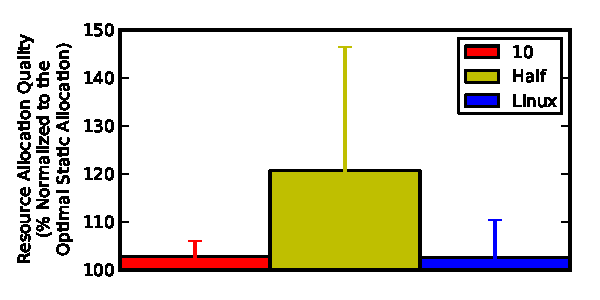
\includegraphics[bb=0 0 288 144,width=\columnwidth]{Figures/decision_quality.pdf}
		\caption{Resource allocation decisions for each pair of the cluster representative applications compared equally dividing the machine and a shared resources Linux baseline. Quality is measured is allocation performance divided by performance of the best possible allocation.}
		\label{decision_quality}
	\end{center}
\end{figure}


Using the RTFs built for the applications, we let \pacora make static resource allocations for all possible pairs of the cluster representative applications.  We then run an exhaustive study of all possible resource allocations for each pair on our Sandy Bridge-Linux platform, measure the performance, and compare it with the best performing, \emph{i.e.,} optimal, resource allocation.  We also compare this result to equally dividing the resources between the two applications and to sharing all of the resources using the standard Linux scheduler.

%how \pacora's decisions compared with the optimal allocation, equally dividing the machine, and the Linux baseline for each pair of the cluster representative applications.
Figure~\ref{decision_quality} shows these results for our 10 point RTFs. As we might expect, simple naive heuristics do not perform well, and dividing the machine in half is around 20\% slower than either \pacora or standard Linux.
 \pacora's resource allocations are 2\% from the optimal static allocation on average.  Using shared resources with the standard Linux scheduler performs similarly but with a higher standard deviation.  The shared resources comparison is interesting: while most of the time sharing resources can result in higher utilization, as the applications can dynamically take advantage of available resources, in some cases the interference between applications was so harmful to performance that on average optimal static partitioning performs slightly better.  As a result \pacora is able to provide performance comparable to Linux scheduling on shared resources with more predictable performance on average (lower worst cases).  Additionally, as the shown in the next Section, \pacora's resource allocation decisions do not need to be static, but can be made dynamically to adjust to the changing needs of the applications.
%These results indicate the \pacora is able to get a near optimal resource allocation and match the performance of the traditional Linux scheduler with more predictability.

\subsubsection{Effect of Model Accuracy on Decision Quality}

\begin{figure}[!t]
	\begin{center}	
%		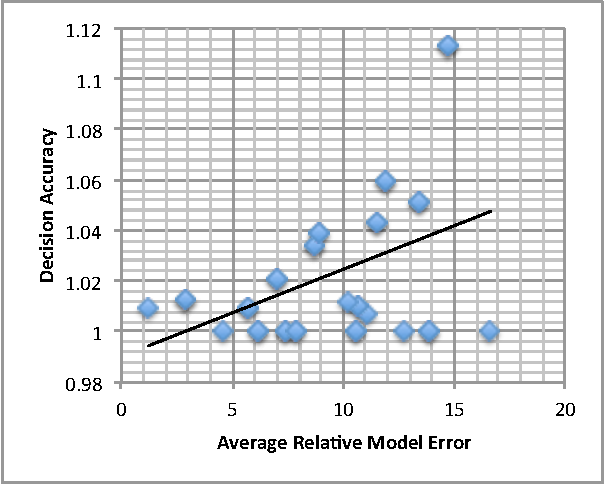
\includegraphics[width=0.9\textwidth]{cluster_decision_accuracy.pdf}
		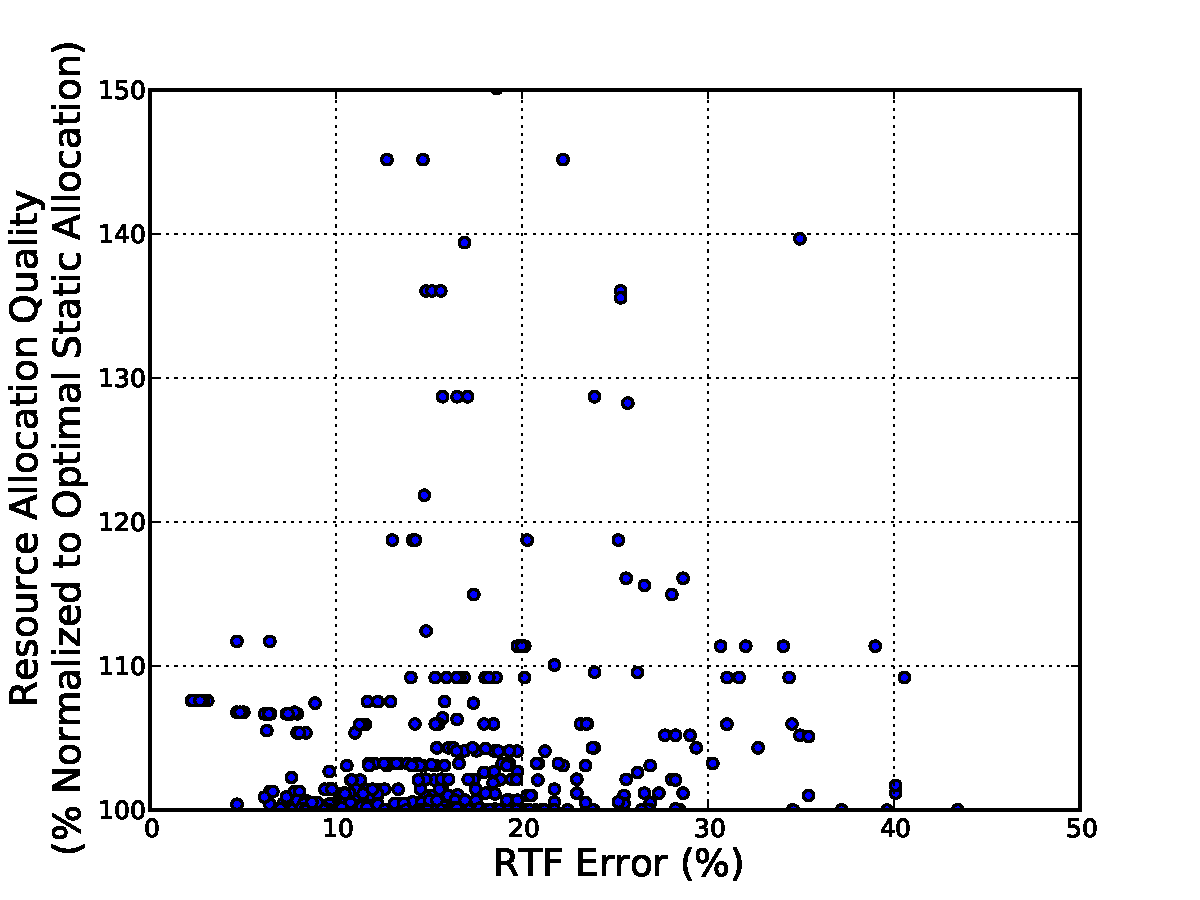
\includegraphics[bb=0 0 576 432,width=\columnwidth]{Figures/accuracy_quality.pdf}
		\caption{Effect of Model Accuracy on Decision Quality. The x axis represents the combined relative error of all RTFs used in the decision.}
		\label{accuracy_quality}
	\end{center}
\end{figure}


There are two main sources of challenges for \pacora's design: performance non-convexity and performance variability. 
The main concern with performance non-convexity and variability is their effects on the accuracy of the response time functions.  However, an important result we have found while evaluating \pacora is that model accuracy has less impact on the quality of resource allocation decisions than we anticipated.  When experimenting with possible models for the RTFs, we found that while some models were always a little too inaccurate and did degrade the performance of the resource allocation decisions, once a model crossed a certain threshold of accuracy then better models provided insignificant improvement in resource allocation decisions. Figure~\ref{accuracy_quality} shows the effect of model accuracy on the quality of the resource allocation decisions made using the RTF model in Equation~\ref{rtf_eq}.  Although there is a slight correlation between model accuracy and decision quality, many decisions with inaccurate models still result in near optimal allocations.  This effect enables \pacora's model-based design to be feasible in a noisy system with real applications.

%------------------------------------------------------------------------------------------------------------------------------------------------------------------------
\chapter{RTF Exploration and Feasibility Study}\label{init_eval}
%------------------------------------------------------------------------------------------------------------------------------------------------------------------------

We perform 2 studies to test the potential of PACORA for resource allocation.

\subsection{RTF Exploration and System Potential using an FPGA-based System Simulator}
~\cite{bird,tess_resource}



\subsubsection*{Experimental Setup}

We performed some of our own resource allocation experiments to
confirm that runtime hardware measurements can help improve OS
scheduling decisions.  Using an FPGA-based multiprocessor emulator RAMP Gold~\cite{rampgold09, rampgold10, fame10} and
a simple research operating system ROS~\cite{ros, tess,tess_resource}, we ran experiments with the Parsec
2.0 Benchmark Suite~\cite{parsec} and some handcrafted
microbenchmarks on a 64-core target machine. The OS uses page coloring
to allocate sections of the cache to an application, and the simulator
implements a simple form of bandwidth partitioning by limiting the
number of requests that can be sent to memory over a time
interval. Our system executes each of the applications several times,
each time varying the number of cores, and cache and bandwidth
allocations.  We collect application runtime performance data using
performance measurement hardware to create models of the performance
for that application given a particular resource allocation.  We
created a quadratic model and linear model with multivariate
regression techniques, a GPRS model, and a KCCA model using 20\% of the possible allocations.  Using
these models, our scheduler decides how best to run a mix of two
applications by trying to optimize a given objective function.  For
these results, we chose a simple proxy for total energy consumed, the
total number of cycles run (the sum of the cycles on each core) +
10$\times$ the total number of off-chip accesses, as our example
objective function.

Our experimental platform for this case study consists of five Xilinx
XUP FPGA boards. Each board is programmed to simulate one instance of
our target architecture.  Table~\ref{table:target} lists the target
machine parameters. We run six applications from the PARSEC benchmark
suite \cite{parsec}, as well as two synthetic microbenchmarks.
Table~\ref{table:benchmarks} summarizes the benchmarks. The
performance models are built based on applications running alone on a
partition of the machine but are tested against data collected from
multiprogrammed scheduling scenarios.  We simulated all possible
allocations for each benchmark running alone, and then all possible
schedules of allocations for 3 pairs of benchmarks running
simultaneously, for a combined total of 68.5 trillion target
core-cycles.  (A core-cycle is 1 clock cycle of execution on 1 core;
simulating a 64-core CMP for 1,000,000 cycles would be 64,000,000
core-cycles.)

 The Research Operating System (ROS) is a prototype operating system
 build to investigate OS design principles in the manycore era
 \cite{tess, tess_resource, tess_dac}.  We ported ROS to boot on Midas FAME, and
 modified its functionality to support our scheduling framework
 (including paging management and threading libraries).


Our spatial scheduling framework is implemented within a prototype
research operating system (ROS) that runs on the target machine
simulated by Midas FAME~\cite{ros}.


\begin{table*}[ct]
 \begin{center}
\footnotesize
\begin{tabular}{|c|l|}
\hline
 Attribute  & Setting \\ \hline \hline
 CPUs & 64 single-issue in-order cores @ \wunits{1}{GHz} \\ \hline
 L1 Instruction Cache & Private, \wunits{32}{KB}, 4-way set-associative, 128-byte lines \\ \hline
 L1 Data Cache & Private, \wunits{32}{KB}, 4-way set-associative, 128-byte lines \\ \hline
 L2 Unified Cache & Shared, \wunits{8}{MB}, 16-way set-associative, 128-byte lines, inclusive, 4 banks, \wunits{10}{ns} latency \\ \hline
 Off-Chip DRAM & \wunits{2}{GB}, 4$\times$\wunits{3.2}{GB/sec} channels,
 \wunits{70}{ns} latency \\ \hline
 \end{tabular}
\caption{Target machine parameters simulated by RAMP Gold.}
\label{table:target}
 \end{center}
\end{table*}

\begin{table*}[ct]
 \begin{center}
\footnotesize
\begin{tabular}{|l|l|l|r|l|}
\hline
 Name  & Type & Parallelism & Working Set & Bandwidth Demand\\ \hline \hline
Blackscholes & financial PDE solver & coarse data parallel & \wunits{2.0}{MB} & minimal \\ \hline
Bodytrack & vision & medium data parallel & \wunits{8.0}{MB} & grows with cores\\ \hline
Fluidanimate & animation & fine data parallel & \wunits{64.0}{MB} & grows with cores\\ \hline
Streamcluster & data mining & medium data parallel & \wunits{16.0}{MB} & high \\ \hline
Swaptions & financial simulation & coarse data parallel & \wunits{0.5}{MB} & grows with cores \\ \hline
x264 & media encoder & pipeline & \wunits{16.0}{MB} & grows with cores \\ \hline \hline
Tiny & synthetic &  one thread does all work & \wunits{1}{KB} & minimal \\ \hline
Greedy & synthetic & data parallel & \wunits{16.0}{MB} & high \\ \hline
\end{tabular}
\caption{Benchmark description. PARSEC benchmarks use \texttt{ simlarge} input set sizes, except for x264 and fluidanimate, which use \texttt{ simmedium} due to limited physical memory capacity.  PARSEC characterizations are from \cite{parsec}.}
\label{table:benchmarks}
 \end{center}
\end{table*}


\paragraph*{Partitioning Mechanisms}
Our allocation framework includes the following resources: the cores
and their private caches, the shared last-level cache, and shared
memory bandwidth.  For each resource, we provide a mechanism to
prevent applications from exceeding their allocated share. The OS
assigns cores and their associated private resources to a specific
application. For the shared last-level cache, we modify the OS
page-coloring algorithm so that applications are never given a page
from a different application's color allocation.

To partition off-chip memory bandwidth, we use Globally-Synchronized
Frames (GSF)\cite{gsf}. GSF provides strict Quality-of-Service
guarantees for minimum bandwidth and the maximum delay of a
point-to-point network---in our case the memory network---by
controlling the number of packets that each core can inject per frame.
We use a modified version of the original GSF design, which tracks
allocations per application instead of per core, does not reclaim
frames early, and does not allow applications use the excess
bandwidth.  These changes make GSF more suited to our study since we
want to strictly bound the maximum bandwidth per application.
Implementing GSF required some modifications to the target machine's
memory controller in RAMP Gold to synchronize the frames and track
application packet injections.  Due to the functional/timing split in
RAMP Gold, this modification was no more difficult than modifying a
software simulator would have been.

\paragraph{RTF Construction}

 We use a design of experiments (DoE) technique known as the Audze-Eglais
Uniform Latin Hypercube design of experiments \cite{bates-aes03} to
select the points included in the sample set.  Audze-Eglais selects
sample points which are as evenly distributed as possible through the
space of possible allocations.

To explore the relationship between model accuracy and model type
for our problem space, we evaluate linear additive models, quadratic
response surface models, and non-linear models based on Kernel Canonical Correlation Analysis (KCCA) \cite{kcca} and GPRS.

The simplest models we consider are linear additive models, which
contain one term for each variable (i.e. an allocation type) and one
coefficient associated which each term.  Linear additive models
ignore any possible interaction between the variables, an invalid
assumption in our scheduling scenario.  For this reason, we also
include more complex multivariate regression models, commonly termed
`response surface models', which include terms for variable
interaction and polynomial terms of degree 2 or more.  We also employ
Kernel Canonical Correlation Analysis (KCCA) \cite{kcca} as a
representative example of even more complex nonlinear modeling
techniques. KCCA automatically detects correlations among the
variables and outputs included in the model, and uses this analysis
to make predictions.


\paragraph{Resource Allocation Decisions}

The scheduler uses the models for each application to decide how best
to divide resources up between a mix of applications all running
concurrently.  Our initial prototype scheduler optimizes the
reassignment of spatial resource allocations without regard to the
current allocations and the resulting reallocation overhead.  Even
this simplified problem is combinatorial (and in fact is
NP-hard). The algorithm works by maximizing an objective function,
which serves to convert model outputs into a measure of overall
decision fitness.  The form of the objective function influences the
type of algorithm we can use to maximize fitness. We use Matlab's
\cite{matlab} implementation of the medium-scale active-set
algorithm, which is a sequential quadratic programming based solver
and so depends on the convexity of the function to guarantee
optimality.

Only some of our objective functions are convex, and the optimization
algorithm may choose local minima for ones which are not.  As a
result, even with perfect models the scheduler could pick non-optimal
solutions.  For this reason, it is important to experiment with
different model types, sample sizes, objective functions, and
maximization algorithms to find the right balance between system
complexity and accuracy of scheduling decisions.




\subsubsection*{Case Study Results}

\begin{figure*}[htb]
%        \center{\includegraphics[width=1.1\textwidth]
	\noindent\makebox[\textwidth]{%
        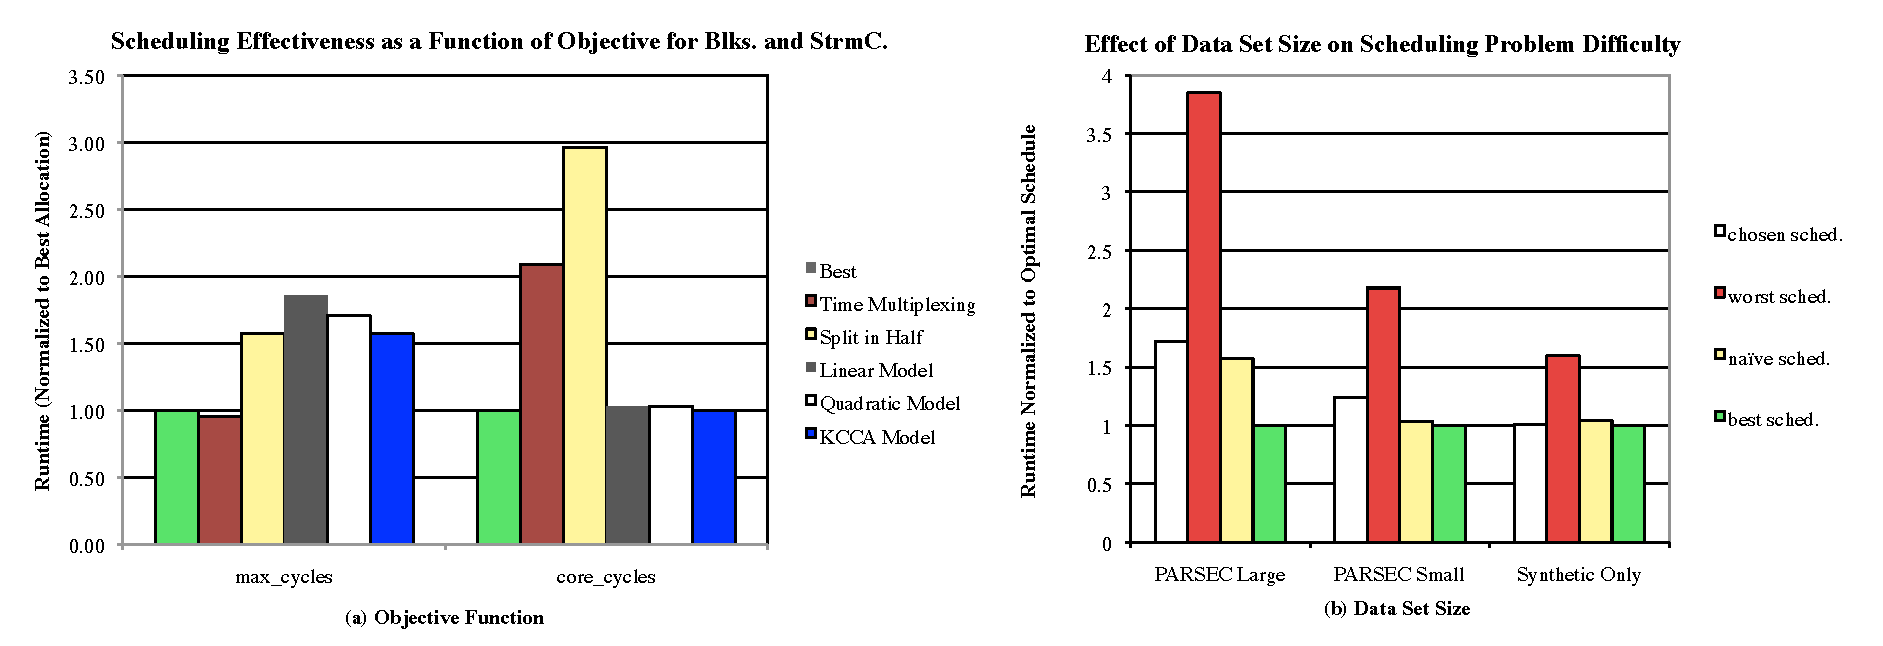
\includegraphics[width=1.0\textwidth]
        {Figures/case_study_outcome.pdf}}
        \caption{\label{fig:case_study_outcome}  (a) The performance
          of various scheduling methodologies and objective functions
          for one scheduling problem, normalized to the globally
          optimal schedule's performance.  The scheduler tries to
          minimize each objective function.  (b) The effect of
          benchmark size on the difficulty of the scheduling problem.
          The average chosen schedule performance, global worst case
          and naive scheduling case are normalized to the globally
          optimal schedule's performance for each dataset. The
          scheduling decision is Blackscholes vs. Streamcluster, the
          objective function is to minimize runtime.
 }
\end{figure*}

We found that predictive modeling has potential to successfully manage
some applications, depending on the scheduler's objective function.
For example, if the objective is to minimize energy, the approach
works quite well.  However, if the objective is to minimize the time
it takes to complete both applications, the naive baselines, such as
splitting the machine in half or time-multiplexing, often performed as
well or significantly better than model-based
allocation. Figure~\ref{fig:case_study_outcome}(a) presents an example
of these results. More importantly, our conclusions about the value of
model-based scheduling would have been different had we \emph{not}
simulated the entire execution of benchmarks, with large input sets,
for all possible allocations.

\begin{figure}[tb]
  \begin{center}
    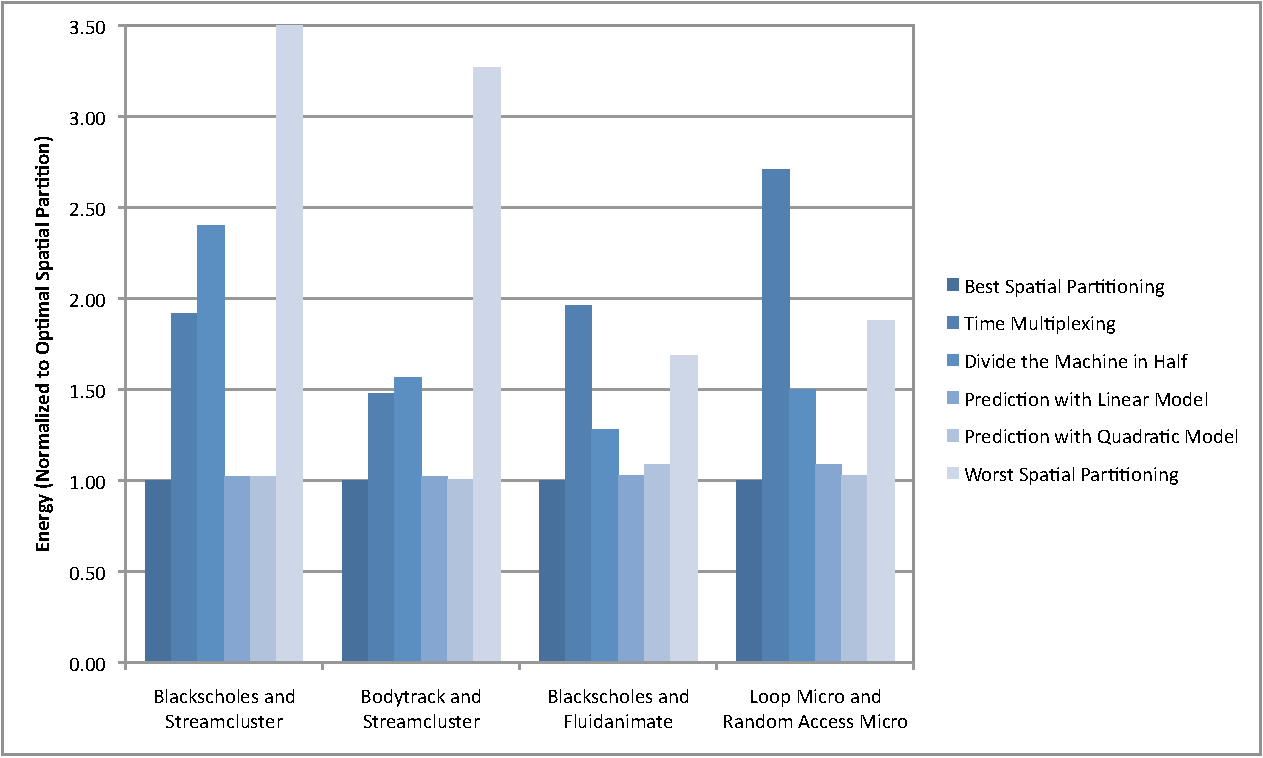
\includegraphics[width=\linewidth]{Figures/scheduling_results_energy.pdf}
  \end{center}
  \caption{Comparison of the effectiveness of different scheduling
    techniques normalized to our quadratic model-based approach.  The
    metric (sum of cycles on all cores + 10$\times$ sum of off-chip
    accesses) is a proxy for energy, so lower numbers are better.}
  \label{fig:scheduling_results}
\end{figure}




Figure~\ref{fig:scheduling_results} shows the results of our
scheduler's decisions based on the runtime performance data as
compared with several alternatives: the optimal allocation, naively
giving each application half of the machine, or time-multiplexing each
application across the entire machine.  

The time-multiplexing scheme
first runs the first application to completion and then runs the
second application to completion.  More fined-grained
time-multiplexing could lead to longer runtimes due to cache
interference effects and other context swap overheads.

We do no show results for the GPRS and KCCA as we found that they were extremely non-convex and as a result often produced very poor results when paired with our optimizer. The simple linear and quadratic models perform much better with only a small set of sample points and have significantly lower overhead.

The results
show that using runtime data to perform more intelligent scheduling
can lead to a significant savings in time and energy.  Our approach
beats naively dividing the machine by 65\% and time multiplexing by
100\% on average. Furthermore, it is within a few percent of optimal
every time.  The worst-case results show that the penalty for poor
decision making can be quite large, with an energy cost 3.25$\times$
greater than our allocation on average.

As the number of cores and other shared resources grows on chip, this
will increase the number of possible allocations, thereby widening the
performance gap between good and bad schedules.  Additionally, we
expect that much more code will be tuned for parallel execution, and
exhibit a greater variety of behaviors.  As a result, there will more
likely be disjoint resource requirements among applications available
to co-schedule.  We believe hardware measurement-based scheduling will
thus prove even more effective.


\subsection{\pacora Feasibility in a Real System}
Our static framework was designed to test the effectiveness of \pacora's model-based convex optimization for allocating resources.  We used it to experiment with the accuracy of different types of models and test the quality of the resource allocation decisions. Data is collected online by running application benchmarks on a recent x86 processor running Linux-2.6.36.  The measured data is processed using Python and then fed to MATLAB~\cite{matlab} to build the RTFs.  MATLAB uses the RTFs to make resource allocation decisions.  We compare performance of the chosen resource allocations with the actual measured performance of all possible resource allocations to test quality of the resource allocation decisions. We use CVX~\cite{cvx} in MATLAB to perform the convex optimization for building RTFs and making resource allocation decisions.  We chose this static approach because it let us test many applications, 44 in total, and many resource allocations rapidly.

\subsubsection{Platform}

To collect data, we use a prototype version of Intel's Sandy Bridge x86 processor that is similar to the
commercially available client chip, but with additional hardware
support for way-based LLC partitioning.
The Sandy Bridge client chip has 4 quad-issue out-of-order
superscalar cores, each of which supports 2 hyperthreads using
simultaneous multithreading~\cite{IntelRefManual:2011}.
%Each core has private \wunits{32}{KB} instruction and data caches, as well as a
%\wunits{256}{KB} private non-inclusive L2 cache.
The LLC is a 12-way
set-associative \wunits{6}{MB} inclusive L3 cache, shared among all
cores using a ring-based interconnect.
%All three cache levels are write-back.
The cache partitioning mechanism is way-based and works by modifying the
cache-replacement algorithm.  To allocate cache ways, we assign a subset of
the 12 ways to a set of hyperthreads, thereby allowing only those hyperthreads to replace data in those ways.

%Way allocations can be completely private,
%completely shared, or overlapping.  Although all cores can hit on data stored in
%any way, a core can only replace data in its assigned
%ways.   Data is not flushed when the way allocation changes.

We use a customized BIOS that enables the cache partitioning
mechanism, and run unmodified Linux-2.6.36 for all of our experiments.
To allocate cores, we use the Linux \texttt{taskset} command to pin applications to
sets of hyperthreads. The standard Linux scheduler performs the scheduling for applications within these containers of hyperthreads. For our experiments we consider each hyperthread to be an independent core. To minimize inter-application interference, we first assign both hyperthreads available in one core before moving on to the next core. For example, a 4-core allocation from \pacora represents 4 hyperthreads on 2 cores on the machine.

\subsubsection{Performance and Energy Measurement}

To measure application performance, we use the \texttt{libpfm}
library~\cite{Eranian:OLS06,Perfmon2}, built on top of the
\texttt{perf\_events} infrastructure in Linux, to
access available performance counters~\cite{Intel:Manual2012}.

To measure on-chip energy, we use the energy counters available on
Sandy Bridge to measure the consumption of  the entire socket and also
the total combined energy of cores, their private caches, and the
LLC. We access these counters using the Running Average Power Limit
(RAPL) interfaces~\cite{Intel:Manual2012}.  %The counters measure power
%at a $1/2^{16}$ second granularity.

%In addition, we use a FitPC external multimeter to measure at the wall socket the power
%consumed by the entire system, at a
%\wunits{1}{second} granularity.
%We correlate the wall power data with the data collected from the hardware energy counters
%using time stamps.  We observed less than one second of delay in these
%measurements consistently across all experiments.  Together, these
%mechanisms allow us to collect accurate energy readings over the
%entire course of an application's execution.

\subsubsection{Description of Workloads}

Our workload contains a range of applications from three different
popular benchmark suites: SPEC CPU 2006~\cite{SPEC2006},
DaCapo~\cite{dacapo}, and PARSEC~\cite{parsec}. We selected this set of applications to represent a wide variety of possible resource behaviors in order to properly stress \pacora's RTFs. We include some additional applications to broaden the
scope of the study, and some microbenchmarks to exercise certain
system features.

The \textbf{SPEC CPU2006} benchmark suite~\cite{SPEC2006} is a
CPU-intensive, single-threaded benchmark suite, designed to stress a
system's processor, memory subsystem, and compiler.  Using the
similarity analysis performed by Phansalkar \emph{et
al.}~\cite{Phansalkar:ISCA2007}, we subset the suite, selecting 4
integer benchmarks (\texttt{ astar}, \texttt{ libquantum}, \texttt{ mcf}, \texttt{ omnetpp}) and 4
floating-point benchmarks (cactusADM, calculix, lbm, povray).  Based
on the characterization study by Jaleel~\cite{Jaleel:TR2007}, we also
pick 4 extra floating-point benchmarks that stress the LLC: \texttt{ GemsFDTD},
\texttt{ leslie3d}, \texttt{ soplex} and \texttt{ sphinx3}.  When multiple input sets are
available, we pick the single \textit{ref} input indicated by~\cite{Phansalkar:ISCA2007}.

We include the \textbf{DaCapo} Java benchmark suite as a
representative of managed-language workloads. We use the latest 2009 release, which consists of a set of open-source, real-world
applications with non-trivial memory loads, and includes both client and
server-side applications.

The \textbf{PARSEC} benchmark suite is intended to be representative
of parallel real-world applications~\cite{parsec}. PARSEC
programs use various parallelization approaches, including data- and
task-parallelization. We use native input sets and the \texttt{ pthreads} version for all benchmarks, with the exception of
\texttt{freqmine}, which is only available in OpenMP.

We add four \textbf{additional parallel applications} to help ensure
we cover the space of interest: \texttt{ Browser\_animation} is a
multithreaded kernel representing a browser layout animation; \texttt{
  G500\_csr} code is a breadth-first search algorithm; \texttt{ Paradecoder} is a parallel
speech-recognition application that takes audio waveforms of human
speech and infers the most likely word sequence intended by the
speaker; \texttt{ Stencilprobe} simulates heat transfer in a fluid
using a parallel stencil kernel over a regular
grid~\cite{Kamil:Stencilprobe}.

We also add two \textbf{microbenchmarks} that stress the memory
system and cause increased interference between applications: \texttt{ stream\_uncached} is a memory and on-chip bandwidth hog
that continuously brings data from memory without caching it, while
\texttt{ ccbench} explores arrays of different sizes to determine the
structure of the cache hierarchy.

Using a performance characterization of the applications, we select a subset of the benchmarks that are representative of different possible responses to resource allocations in order to reduce our study to a feasible size.  Similar to \cite{Phansalkar:ISCA2007}, we use machine learning to select representative benchmarks.  We use a
hierarchical clustering algorithm~\cite{Phansalkar:ISCA2007} provided by the Python library \texttt{scipy-cluster} with the \textit{single-linkage} method.  The feature vector contains parameters to represent core scaling, cache scaling, prefetcher sensitivity and bandwidth sensitivity.  The clustering algorithm uses Euclidean distance between vectors to determine clusters.

The clustering results in 6 clusters representing the following (applications at the cluster center are listed in parenthesis):
 \begin{itemize}\itemsep0pt \parskip0pt \parsep5pt
\item no scalability, high cache utility, (\texttt{ 429.mcf})
\item no scalability, low cache utility, (\texttt{ 459.gems\-FDTD})
\item high scalability, low cache utility, (\texttt{ ferret})
\item limited scalability, high cache utility, (\texttt{ fop})
\item limited scalability, low cache utility, (\texttt{ dedup})
\item limited scalability, low bandwidth sensitivity, (\texttt{ batik})
\end{itemize}

%First, we create a feature vector for each application using the values in the previous subsection:
%1) execution time as we increase the number of threads; 2) execution time as we increase the LLC size; 3) prefetcher sensitivity; and 4) bandwidth sensitivity. All metrics are normalized to the interval $[0,1]$. In total we use vectors with 19 features ($7+10+1+1$).

%The clustering algorithm finds the smallest Euclidean distance of a pair of feature vectors and forms a cluster containing that pair. It continues selecting the next smallest distance between a pair and forms another cluster. Linkage criteria can be used to adjust cluster formation. The single-linkage we selected uses the minimum distance between a pair of objects in different clusters to determine the distance between them.

\subsubsection{RTF Experiments}
\begin{figure*}[!t]
	\begin{center}	
		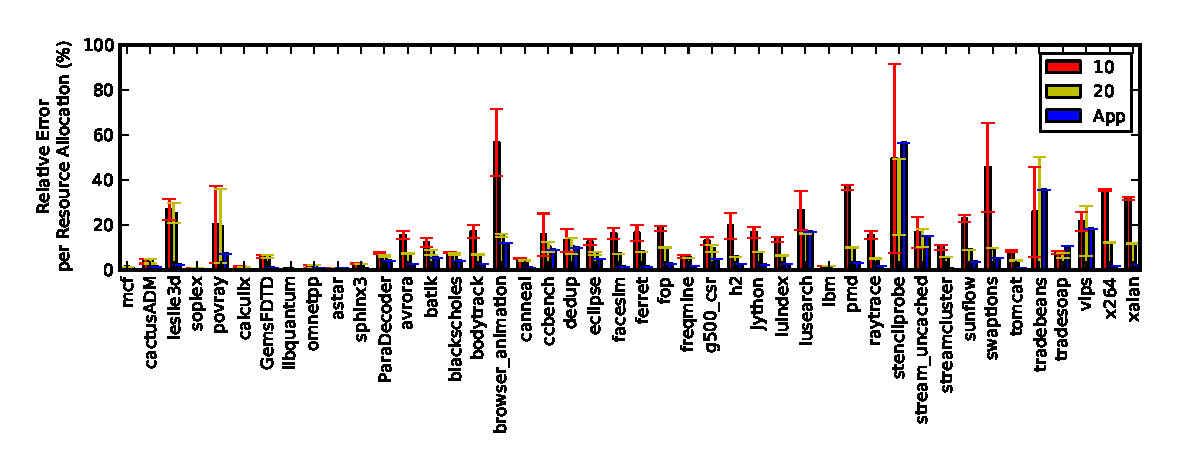
\includegraphics[bb=0 0 576 216,width=\textwidth]{Figures/model_accuracy.pdf}
		\caption{1-norm of relative error from RTF predicted response time compared to actual response time.  The actual response time is the median over 3 trials. 10 and 20 represent RTFs built with 10 and 20 training points respectively.  App represents the variability (average standard deviation) in performance of the application between the 3 trials.}
		\label{model_accuracy}
	\end{center}
\end{figure*}
To test the effectiveness of our RTFs in capturing real application behavior, we measure each of our 44 benchmarks running alone on the machine for all possible resource allocations of cache ways and cores.  Cores can be allocated from 1--8 and cache ways from 1--12 resulting in 96 possible allocations for each application.   We use a genetic algorithm design of experiments~\cite{bates-aes03} to select 10 and 20 of the collected allocations to build the RTFs.  We also experimented with building RTFs with more data points but found that they provided little improvement over 20~\cite{pacora_tr}.  We then use the model to predict the performance of every resource allocation and compare it with the actual measured performance (median value of 3 trials) of that resource allocation.  We built 3 different models from 3 trials and tested each of them against median measured value.

Figure~\ref{model_accuracy} shows the 1-norm of the relative error of the predicted response times per resource allocation for an RTF built with 10 training points and one built with 20.  The average error per point is 16\% for an RTF built with 10 training points and 9\% for an RTF built with 20 training points.  We also calculated the percentage variability (average standard deviation) for each resource allocation in the application between the 3 trials (shown as ``App'' in Figure~\ref{model_accuracy}).  The average variability is 9\%, so we can see that \pacora's RTFs are not much more inaccurate than the natural variation in response time in the application.  It is not for possible an RTF to be more accurate than the application variability, and we can also see that applications with higher variability result in RTFs with larger relative errors, (\emph{e.g.,} \texttt{stencilprobe}, \texttt{ tradebeans}).  Section~\ref{discuss} discusses application variability in more detail.

\subsubsection{Resource Allocation Experiments}
\begin{figure}[!t]
	\begin{center}	
		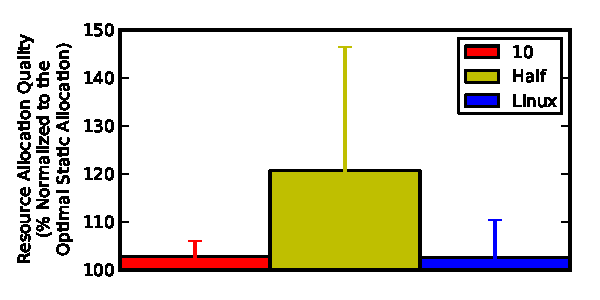
\includegraphics[bb=0 0 288 144,width=\columnwidth]{Figures/decision_quality.pdf}
		\caption{Resource allocation decisions for each pair of the cluster representative applications compared equally dividing the machine and a shared resources Linux baseline. Quality is measured is allocation performance divided by performance of the best possible allocation.}
		\label{decision_quality}
	\end{center}
\end{figure}


Using the RTFs built for the applications, we let \pacora make static resource allocations for all possible pairs of the cluster representative applications.  We then run an exhaustive study of all possible resource allocations for each pair on our Sandy Bridge-Linux platform, measure the performance, and compare it with the best performing, \emph{i.e.,} optimal, resource allocation.  We also compare this result to equally dividing the resources between the two applications and to sharing all of the resources using the standard Linux scheduler.

%how \pacora's decisions compared with the optimal allocation, equally dividing the machine, and the Linux baseline for each pair of the cluster representative applications.
Figure~\ref{decision_quality} shows these results for our 10 point RTFs. As we might expect, simple naive heuristics do not perform well, and dividing the machine in half is around 20\% slower than either \pacora or standard Linux.
 \pacora's resource allocations are 2\% from the optimal static allocation on average.  Using shared resources with the standard Linux scheduler performs similarly but with a higher standard deviation.  The shared resources comparison is interesting: while most of the time sharing resources can result in higher utilization, as the applications can dynamically take advantage of available resources, in some cases the interference between applications was so harmful to performance that on average optimal static partitioning performs slightly better.  As a result \pacora is able to provide performance comparable to Linux scheduling on shared resources with more predictable performance on average (lower worst cases).  Additionally, as the shown in the next Section, \pacora's resource allocation decisions do not need to be static, but can be made dynamically to adjust to the changing needs of the applications.
%These results indicate the \pacora is able to get a near optimal resource allocation and match the performance of the traditional Linux scheduler with more predictability.

\subsubsection{Effect of Model Accuracy on Decision Quality}

\begin{figure}[!t]
	\begin{center}	
%		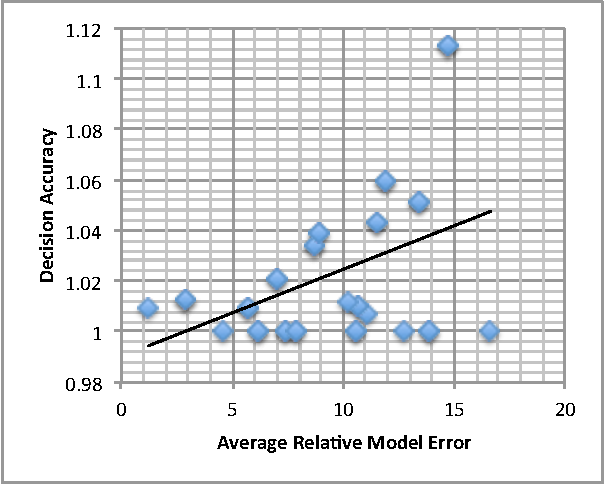
\includegraphics[width=0.9\textwidth]{cluster_decision_accuracy.pdf}
		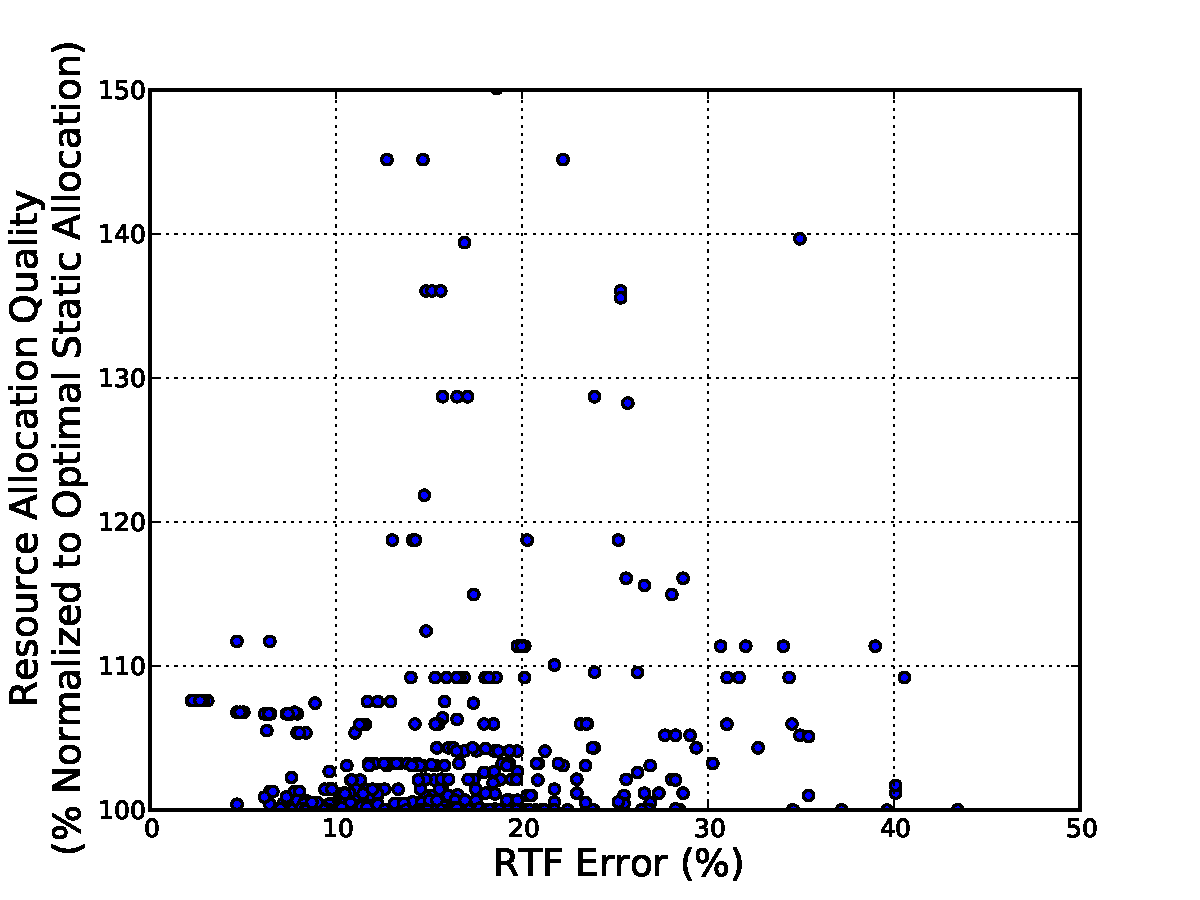
\includegraphics[bb=0 0 576 432,width=\columnwidth]{Figures/accuracy_quality.pdf}
		\caption{Effect of Model Accuracy on Decision Quality. The x axis represents the combined relative error of all RTFs used in the decision.}
		\label{accuracy_quality}
	\end{center}
\end{figure}


There are two main sources of challenges for \pacora's design: performance non-convexity and performance variability. 
The main concern with performance non-convexity and variability is their effects on the accuracy of the response time functions.  However, an important result we have found while evaluating \pacora is that model accuracy has less impact on the quality of resource allocation decisions than we anticipated.  When experimenting with possible models for the RTFs, we found that while some models were always a little too inaccurate and did degrade the performance of the resource allocation decisions, once a model crossed a certain threshold of accuracy then better models provided insignificant improvement in resource allocation decisions. Figure~\ref{accuracy_quality} shows the effect of model accuracy on the quality of the resource allocation decisions made using the RTF model in Equation~\ref{rtf_eq}.  Although there is a slight correlation between model accuracy and decision quality, many decisions with inaccurate models still result in near optimal allocations.  This effect enables \pacora's model-based design to be feasible in a noisy system with real applications.


\chapter{PACORA Implementation in a Manycore Operating System}\label{tess_design_ch}
In this chapter, we present our implementation of \pacora in \tess OS, a manycore research operating system \cite{tess_resource, tess, tess_dac, tess_audio, tess_gui}.  We give an overview of \tess and why we chose it for our implementation.  We then discuss the details for building RTFs online in the operating system.  Finally, we present our implementation of the resource allocator using an ADMM optimization method.



\section{Motivation}

We believe \pacora is applicable to many resource-allocation
scenarios from cloud computing to distributed embedded systems. For our initial prototype, we chose to study
\pacora implemented in a general-purpose operating system for client
systems, because we believe this scenario has some of the most
difficult resource allocation challenges: a constantly changing
application mix requiring low overhead and fast response times, shared
resources that create more interference among the applications, and
platforms that are too diverse to allow \emph{a priori} performance
prediction.

To evaluate \pacora's ability to make real-time decisions in a real operating system, we implemented it in an in-house research operating system, \tess. We chose to implement in \tess rather than Linux for three reasons:
 \begin{enumerate}\itemsep0pt \parskip0pt \parsep5pt
\item \tess separates resource allocation from scheduling, so is
  closer to the OS architecture assumed by \pacora
\item \tess allows resource revocation, enabling \pacora to dynamically reallocate resources
\item \tess implements additional resource partitioning mechanisms,
  letting \pacora manage  more resource types
\end{enumerate}

 Further, modifying a full-fledged production OS such as Linux to investigate new resources management schemas is complex and
 requires more implementation effort than developing for \tess's resource-centric OS\footnote{For example, the Earliest
 Deadline First (EDF) scheduler in \tess is only 800 lines of user-space code, contained in four files.  By contrast, support for
 EDF in Linux requires kernel modifications and substantially more code: the best-known EDF kernel patch for Linux, SCHED\_DEADLINE, has over 3500 modified lines in over 50 files.}.
We use the \tess implementation to test our implementations of the algorithms, measure the overhead and reaction times, and illustrate \pacora's ability to work in a real system. 

\section{\tess Overview}

This section briefly describes the key components of \tess OS~\cite{tess,tess_resource,tess_dac,tess_audio, tess_gui}.
The \tess kernel is a thin, hypervisor-like layer that provides support
for dynamic resource management.  It implements cell along with interfaces for user-level scheduling, resource
adaptation, and cell composition.  \tess currently runs on x86 hardware
platforms (\emph{e.g.,} with Intel's Sandy Bridge CPUs). 


\subsection{Cells}\label{sec:cell-model}

In \tess, resources are distributed to QoS domains called
\emph{cells}, which are explicitly parallel, light-weight, performance-isolated containers
with guaranteed, user-level access to resources. The software running within each cell has full
user-level control of the cell's resources.

\begin{figure}[tp]
%\vspace*{-0.2in}
\centering
%\rule{4cm}{3cm}
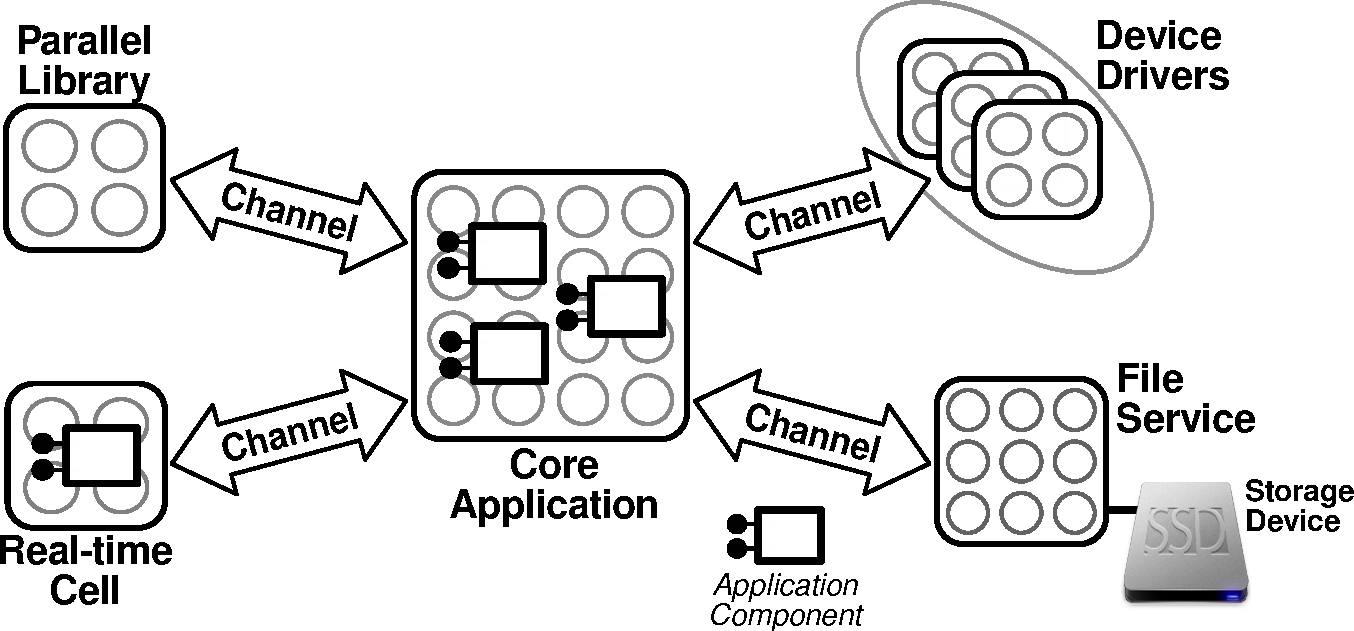
\includegraphics[width=1.0\columnwidth]{Figures/app-split-into-cells.pdf}
%\vspace*{-0.4in}
\caption{
Applications in \tess are created as sets of interacting components
hosted in different cells that communicate over channels.
Standard OS services (\eg the file service) are also hosted in cells and
accessed via channels.
}
\label{fig:app-split-into-cells}
%\vspace*{-0.15in}
\end{figure}

As depicted in Figure~\ref{fig:app-split-into-cells}, applications
in \tess are created by composing cells via \emph{channels}, which
provide fast, user-level asynchronous message-passing between cells.
Applications can then be split into performance-incompatible and
mutually distrusting cells with controlled communication. 


\tess OS implements cells on x86 platforms by partitioning resources
using \emph{space-time partitioning}~\cite{rushby99,lei03}, 
a multiplexing technique that divides the hardware into a sequence of
simultaneously-resident spatial partitions. 
Cores and other resources are
\textit{gang-scheduled}~\cite{gangsched1982,gangschedpatent}, so
cells provide to their hosted applications an environment that is very
similar to a dedicated machine.

\subsection{Resources and Services} \label{sec:soa} 
Partitionable resources include CPU cores, memory pages, and guaranteed
fractional services from other cells (\emph{e.g.,} a throughput reservation of 150~Mbps
from the network service).  
They may also include cache slices, portions of memory bandwidth, and fractions
of the energy budget, when hardware support is available
\cite{akesson07,lee08memqos,paolieri09,sanchez11}.

\tess also creates \emph{service cells} to encapsulate user-level device drivers and control devices.
Each service can thus arbitrate access to its
enclosed devices to offer service guarantees to
other cells. \tess treats the services
offered by the service cells as additional resources to be allocated to applications.

\tess currently has two such service cells implemented:
the \emph{Network Service}, which provides access to network adapters and
guarantees that the data flows are processed with the agreed levels of
throughput; and the \emph{GUI Service}, which provides a windowing system with
response-time guarantees for visual applications.  


\subsection{Resource Management and Scheduling} 

\begin{figure}[t]
\centering
%\rule{4cm}{3cm}
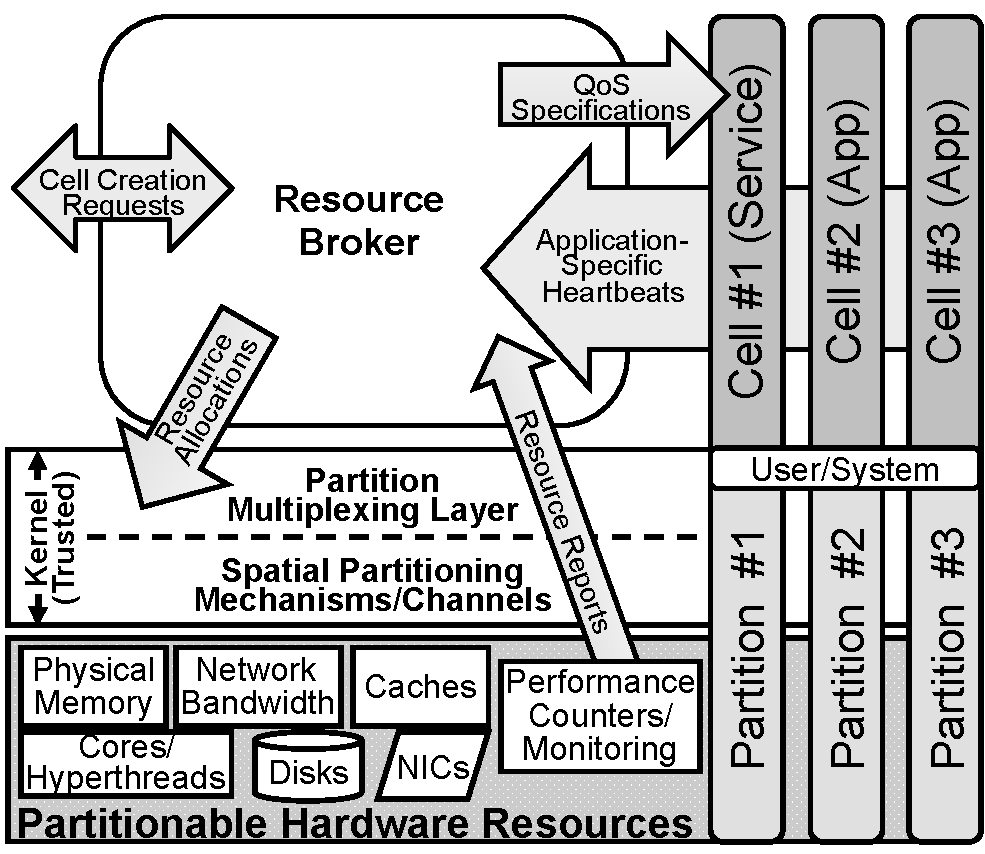
\includegraphics[width=0.885\linewidth]{Figures/NewPolicyFig-Tess}
%\vspace*{-0.1in}
\caption{
The \tess kernel implements \emph{cells} through \emph{spatial-partitioning}.
The \emph{Resource Broker} redistributes resources after consulting application-specific
\emph{heartbeats} and system-wide \emph{resource reports}.
}
\label{fig:tess-arch}
%\vspace*{-0.175in}
\end{figure}

\tess uses \emph{Two-level scheduling}~\cite{leiner07,ober08} %,tess10} 
to separate global decisions about allocation of resources \emph{to}
cells (\emph{first level}) from application-specific usage of resources
\emph{within} cells (\emph{second level}). 
Resource allocation occurs at a coarse time scale to allow time for cell scheduling decisions to become effective.

\subsubsection{Scheduling}
Scheduling within cells functions purely at the user-level, as
close to the \emph{bare metal} as possible, improving efficiency and
eliminating unpredictable OS interference.  \tess provides a framework for preemptive
scheduling, called \emph{Pulse}, enables customization and support for a wide
variety of application-specific runtimes and schedulers without
kernel-level modifications. 
The user-level runtime within each cell can be tuned for a specific
application or application domain with a custom scheduling algorithm.
Using Pulse, \tess provides pre-canned
implementations for TBB~\cite{tbb07} and a number of scheduling algorithms,
including Global Round Robin (GRR), Earliest Deadline First
(EDF), and Speed Balancing~\cite{juggle2013}.  
 
Pulse provides support for revoking resource from schedulers. If a core is removed, Pulse's auxiliary scheduler runs the cell's outstanding scheduler contexts in
a globally \emph{cooperative}, Round Robin manner; \ie a scheduler context runs
until it either completes and transitions into an application context, or yields
into Pulse, allowing other contexts to run. Additionally, the Pulse API provides callbacks to notify schedulers when the number of available cores
changes, enabling resource-aware scheduling. 

\subsubsection{Adaptive Resource Allocation} \label{sec:rsc-alloc}

Global resource allocation in Tessellation is performed by the \emph{Resource Broker}, as
shown in Figure~\ref{fig:tess-arch}. The Broker assigns 
resources to cells and communicates its allocation decisions to the kernel
and services for enforcement.  It reallocates resources,
for example, when a cell starts or finishes or when a cell significantly
changes performance.  The Broker can periodically adjust allocations; the
reallocation frequency provides a tradeoff between adaptability (to
changes in state) and stability (of user-level scheduling).

Rather than implementing a single policy, the Broker is resource allocation framework that supports
rapid development and testing of new allocation policies. We've implemented \pacora as a resource allocation policy inside the Resource Broker.
 
\section{\pacora in \tess}

\begin{figure}[t]
\centering
%\rule{4cm}{3cm}
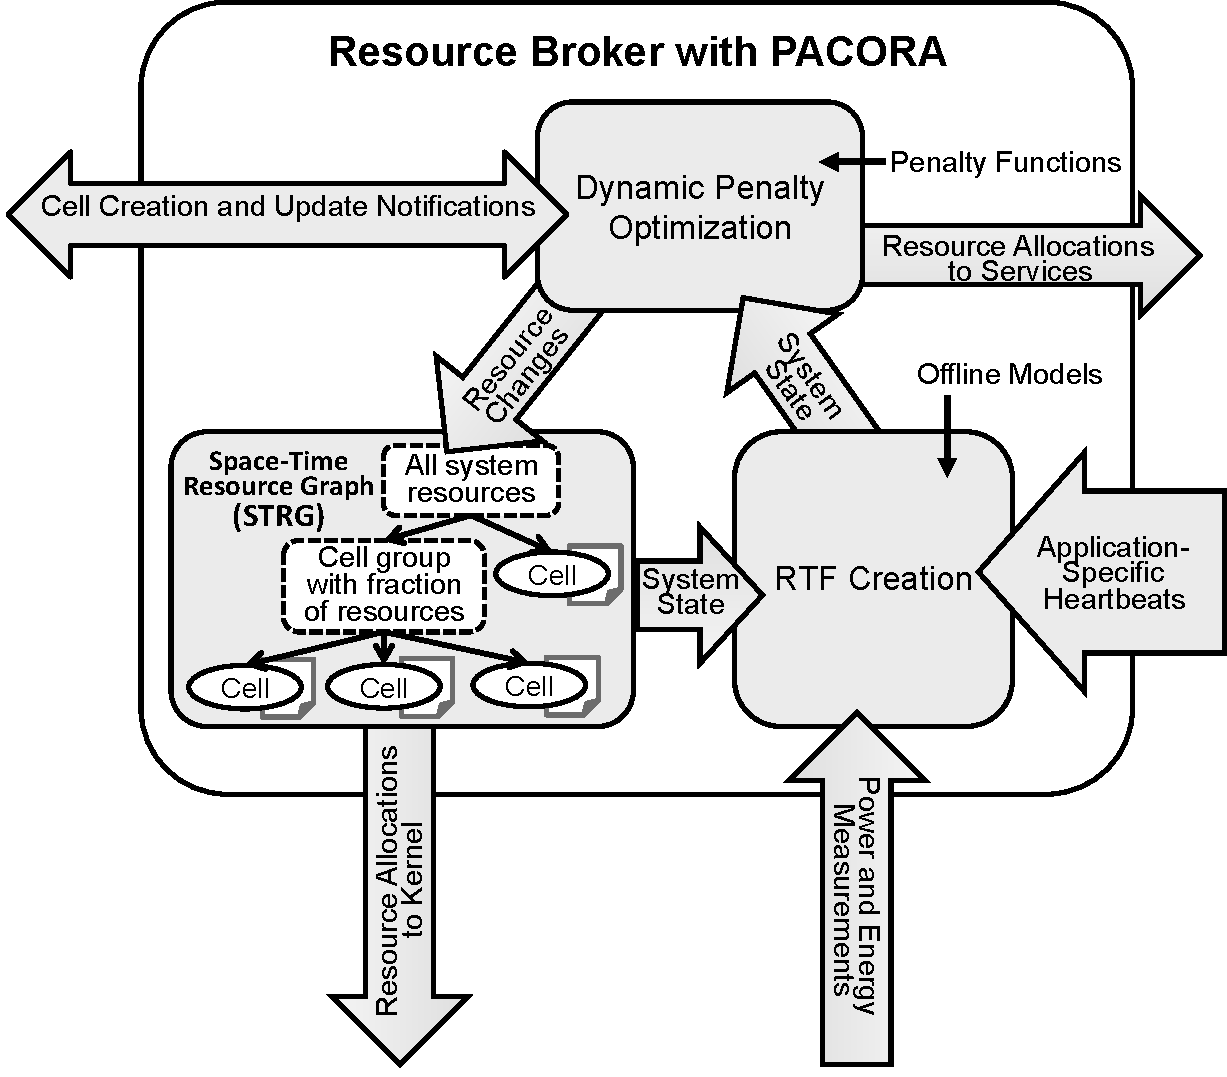
\includegraphics[width=0.885\linewidth]{Figures/pacora-in-tess}
%\vspace*{-0.1in}
\caption{
Overview of \pacora implementation in \tess.  \pacora leverages the existing Resource Broker interfaces to communicate with the cells, services, and kernel.  The RTF Creation and Dynamic Penalty Optimization modules contain \pacora's model creation and resource allocation functions.
}
\label{fig:pacora-in-tess}
%\vspace*{-0.175in}
\end{figure}

In this section, we provide details of \pacora's implementation in \tess's Resource Broker. Figure~\ref{fig:pacora-in-tess} shows the design. The Resource Broker runs in its own cell and communicates with applications and services through channels. \pacora leverages the existing Resource Broker interfaces to communicate with the cells, services, and kernel.  The RTF Creation and Dynamic Penalty Optimization modules contain \pacora's model creation and resource allocation functions and are described in Sections~\ref{rtf_creation} and~\ref{dyn_opt} respectively.

\subsection{Cell Creation}

When a cell is started, it opens its own channel with the Resource Broker and sends a cell creation message to register.
The registration message contains the deadline and slope for \pacora's penalty function and optionally, a starting RTF model.  The message format is shown below.  \pacora uses the \texttt{message\_type} field to determine how to unpack each of the message formats.

\begin{lstlisting}
typedef struct perf_function {

    char message_type;
    uint64_t runtime_target;
    float penalty_slope;
    float model_constants[MODEL_SIZE];

  } perf_func_t;  
                                                             
\end{lstlisting}

Ideally, penalty functions would be inferred by the system or provided by a
more trusted source than the applications themselves.  The simplest approach to implement this functionality in current operating systems would be to use an application's priority as the penalty slope and its interaction class~\cite{interaction_class} for the deadline. However, for our prototype the direct approach was straightforward to implement, and we believe does not detract from the validity of the resource allocation experiments\footnote{For cloud systems, this approach is, in fact, common practice: applications typically provide their resource requirements to the system.}.  


The Resource Broker also provides an interface for cells to update their penalty function or RTF while they are running, which we currently use to change RTF functions when an application changes phase or update the penalty function of application 0 when the computer changes operating mode (\ie from battery to power source).  The message formats for updating RTFs or Penalty Functions are shown below. 

\begin{lstlisting}
typedef struct penalty_update{

    char message_type;
    float penalty_slope;

} penalty_update_t;

typedef struct deadline_update{

    char message_type;
    uint64_t runtime_target;

} deadline_update_t;

typedef struct model_update{

    char message_type;
    float model_constants[MODEL_SIZE];

} model_update_t;
\end{lstlisting}

\subsection{Performance and Power Measurement}
Applications report their own measured response times to \pacora by periodically sending performance report messages, called \emph{heartbeats}~\cite{hoffmann2011}.  Messages may contain the value for a single heartbeat or heartbeats may be batched together.  The batch size is configurable, but is bounded by a maximum size, \texttt{MAX\_VALUES\_IN\_PERF\_REPORT}, set by the system.   The code below shows the heartbeat message format.

\begin{lstlisting}
typedef struct perf_report {

    char message_type;
    uint64_t data_values[MAX_VALUES_IN_PERF_REPORT];
    int32_t num_values;
    
} perf_report_t;
\end{lstlisting}

\pacora uses this information to build RTFs offline or online.  This process is described in Section~\ref{rtf_creation}.  As with the cell creation interface, it would be better for the system to directly measure application heartbeats rather than needing to trust the application's measurements.  However, measuring application-specific heartbeats in a general-purpose way is a challenging problem, and we chose not to address it in this work.  We instead focus exploring the value of resource allocation using application-specific measurements first.  Heartbeat measurement options are discussed further in Section~\ref{discuss}.

\tess provides a system call (show below) for \pacora to directly measure the system energy using the energy counters available on current x86 systems.  \pacora uses this information to build application 0's RTF.

\begin{lstlisting}
int sys_read_energy_counter(int32_t counter_id);
\end{lstlisting}

\subsection{Resource Allocation}
\pacora periodically optimizes the system penalty and produces resource allocations.  Details of this process are described in Section~\ref{dyn_opt}.  Allocation decisions are communicated to the kernel and services for enforcement.  Updates are sent to the kernel the update\_cells system call, which adjusts the Space-Time Resource Graph.  The function prototype for the system call is shown below.

\begin{lstlisting}
int sys_update_cells(cell_spec_t* updated_cell_specs, 
		    int32_t num_of_updated_cell_specs,
                     start_cell_params_t* new_cell_params,
                     int32_t* new_cell_ids,
                     int32_t num_of_new_cells);
\end{lstlisting}

The Resource Broker has a channel with each service to communicate allocations.  To update an allocation, \pacora sends a QoS Specification message to the service.  The function prototype to send the message is shown below.  The data field is service specific. 

\begin{lstlisting}
int change_allocation(int service_id, int cell_id, void *data,
 			size_t len, channel_gate_t* service_ch);
\end{lstlisting}

The Resource Broker design provides an adjustable reallocation frequency; the reallocation frequency provides a tradeoff
between adaptability (to changes in state) and stability (of user-level
scheduling).  

If \pacora is using offline models then it only makes sense to reallocate resources when a cell starts or finishes or when a cell updates its penalty function or RTF, since those are only points at which the inputs to the optimization change.  The exception to this is if optimization is terminated early for latency reasons, then each successive reallocation would move the allocations closer to optimal\footnote{We found early termination to be unnecessary since the complete optimization runs so quickly.  (This data is shown in Section~\ref{tess_eval}.)}. 

With online modeling reallocation could, in theory, be performed more frequently since the RTF functions can change as a cell runs.  However, the models will only change significantly as a result of an application phase change or application input change and so, in practice, it is similar to the offline modeling case\footnote{In the cloud, RTFs for applications such as web services may also change as a result of the incoming request load and thus require more frequent reallocation.}.

In our experiments (See Section~\ref{tess_eval}), we run \pacora continuously so that we can observe more resource allocation decisions. However, the allocations rarely change outside of the cases described above (\ie cell start/stop or phase/penalty change), so in practice it performs the same (in terms of resulting allocations) as if it were run periodically but with a higher overhead since it occupies at hardware thread for all time instead for only a single optimization at a time. 

\subsection{Application Requirements}
Our \tess implementation of \pacora requires minor modifications to applications\footnote{In addition to the modifications already required for an application to run on \tess}.  First, during the application initialization phase where the cell registers with \tess, a cell creation call must be added to open a channel with the Resource Broker and send the application's penalty function.  Second, the application must be modified to measure its response time and send these results to \pacora using the heartbeat interface.  For our applications, this simply required adding two timer calls and one message send.  Finally, if the system is using offline modeling and the application has multiple phases with different RTFs then an update RTF message must be sent when the application changes phase.  

These modifications are mostly a product of our prototype implementation decisions more than \pacora's fundamental design, and we hope that more advanced future implementations would eliminate the need to modify applications.   This is discussed further in Section~\ref{discuss}.

\section{RTF Creation}\label{rtf_creation}

There are many ways to collect the response time data for
applications. The user-level runtime scheduler is one possible source,
or the operating system could measure progress using performance
counters.  In our implementation, applications report their own
measured values; however, this solution was chosen simply as a way to
test the validity of the concept.  In a production operating system it
may not be a good idea because applications could lie about their
performance.  In a single-operator datacenter environment this might be less of a concern.

There are also many different possible moments to create response time functions.  RTFs could be created in advance and distributed with the application. This approach could make lots of sense for app stores since most of them cater to just a few platforms. RTFs could also be crowd-sourced and built in the cloud, which has the advantage making it easy to collect a diverse set of training points.  However, all of these approaches lack adaptability.  As a result, we have chosen to implement two solutions that collect data directly from the user's machine.  The first approach is to adapt to the system by collecting all of the training points at application install time and building the model then.  The most highly adaptive approach collects data continuously as the application runs, uses the data to modify the model training set, and rebuilds the model.  A hybrid approach may be the most effective: applications can begin with a generic model or crowdsourced and personalize it over time. The remainder of this section describes our model creation process in detail.

\subsection{Install Time Data Collection}
To create RTF models either at install time or online, we use a convex
least-squares approach described below.  At install time, we use a
genetic algorithm, Audze-Eglasis Design of
Experiments~\cite{bates-aes03}, to select the resource allocation vectors to use
for training.  The application is run with each resource vector for a configurable number of heartbeats to record the response time.  We average the response times collected for an allocation and use that result as the response time for the model\footnote{The \tess OS and our applications both have very little variability so average works fine for our purposes; however, Section~\ref{discuss} discusses why average may not be the right choice in other situations.}.  These vectors and their response times are fed into the
convex least-squares algorithm. Offline models are built entirely from this install time data.  Online modeling uses the response times measured as the application runs in the models, but it could also start with a model built at install time.

\subsection*{Least-Squares Minimization}
After enough measurements, the model parameters $w$ of an application's RTF $\tau$ (shown in Equation~\ref{rtf_eq})
can be discovered by solving an over-determined linear system $t=Dw$,
where $t$ is a column vector of actual response times measured for the application
and $D$ is a matrix whose $i$th row $D_{i,*}$ contains the corresponding resource vector.
Estimating $w$ is relatively straightforward: we've implemented a least-squares solution using
\emph{QR factorization}~\cite{GoVL} of $D$ to determine the $w$ that minimizes the \emph residual error of
$\|Dw - t\|^2_2 =  \|Rw - Q^Tt\|^2_2$.
The solution proceeds as follows:
\begin{eqnarray*}
t     &=& Dw  - \varepsilon    \\
      &=& QRw - \varepsilon    \\
Q^Tt  &=& Rw  - Q^T\varepsilon
\end{eqnarray*}

The individual elementary orthogonal transformations, \emph{e.g.,} Givens rotations,
that triangularize $R$ by progressively zeroing out $D$'s sub-diagonal elements are simultaneously applied to $t$.
The elements of the resulting vector $Q^Tt$ that correspond to zero rows in $R$ comprise $-Q^T\varepsilon$.
Since $Rw$ exactly equals the upper part of $Q^Tt$, the upper part of $Q^T\varepsilon$ is zero. The residual error for the $t_i$
can be found by premultiplying $Q^T\varepsilon$ by $Q$.

This formulation assumes a model norm $p = 1$. If a different model norm $p$ is desired, such as $p = 2$, we could first square each measurement in $t$
and each reciprocal bandwidth term in $D$ and then follow the foregoing procedure.
The elements of the result $w$ will be squares as well, and the 2-norm of the difference in the squared quantities will be minimized\footnote{This is not the same as minimizing the 4-norm; what is being minimized is $1/2\|\mbox{diag}(Dww^TD^T - tt^T)\|^2_2$.}.

\subsection*{Incremental Least-Squares}
As resource allocation continues, more measurements will become available to augment $t$ and $D$.
Moreover, older data may poorly represent the current behavior of the application.  Rather than periodically rebuilding the RTFs functions completely, we've implemented an incremental approach described below to replace old data and efficiently update RTFs with each new data value.

What is needed is a factorization $\tilde{Q}\tilde{R}$ of a new matrix $\tilde{D}$
derived from $D$ by dropping a row,
and adding a row.
Corresponding elements of $t$ are dropped and added to form $\tilde{t}$.

The matrices $\tilde{Q}$ and $\tilde{R}$ can be generated by applying Givens rotations
as described in Section 12 of \cite{GoVL} to \emph{downdate} or \emph{update} the factorization
much more cheaply than recomputing it \emph{ab initio}.
The method requires retention and maintenance of $Q^T$ but not of $D$.
Every update in \pacora is preceded by a downdate that makes room for it.
Downdated rows are \emph{not} always the oldest (bottom) ones, but
an update always adds a new top row.
For several reasons, the number of rows $m$ in $R$
will be at least twice the number of columns $n$.
Rows selected for downdating will always be in the lower $m - n$ rows of $R$,
guaranteeing that the most recent $n$ updates are always part of the model.


To guarantee convexity of the RTF, the solution $w$ to $t \approx QRw$ must have no negative components.
Intuitively, when a resource is associated with more than a single $w_j$
or when the measured response time increases with allocation then negative $w_j$ may occur. \emph{Non-negative Least-Squares} problems (NNLS) are common linear algebra, and there are several well-known techniques~\cite{ChPl}.
However since \pacora's online model maintenance calls for
incremental downdates and updates to rows of $Q^T$, $Q^Tt$ and $R$,
the NNLS problem is handled with a scheme
based on the \emph{active-set} method\cite{LaHa} that
also downdates and updates the \emph{columns} of $R$ incrementally,
roughly in the spirit of Algorithm~3 in~\cite{LuDu}.
However, \pacora's algorithm cannot ignore downdated columns of $R$
because subsequent \emph{row} updates and downdates must have due effect
on these columns to allow their later reintroduction via column updates as necessary.
This problem is solved by leaving the downdated columns in place,
skipping over them in maintaining and using the QR factorization.

The memory used in maintaining a model with $n$ weights is modest, $24n^2 + 21n + \textrm{O}(1)$ bytes.
For $n = 8$ this is under 2 KB, fitting nicely in L1 cache.
Our NNLS implementation takes \SI{4}{\micro\second} per update-downdate pair in \tess.  The sections below describe the our row and column update/downdate, rank preservation, and outlier minimization algorithms in more detail.


\subsubsection{Row Update and Downdate}

Downdating makes an instructive example. A row downdate operation applies
a sequence of Givens rotations to the rows of $Q^T$.
The rotations are calculated to set every $Q^T_{i,dd}$, $i \neq dd$ to zero.
In the end only the diagonal element $Q^T_{dd,dd}$ of column $dd$ will be nonzero.
Since $Q^T$ remains orthogonal, the non-diagonal elements of row $dd$ will also have been zeroed automatically
and the diagonal element will have absolute value 1.
These same rotations are concurrently applied to the elements of $Q^T t$ and to the rows of $R$ $(= Q^T D)$
to reflect the effect that these transformations have on $Q^T$.

It is crucial to select pairs of rows and an order of rotations that preserves the upper triangular structure of $R$
while zeroing all but the diagonal entry of the chosen column $dd$ of $Q^T$.
Since $dd$ is always below the diagonal of $R$ it initially will contain only zeros.
It is therefore sufficient to rotate every non-$dd$ row with row $dd$, proceeding from bottom to top.
The first $m - n - 1$ rotations will keep row $R_{dd,*}$ entirely zero,
and the remaining $n$ rotations will introduce nonzeros in $R_{dd,*}$ from right to left.
The effect on $R$ will be to replace zero elements by nonzero elements only within row $dd$.
At this point, except for a possible difference in overall sign, $R_{dd,*} = D_{dd,*}$.

Now the rows from 0 down through $dd$ of the modified matrices $Q^Tt$ and $R$ and both the rows and columns of the modified $Q^T$
are circularly shifted by one position, moving row $dd$ to the top (and column $dd$ of $Q^T$ to the left edge).
The following is the result:
\begin{displaymath}
\begin{array}{lll}
    \left[\begin{array}{cc}
      \pm1  &  0 \\
      0     &  \tilde{Q}^T
   \end{array}\right]
   \left[\begin{array}{c}
      t_{dd} \\
      \tilde{t}
   \end{array}\right]
   &=&
   \left[\begin{array}{c}
      \pm D_{dd,*} \\
      \tilde{R}
   \end{array}\right] w
   \\
   \\
   &-&
   \left[\begin{array}{cc}
      \pm1  &  0 \\
      0     &  \tilde{Q}^T
   \end{array}\right]
   \left[\begin{array}{c}
      \varepsilon_{dd} \\
      \tilde{\varepsilon}
   \end{array}\right]
\end{array}
\end{displaymath}
The top row has thus been decoupled from the rest of the factorization and may either be deleted or updated with new data.

The update process more or less reverses these steps, adding a new top row to $R$ and $t$ and a row and column to $Q^T$.
Then $R$ is made upper triangular once more by a sequence of Givens rotations that zero its sub-diagonal elements
(formerly the diagonal elements of $\tilde{R}$) one at a time.
These rotations are applied not just to $R$ but also to $Q^Tt$ and of course to $Q^T$ itself.

\subsubsection{Rank Preservation}

If care is not taken in downdating $R$, its rows may become so linearly dependent,
perhaps from repetitive resource allocations,
that determining a unique $w$ is impossible.
The rank of $R$ depends on both the resource optimization trajectory and the
choices made in the row downdate-update algorithm.
\pacora exploits the latter idea and simply avoids downdating any row that will make $R$ rank-deficient.

Deciding in advance whether downdating a row of $R$ will reduce its rank
is equivalent to predicting whether one of the Givens rotations, when applied to $R$,
will zero or nearly zero a diagonal entry of $R$.
This is particularly easy to discover because $dd$, the row to be downdated, is initially all zeros in $R$,
\emph{i.e.} in the lower part of the matrix.
In this situation a diagonal entry of $R$, $R_{i,i}$ say, will be compromised if and only if the
cosine of the Givens rotation that involves rows $dd$ and $i$ is nearly zero.
The result will be an interchange of the zero in $R_{dd,i}$ with the nonzero diagonal element $R_{i,i}$.
$R_{dd,i}$ is zero before the rotation because
$R$ was originally upper triangular and prior rotations only involved row subscripts greater than $i$.

\pacora keeps track of the sequence of values in $Q^T_{dd,dd}$ without actually changing $Q^T$
so that if the downdate at location $dd$ is eventually aborted there is nothing to undo.
It is also possible to remember the sines and cosines of the sequence of rotations
so they don't have to be recomputed if success ensues.
A rank-preserving row to downdate will always be available as long as $R$ is sufficiently ``tall''.
Having at least twice as many rows as columns is enough since the number of available rows to downdate
matches or exceeds the maximum possible rank of $R$.

\subsubsection{Column Update and Downdate}

The active-set NNLS method is based on the idea that since the only constraints are variable positivity
then for all components either the variable or its gradient will be zero at a solution point; see~\cite{BoVa}, page~142.
The active set, denoted by \textbf{Z}, comprises the column subscripts $j$ for which the variable $w_j$ is zero and the gradient $v_j$ is positive. If a column $j$ not currently in \textbf{Z} happens to acquire a negative $w_j$ after a back-solve, $w_j$ is zeroed,
$j$ is moved into \textbf{Z} and column $j$ is downdated in $R$, thereby making the gradient positive.
Conversely, if a column already in \textbf{Z} happens to acquire a negative gradient $v_j$ it is removed from \textbf{Z} and updated in $R$,
allowing it to further reduce the value of the objective function.

After initial acquisition of data and $QR$ factorization, each step of \pacora's NNLS algorithm
combines incremental row and column downdates and updates as follows:

\begin{pseudocode}{IncrementalNNLS}{t_0,d_0}
\LOCAL{R,Q^T,Q^Tt,w,v,idx,d,u,done}                              \\
R,Q^T,Q^Tt \GETS \textsc{DndtRow}(R,Q^T,Q^Tt,idx)           \\
R,Q^T,Q^Tt \GETS \textsc{UpdtRow}(t_0,d_0,R,Q^T,Q^Tt,idx)     \\
w \GETS \textsc{BackSolve}(R,Q^Tt,idx)                          \\
v \GETS \textsc{Gradient}(R,Q^Tt,idx)                    \\
\REPEAT
  done \GETS \TRUE                                              \\
  d \GETS \arg\min(w)                                          \\
  \IF w_d < 0 \THEN                                            \\
  \BEGIN
    done \GETS \FALSE                                         \\
    R,Q^T,Q^Tt,idx \GETS \textsc{DndtCol}(R,Q^T,Q^Tt,idx,d)   \\
    w \GETS \textsc{BackSolve}(R,Q^Tt,idx)                    \\
    v \GETS \textsc{Gradient}(R,Q^Tt,idx)              \\
  \END                                                        \\
  u \GETS \arg\min(v)                                         \\
  \IF v_u < 0 \THEN                                           \\
  \BEGIN
    done \GETS \FALSE                                         \\
    R,Q^T,Q^Tt,idx \GETS \textsc{UpdtCol}(R,Q^T,Q^Tt,idx,u)     \\
    w \GETS \textsc{BackSolve}(R,Q^Tt,idx)                    \\
    v \GETS \textsc{Gradient}(R,Q^Tt,idx)              \\
  \END                                                        \\
\UNTIL done                                                   \\
\RETURN{w,v}                                                  \\
\end{pseudocode}

The set \textbf{Z} and its complement \textbf{P} are implemented as an index $idx$
containing a vector of the column subscripts comprising \textbf{P} in increasing order
followed by the column subscripts of \textbf{Z} in increasing order;
$idx$ also contains an offset defining the beginning of \textbf{Z} in the vector.
For example, if columns 1, 3, and 4 are in \textbf{Z} and columns 0, 2, and 5 are in \textbf{P}
then the resulting vector is [0 2 5 1 3 4] and the offset is 3.
Since the offset is just the size of the set \textbf{P} it is naturally called $p$.

Regaqrdless of status, columns are left in place in $R$
The columns of $R$ belonging to \textbf{P} are denoted by $R^p$ and those in \textbf{Z} by $R^z$.
The updating or downdating of a column only involves modifying the index $idx$ to redefine \textbf{P} and \textbf{Z} and then
applying Givens rotations to the rows of $R$ to restore $R^p$ to upper triangular form.

When a column indexed by $d$ in $R^p$ is downdated because $w_d < 0$, that column is moved from \textbf{P} to \textbf{Z} in $idx$.
To restore $R^p$ to upper triangular form, Givens rotations are applied to $R$ at rows $R_{d,*}$ and $R_{k,*}$
where $d < k < p$. The row subscripts $k$ are used in decreasing order from $p-1$ down to $d+1$,
and each rotation zeros the subdiagonal element in $R^p$ of the column indexed by $k$.
As usual, these rotations are also applied to $Q^T$ and $Q^Tt$.
The result in $R^z$ is a ``spike'' of nonzeros in the column that was moved;
it can eventually extend to the bottom of $R$ as \emph{row} updates occur.

Column movements from \textbf{Z} to \textbf{P} are based on the gradient $v$ of the objective function, namely
\begin{eqnarray*}
v &=& 1/2\nabla\|Dw - t\|^2_2 \\
  &=& D^T(Dw - t)             \\
  &=& R^TQ^T(QRw - t)         \\
  &=& R^T(Rw - Q^Tt)          \\
  &=& R^T(-Q^T\varepsilon).
\end{eqnarray*}
If for some column in \textbf{Z} the inner product of the corresponding spiked row in $R^T$ and $-Q^T\varepsilon$ is negative,
the column subscript must be moved to \textsc{P}.
Updating $R^p$ reverses the downdating steps by zeroing the spike via a sequence of Givens rotations on $R$
between adjacent pairs of rows, starting at the bottom and ending at $m,m+1$ where $m$ is the position of the new column in $idx$.
These rotations conveniently extend the columns to the right of $m$ in $R^p$ by one,
thus restoring $R^p$ to upper triangular form. Once again, the rotations are also applied to $Q^T$ and $Q^Tt$.

A new gradient computation and new back-solve for $w$ are clearly necessary after either downdates or updates to columns of $R$.




\subsubsection*{Outliers and Phase Changes}


Some response time measurements may be ``noisy'' or even erroneous.
A weakness of least-squares modeling is the high importance it gives to outlying values.
On the other hand, when an application changes phase it is important to adapt quickly,
and what looks like an outlier when it first appears may be a harbinger of change.
What is needed is a way to discard either old or outlying data
with a judicious balance between age and anomaly.

The downdating algorithm accomplishes this by weighting the errors in $\varepsilon = Q(Q^Tt - Rw)$
between the predicted response times $\tau$ and the measured ones $t$ by a factor
that increases exponentially with the age $g(i)$ of the error $\varepsilon_i$.
Age can be modeled coarsely by the number of time quanta of some size since the measurement;
\pacora simply lets $g(i) = i$.
The weighting factor for the $i$th row is then $\eta^{g(i)}$ where $\eta$ is a constant somewhat greater than 1.
The candidate row to downdate is the row with the largest weighted error, \emph{i.e.,}
$dd = \arg\max_i |\varepsilon_i| \cdot \eta^{g(i)}$ and that does not reduce the rank of $R$.



\section{Dynamic Penalty Optimization}\label{dyn_opt}

%IV.	Dynamic Optimization
%	a.	Gradient Descent w/ Backtracking Search
%		i. boundary conditions clean up
%	b.	Dealing with Fractional Results

\pacora's penalty optimization algorithm dynamically decides resource allocations. The algorithm can be run periodically, when applications start or stop, when an application changes phase or when the system changes operating scenarios.  One of the advantages of convex optimization is that it enables fast, incremental solutions.  As shown in our experiments, the algorithm can terminate earlier to decrease overhead and still be moving towards an optimal solution as it runs.  %However we found in our implementation that the algorithm was fast enough to run to completion every time. 

Convex optimization is simplest when it is unconstrained, so we reformulated \pacora's construction to be unconstrained.
Extending the response time model functions to all of $\Re^n$
moves the requirement that allocations must be positive into the objective function,
and introducing application 0 for slack resources turns the affine inequalities into equalities:
\begin{eqnarray*}
& \makebox[1in][r]{Minimize}   & \sum_{p\in P} {\pi_p(\tau_p(a_{p,1}\ldots a_{p,n}))}  \\
& \makebox[1in][r]{Subject to} & \sum_{p\in P} a_{p,r} = A_r, r = 1,\ldots n           \\
\end{eqnarray*}

The only remaining constraints are those on the $a_{p,r}$.
These can be removed by letting the $a_{p,r}$ be unbounded above for $p \neq 0$
and changing the domain of $\tau_0$  to be the whole resource allocation matrix.
The definition of $\tau_0$ might take the form
\begin{eqnarray*}
\tau_0 &=& \sum_r \Delta_r \sum_{p \neq 0} a_{p,r}     \\
       &=& \sum_r \Delta_r (A_r - a_{0,r})
\end{eqnarray*}
where $\Delta_r$ is the (constant) power dissipation of one unit of resource $r$.
However, if any of the allocations $a_{0,r}$ turns out to be negative then $\tau_0$  should instead return the value $+\infty$.
%This modification of the objective function transforms the resource allocation problem
%to unconstrained convex optimization.  

The penalty optimization algorithm used in \pacora is gradient descent via backtracking line search along the negative gradient direction \cite{BoVa}.
This algorithm rejects and refines any step that yields insufficient relative improvement in the objective function,
so infinite values from infeasible allocations will automatically be avoided by the search.
The negative gradient $-\nabla\pi$ of the overall objective function $\pi$
with respect to the resource allocations $a$
is computed analytically from the response time models and penalty functions.
When a component of this overall gradient is negative,
it means the penalty will be reduced by increasing the associated allocation if possible.
The gradient search at the boundaries of the feasible region
must ignore components that lead in infeasible directions;
these can be detected by noting whether for some $p$ and $r$, $a_{p,r} = 0$ with $(-\nabla\pi)_{p,r} > 0$.
In such cases, the associated step component is set to zero.

We added an additional optimization to move along boundaries more rapidly in the scenario when a completely allocated resource had a large gradient.  We scale all the allocations of that resource type down to satisfy resource constraint while leaving the allocations of other resources untouched.

The rate of convergence of gradient descent depends on how well the sub-level sets of the objective function
are conditioned (basically, how ``spherical'' they are).
Conditioning will improve if resource allocation units are scaled to make their relative effects similar.
For example, when compared with processor allocation units,
memory allocation units of 4 MB are probably a better choice than 4 KB.
In addition, penalty function slopes should not differ by more than perhaps two orders of magnitude. If these measures prove insufficient, stronger preconditioners can be used. Our implementation conditions all resource allocations to be in the range of 0-100.

%\begin{figure}[!t]
%	\begin{center}	
%		\includegraphics[bb=0 0 576 432,width=\columnwidth]{opt_time.pdf}
%%		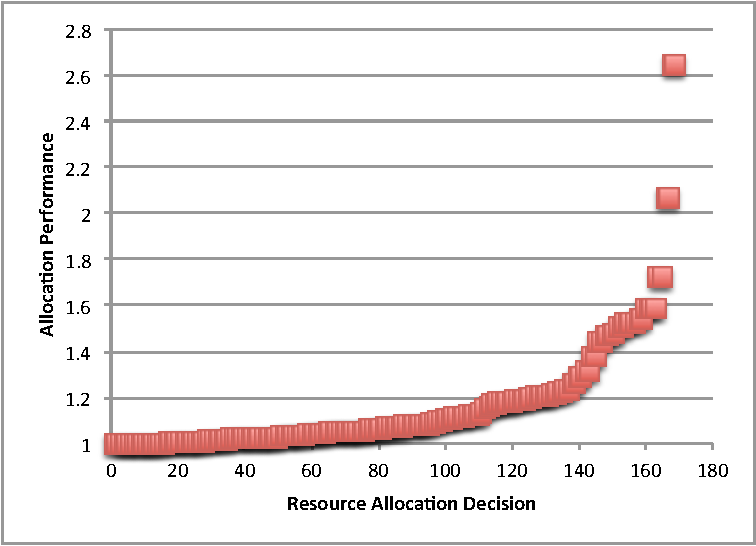
\includegraphics[width=.45\textwidth]{parsec_decision_points.pdf}
%		\caption{Performance of our penalty optimization algorithm}
%		\label{optimization_perf}
%	\end{center}
%\end{figure}


%Figure~\ref{optimization_perf} shows performance of the penalty optimization algorithm implemented in \tess.  

%For our video conferencing scenario the average runtime is \fix{x} and then worst case runtime is \fix{y}.  \fix{explain where the variance comes from}


\subsection{Resource allocation}

We follow the notation in \S 7.3 of Boyd et al. \cite{ADMM},
from which this material is taken almost verbatim.
We have $n$ resources and $N$ participants.
We let $x_i \in \reals^n_+$ denote the vector of resources 
that participant $i$ consumes.  
The (vector of) total resource consumption is then $x_1 + \cdots + x_N$;
for future use we let $z$ denote the average resource
usage per participant, \ie, the total divided by $N$.
Participant $i$ has a cost function $f_i:\reals^n \to \reals \cup
\{\infty\}$, where
$f_i$ is convex.  We let $f_i$ take on the value $+\infty$ to encode
constraints on the resource allocation.

The total cost function is
\[
f_1(x_1) + \cdots + f_N (x_N) + g(Nz),
\]
where $g: \reals^n \to \reals \cup \{+\infty\}$ is the cost
of consuming a total amount of resources (including any limits on total
available resources).
Note that the first $N$ terms are the costs associated with the
participants, and the last term is the cost of providing the total
resources.
The problem is to choose the allocations $x_i$ to minimize the total cost,
which is a convex optimization problem \cite{BoVa,ADMM}.

We will solve this problem using the \emph{sharing ADMM algorithm}
from \cite{ADMM}:
\begin{eqnarray*}
x_i^{k+1} &:=&  \argmin_{x_i} \left( f_i(x_i) + (\rho/2)
\|x_i-x_i^k+\overline x^k-z^k+u^k\|^2_2\right)\\
z^{k+1} &:=&  \argmin_{z} \left( g(Nz) + (N\rho/2)
\|z - u^k - \overline x^{k+1} \|_2^2 \right)\\
u^{k+1} &:=&  u^k + \overline x^{k+1}- z^{k+1}.
\end{eqnarray*}
Here $\rho>0$ is an algorithm parameter,
$k$ is the iteration number,
and $\overline x^k$ is the average of the consumption vectors
$x^k_1, \ldots, x^k_N$.
We interpret $x_i^k$ as the (proposed) resource consumption of 
participant $i$,
$z^k$ as the (proposed) average resource consumption,
and $u^k$ as a dual variable, all at iteration $k$.
This algorithm converges to an optimal allocation,
and $(1/\rho)u^k$ converges
to the optimal dual variables (prices) for the resources.

The $x$-update can be carried out in parallel, for $i=1, \ldots, N$.
Each participant, in each iteration, must minimize a function of the form
\[
f_i(x_i) + (\rho/2) \|x_i - v\|_2^2,
\]
\ie, each participant evaluates a proximal operator; see
\cite{ProxAlgs}.

The $z$-update step requires
gathering $x_i^{k+1}$ to form the averages, and then solving a problem
with $n$ variables.  This step is also a proximal evaluation.

After the $u$-update, the new value of $\overline x^{k+1}-
z^{k+1}+u^{k+1}$ is scattered to the subsystems.

\subsection{Excess latency minimization}

We now specialize to a latency minimization problem,
where the participants are processes and the participant costs 
are related to their latencies.

\subsubsection{Participants}

The latency (time delay) of each process depends on the 
resources allocated to the process.
Our model of the latency of process $i$ is
\[
l_i(x_i) = a_i + \sum_{j=1}^n (w_i)_j/(x_i)_j
\]
for $x_i >0$, and $+\infty$ otherwise, where $a_i \in \reals_+$ and 
$w_i \in \reals_{++}^n$ are given latency model parameters.
The participant cost is given by
\[
f_i(x_i) = \alpha_i (l_i(x_i) - t_i)_+,
\]
where $\alpha >0$ is a parameter and $t_i$ is a target latency.
Note that $l_i(x_i)-t_i$ is the excess latency.

We commment that the target latency in the cost function here is
probably not the actual target latency for our system, but rather
a target latency below which we do not impose a cost.  If the system
specification is for process $i$ to have (to the extent possible) latency
not exceeding $T_i$, then we might choose, for example, $t_i= 0.9T_i$.
In this case, there is no latency cost as long as the process latency is
less than the specification latency, with at least $10\%$ margin.

In each iteration of the sharing algorithm, 
we need to evaluate the proximal operator of $f_i$.
To simply notation, we drop the subscript $i$ and consider one
participant.
We need to minimize
\[
\alpha \left(a + \sum_{j=1}^n w_j/x_j - t\right)_+ + 
(\rho/2)\sum_{j=1}^n (x_j - v_j)^2
\]
over $x_j\geq 0$.
Note that we can combine $\alpha$ and $\rho$ (say, by dividing by 
$\alpha$) and we can combine $a$ and $t$.  So we now 
assume that $\alpha =1$ and $a=0$, with the understanding that
$\alpha$ and $a$ have been incorporated into $\rho$ and $t$.

We work out several cases.  First suppose that the excess latency
is negative.  
The first term above is zero and we must have $x=v$.  So $x=v$ is
the solution when $v>0$ and
\[
\sum_{j=1}^n w_j/v_j - t \leq 0.
\]

Now consider the case when the excess latency is positive.  In this case
we simply minimize
\[
\sum_{j=1}^n w_j/x_j +
(\rho/2)\sum_{j=1}^n (x_j - v_j)^2,
\]
which can be done for each $x_j$ separately.
Each $x_j$ must satisfy
\[
w_j/x_j^2  = \rho(x_j - v_j).
\]
This can be solved extremely quickly, using a bisection method, Newton's
method, or many others to find the unique (positive) 
values $x_j^\star$ that satisfy
the equation.
We then check if the resulting values of $x_j$ give nonnegative
excess latency, \ie, if 
\[
\sum_{j=1}^n w_j/x_j^\star - t  \geq 0.
\]
If so, we are done: $x^\star$ is the value of the proximal operator.

Finally, we consider the special case (which occurs often) when
the optimal values have zero excess latency, \ie,
\[
\sum_{j=1}^n w_j/x_j - t  = 0.
\]
The optimality condition in this case is that exists a $\theta \in [0,1]$
for which
\[
\theta w_j/x_j^2 = \rho(x_j - v_j)
\]
(along with the condition $\sum_{j=1}^n w_j/x_j - t  = 0$).
This we solve by bisection on $\theta$.  For each value of $\theta$,
we use the same method as above to find $x_j$.  We then check if
$\sum_{j=1}^n w_j/x_j - t  = 0$ is positive or negative.
If it is positive, we increase $\theta$; otherwise we decrease it.
(We could also apply a Newton method to solve the two equations for
$x_j$ and $\theta$.)

\paragraph{Summary.} 
We can write a little C code that computes the proximal operator
for each participant very fast.
A naive implementation will be fast; an optimized one (say,
in whcih we precompute the solution with a lookup table) will be very very
fast.

\subsubsection{Total resource cost}

We take the resource cost to have the form
\[
g(z) = \sum_{i=1}^n g_i(z_i).
\]
Here $g_i(z_i)$ is the cost of providing resource $i$ at level $z_i$.
A simple model is 
\[
g_i(z_i) = \left\{ \begin{array}{ll} 
c_i z_i & z_i \leq Z_i\\
+ \infty & z_i > Z_i ~\mbox{or}~z_i<0,
\end{array} \right.
\]
where $Z_i>0$ is the maximum available, and $c_i>0$ is the price for
resource $i$.
Since $g$ is separable, we can minimize over each resource 
separately; these are scalar problems.

We need to minimize 
\[
g_i(Nz_i)  +(N\rho/2)(z_i - v_i)^2
\]
over the (scalar) $z_i$. (Here $v_i = u^k_i + \overline x^{k+1}_i$.)
The solution is simple:
\[
    z_i = \max \{0, \min \{ v_i - c_i/\rho, Z_i/N\} \}.
\]
Note that $N$ drops out, but we need to scale the bound accordingly.
Also note that when the average $z_i = Z_i/N$, the total amount of
resource is $N z_i=Z_i$, meaning 
that resource $i$ is at its maximum possible level.

%\paragraph{Summary.} We can write a few lines of C code that carries out
%the $z$ update step.  It will be exceedingly fast.

\subsubsection{Total resource cost with free zone}
We model the resource cost in terms of energy consumed with a function 
of the form
\[
    g(z) = \lambda \left(\sum_{i=1}^n c_i z_i - b\right)_+,
\]
where $c_i>0$ represents the amount of energy consumed by
unit amount of resource~$i$, 
the constant~$b>0$ is a threshold below which power consumption is free,
and~$\lambda>0$ is the price charged for excess energy used
(or relative weight used to tradeoff between latency and energy).
We also impose lower and upper bounds on~$z$, \ie, $0\leq z_i\leq Z_i$
for $i=1,\ldots, n$.

To evaluate the proximal operator, we need to minimize
\[
    g(Nz) + \frac{N\rho}{2}\sum_{i=1}^n (z_i-v_i)^2,
\]
where $z$ is the averge resource vector, and
$v_i = u^k_i + \overline x^{k+1}_i$.
This is equivalent to
\[
\begin{array}{ll}
\mbox{minimize} &  \lambda\left(\sum_{i=1}^n c_i z_i - b/N\right)_+
     + (\rho/2)\sum_{i=1}^n (z_i-v_i)^2 \\
\mbox{subject to} & 0\leq z_i \leq Z_i/N, \quad i=1,\ldots,n.
\end{array}
\]
The solution can be obtained in a way similar to that used for evaluating 
the proximal operator of the latency penalty functions.

We work out several cases. 
First suppose that the excess energy is negative. 
The first term in the objective function is zero. 
So the solution is
\[
    z_i = \max\{0, \min\{v_i, Z_i/N\}\}, \quad i=1,\ldots, n
\]
provided that
\[
    \sum_{i=1}^n c_i z_i - b/N \leq 0.
\]

Next we consider the case when the excess energy is positive.
In this case, we simply minimize
\[
    \lambda \left(\sum_{i=1}^n c_i z_i - b/N \right) 
    + (\rho/2)\sum_{i=1}^n (z_i-v_i)^2,
\]
which can be solved for each $z_i$ separately and the solutions are
\[
    z_i = \max\{0, \min\{v_i - \lambda c_i/\rho, Z_i/N\}\}, \quad i=1,\ldots, n.
\]
We then need to check
\[
    \sum_{i=1}^n c_i z_i - b/N \geq 0.
\]
If so, we are done.

Finally we consider the case when the optimal allocations have zero excess
enerty, \ie,
\[
    \sum_{i=1}^n c_i z_i - b/N = 0.
\]
The solution takes the form
\[
    z_i = \max\{0, \min\{v_i - \theta c_i/\rho, Z_i/N\}\}, \quad i=1,\ldots, n.
\]
where $0\leq\theta\leq\lambda$.
We can do a bisection on $\theta$ to make the solution satisfy
$\sum_{i=1}^n c_i z_i-b/N=0$.
Basically, if the excess energy is positive, then we increase~$\theta$;
otherwise we decrease it.




\subsubsection{Smoothing regularization}

Suppose we need to do resource allocation repeatedly over time.
We can add a term of the form
\[
\mu \| x_i - x_i^\mathrm{prev}\|_1,
\]
where $\mu > 0$ is a parameter, to the latency cost function.
This adds a cost for changing the resource allocation from its
previous value.
The larger $\mu$ is, the less frequently the resource allocations change
over time (which comes at the cost of higher objective cost).
As an extension, we can have different values of $\mu_i$ for each
resource; this allows some resource levels to be adjusted more often than
others.

The addition of smoothing regularization would require a few 
changes to the proximal operator evaluation described above.

\subsection{Real-time resource allocation}

Here we describe how the sharing algorithm is used in a real-time 
resource allocation system.
Resources are (possibly) re-allocated in time epochs.
In each time epoch, we (possibly) 
(re-)estimate the latency model parameters $a_i$, $w_i$, and
obtain (possibly) updated values for the resource usage cost 
parameters $c_i$ and $Z_i$.
These new values are used for the next round of sharing algorithm iteration,
starting from the values in the previous time epoch.  (This is called
\emph{warm start}.
The converged values are then used for the allocations in the 
current epoch.

\subsection{implementation details}

\subsubsection{Stopping criteria}
Here we describe a stopping criterion that is similar to the one
in \S3.3 of \cite{ADMM} applied the resource allocatoin problem.

For our resource allocation problem, the primal residuals at iteration~$k$ are
\[
    r_i^k = x_i^k - z_i^k, \quad i=1,\ldots,N,
\]
and the dual residuals are
\[
    s_i^k = \rho (z_i^{k-1}-z_i^{k}), \quad i=1,\ldots,N.
\]
Here $z_i$ for $i=1,\ldots, N$ are the variables that were eliminated
to simplify the $z$-update in the sharing problem 
(see \S7.3 of \cite{ADMM}).
The variable~$z$ in the  simplified update is actually 
their average $\overline z=(1/N)\sum_{i=1}^N z_i$.
Based on the derivation in \cite[\S7.3]{ADMM}, 
\[
    z_i^k = x_i^k -\overline x^k + \overline z^k , \quad i=1,\ldots,N.
\]
Therefore we have
\[
    r_i^k = x_i^k - z_i^k = \overline x^k - \overline z^k, \quad i=1,\ldots,N,
\]
\ie, the primal residuals for the processes are the same as the average
primal residue.
The dual residuals become
\begin{eqnarray*}
    s_i^k &=& \rho(z_i^{k-1} - z_i^k) \\
    &=&\rho\bigl( (x_i^{k-1}-x_i^k) +(\overline x^k-\overline z^k)
    -(\overline x^{k-1} - \overline z^{k-1})\bigr)\\
    &=& \rho\bigl( (x_i^{k-1}-x_i^k) + r^k - r^{k-1} \bigr),
    \quad i=1,\ldots, N.
\end{eqnarray*}
So the dual residuals are different for different processes.

The following termination criterion is similar to the one proposed in
\cite[\S3.3]{ADMM}:
\begin{eqnarray*}
\|r^k\|_2 = \|\overline x^k - \overline z^k\|_2 &\leq& \epsilon^\mathrm{pri},\\
\max \{\|s_1^k\|_2,\ldots,\|s_N^k\|_2 \} &\leq& \epsilon^\mathrm{dual},
\end{eqnarray*}
with
\begin{eqnarray*}
\epsilon^\mathrm{pri} &=& \sqrt{n}\epsilon^\mathrm{abs} + \epsilon^\mathrm{rel}
    \max\{\|x_1\|_2,\ldots,\|x_N\|_2,\|z_1\|_2,\ldots,\|z_N\|_2\} ,\\
\epsilon^\mathrm{dual} &=& \sqrt{n}\epsilon^\mathrm{abs} +\epsilon^\mathrm{rel}
    \rho\|u^k\|_2.
\end{eqnarray*}


Since the computation involved in the above stopping criterion are 
rather heavy, and we also experimented with simplified conditions.
In particular, we tried the following conditions 
which only uses the average vectors:
\begin{eqnarray*}
\|r^k\|_2=\|\overline x^k - \overline z^k\|_2 
&\leq& \sqrt{n}\epsilon^\mathrm{abs}+\epsilon^\mathrm{rel}\|\overline z^k\|_2,\\
\|s^k\|_2 = \rho(\overline z^{k-1}-\overline z^k\|_2)
&\leq& \sqrt{n}\epsilon^\mathrm{abs} +\epsilon^\mathrm{rel}\rho \|u^k\|_2 .
\end{eqnarray*}
Basically we simplified the calculation of $\epsilon^\mathrm{pri}$ and
the dual residual, while leave the calculation of primal residual and
$\epsilon^\mathrm{dual}$ unchanged.

Figure~\ref{fig:residual-e} shows both the accurate calculations and their
simplified counterparts.
We see that the simple primal $\epsilon^\mathrm{pri}$ is slightly smaller
than the more accurate calculation, making primal residual a little harder to
satisfy the termination condition. 
On the other hand, the simple dual residual calculation is smaller than
the accurate dual residual calculation, making thedual residual easier to
satisfy the termination condition.
Figure~\ref{fig:allocation-e} illustrate the optimal resource allocation 
and resulting latency for each of the processes.

It looks that the simplified stopping criterion is effective and 
sufficient.
However, when we vary the parameters in the resource allocation problem, 
the simple conditions may breakdown.
Figure~\ref{fig:residual-c} and~\ref{fig:allocation-c} 
plot the same quantities but in the case of cheap energy (meaning that
price $\lambda$ in the total resource cost function is small).
In this case, the total resouces allocated all reach their bounds, 
and most of the process latency are within their deadlines.
Notice that the simplified dual residual becomes exactly zero 
(discontinued in the right plot of Figure~\ref{fig:residual-c}) 
after 10 iterations.
The reason is that since the enerygy is cheap, the resource allocations 
reach their bounds easily,
so the simple dual residual $\|s^k\|_2=\rho\|z^{k}-z^{k+1}\|_2=0$ 
become zero quickly, therefore can \emph{not} serve as a stopping criterion.

In our implementation, we use the simplfied calculation of 
$\epsilon^\mathrm{pri}$,
but do not simplify the calculation of the dual residual.

\begin{figure}[th]
\centering
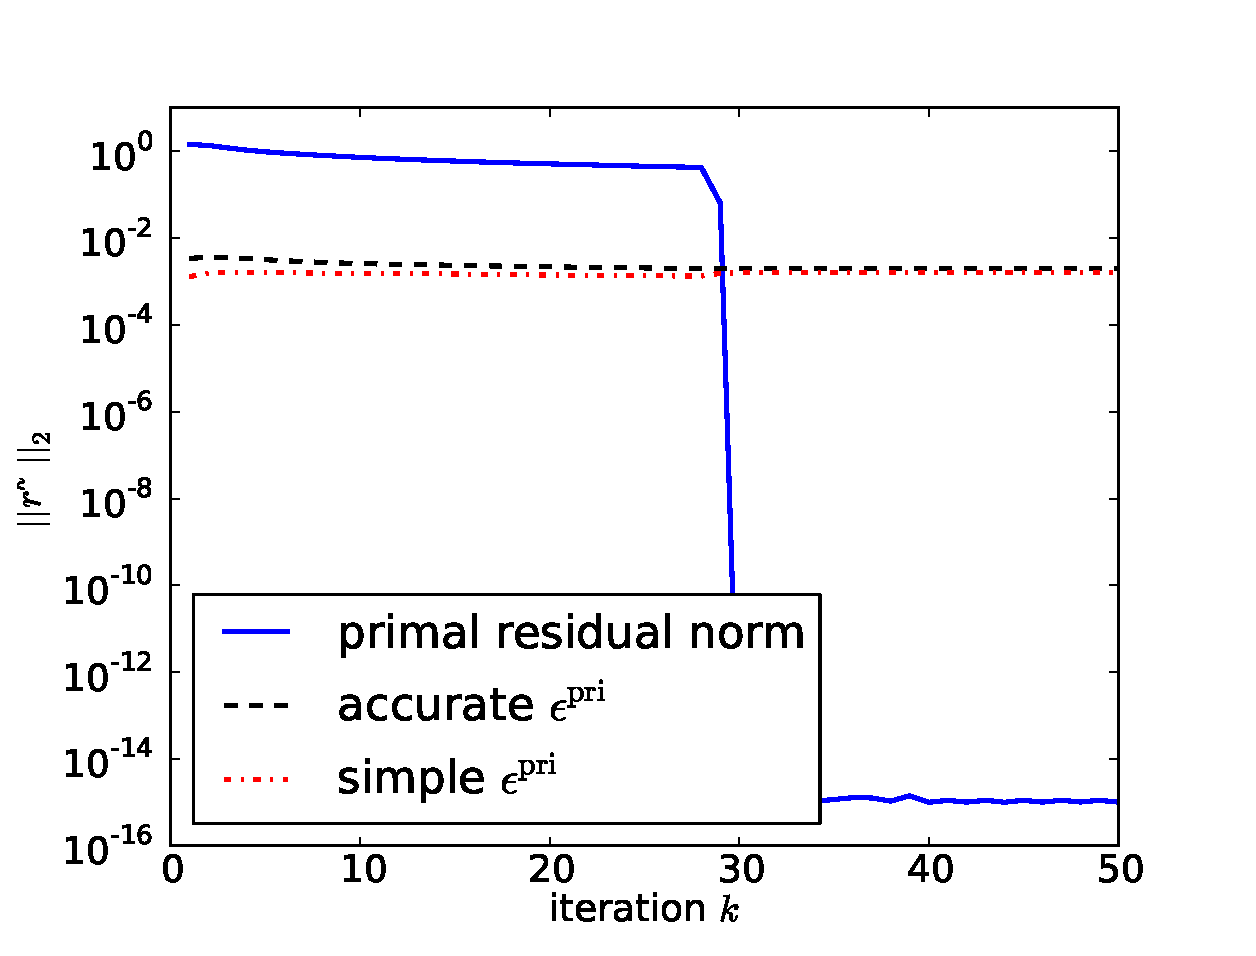
\includegraphics[width=0.49\textwidth]{figures/test_primal_e.eps}
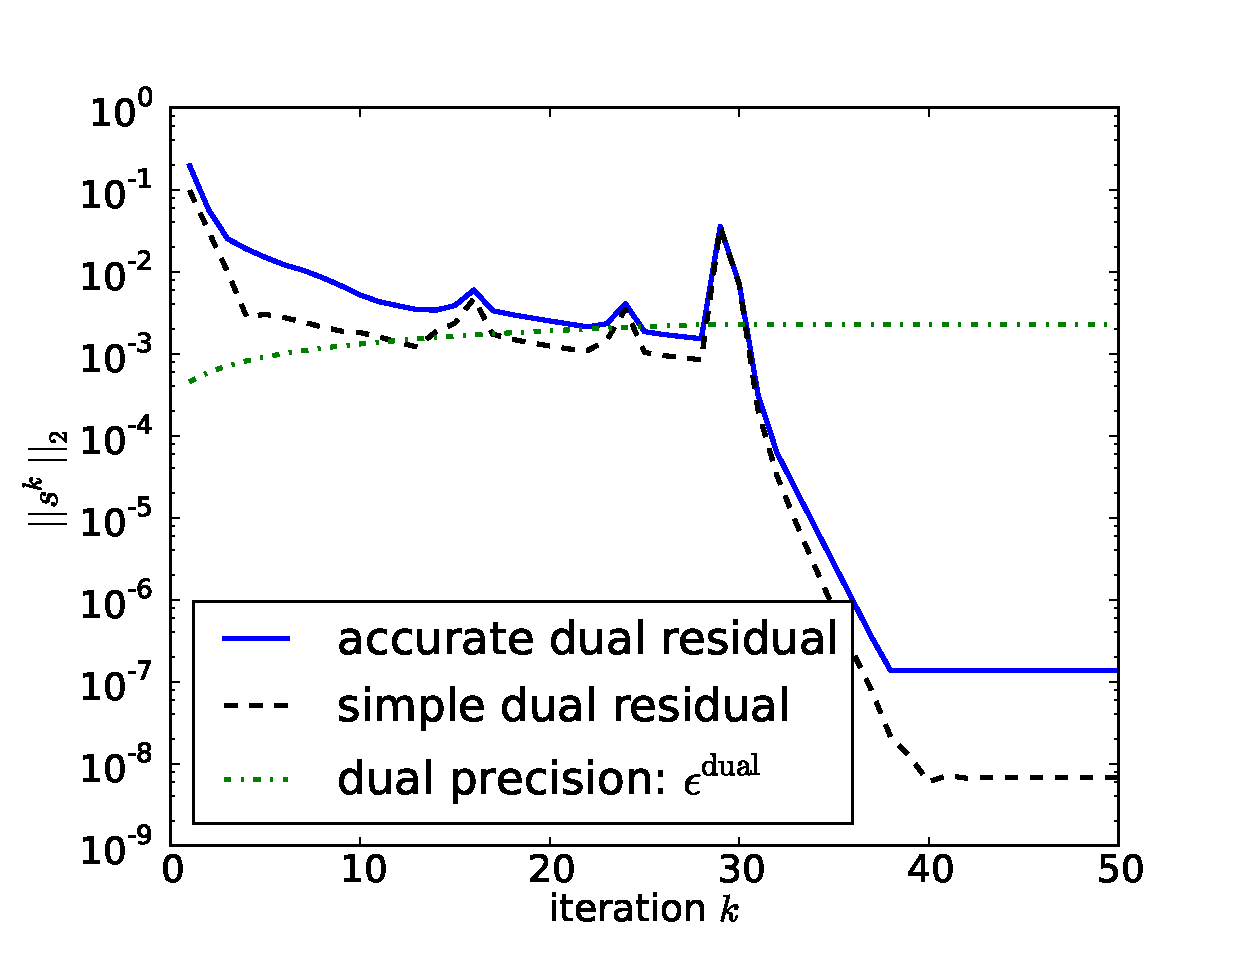
\includegraphics[width=0.49\textwidth]{figures/test_dual_e.eps}
\caption{Progress of reducing primal and dual residual norms in ADMM.
    This is the case of expensive energy, notice that the simple dual
residual often work as well as the accurate dual residual. Since
the resource allocations are not reaching their bounds, so the simple
dual residual $\|s^k\|_2=\rho\|z^{k}-z^{k+1}\|_2$ converges to zero 
only asymptotically, and can serve as a stopping criterion.}
\label{fig:residual-e}
\end{figure}

\begin{figure}[th]
\centering
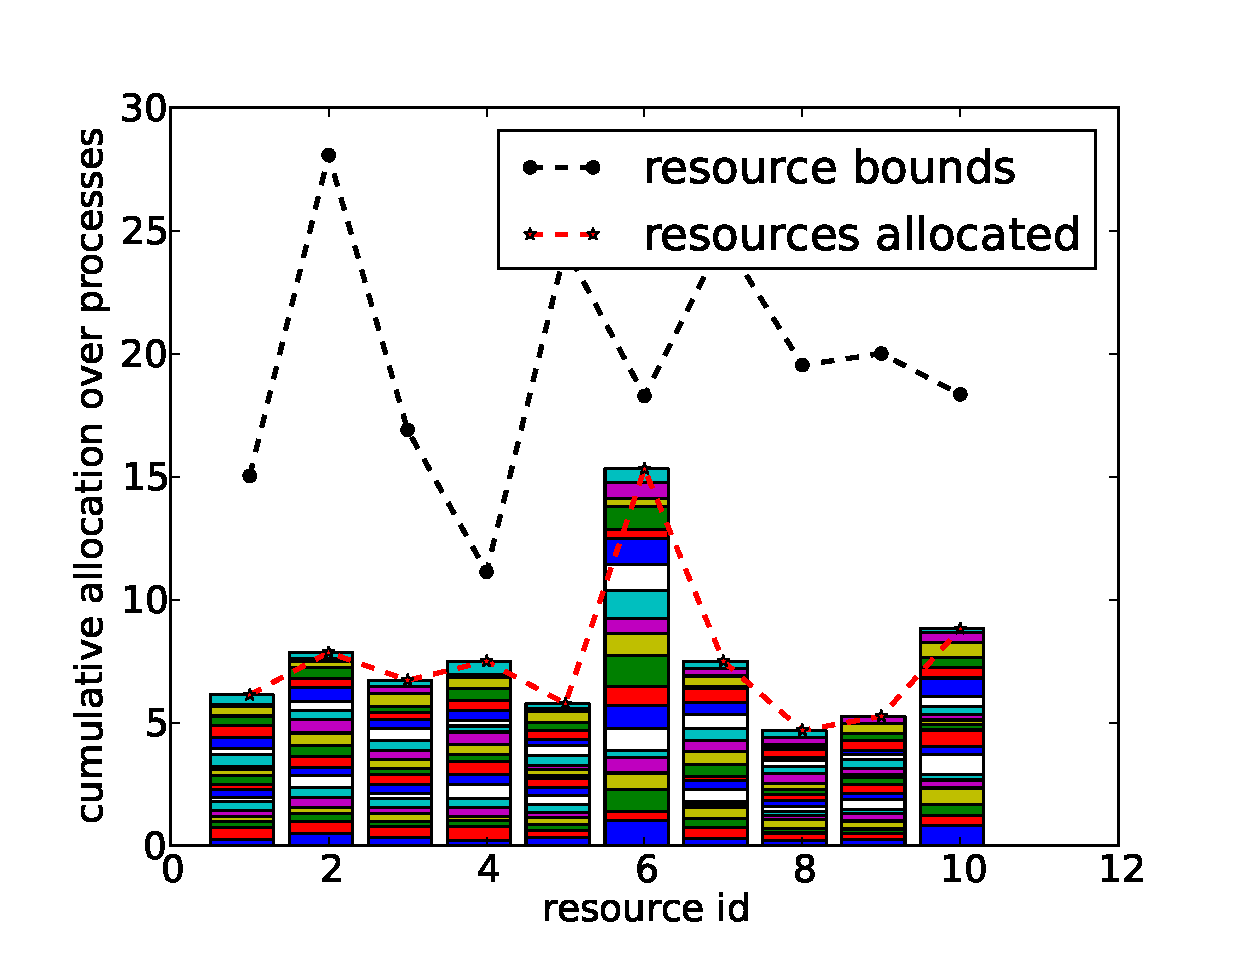
\includegraphics[width=0.49\textwidth]{figures/test_resource_e.eps}
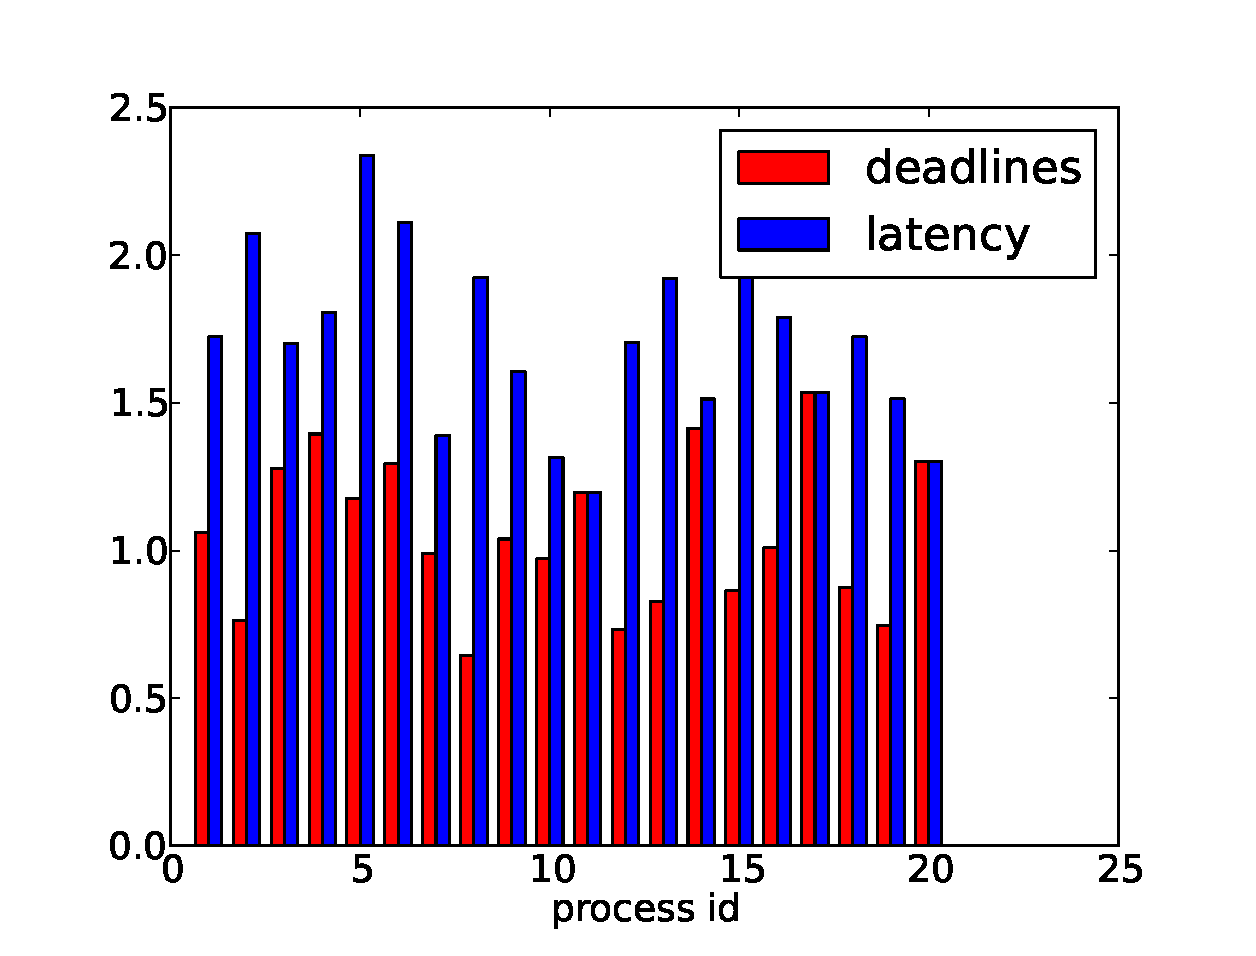
\includegraphics[width=0.49\textwidth]{figures/test_latency_e.eps}
\caption{Visualization of optimal resource allocation (left) and 
    resulting latency for each process (right).
    There are $n=10$ resources and $N=20$ processes.
    This is the case of expensive energy, so the total resouces allocated
    are mostly well below their bounds, but the process latency are mostly
exceeding the deadlines.}
\label{fig:allocation-e}
\end{figure}


\begin{figure}[th]
\centering
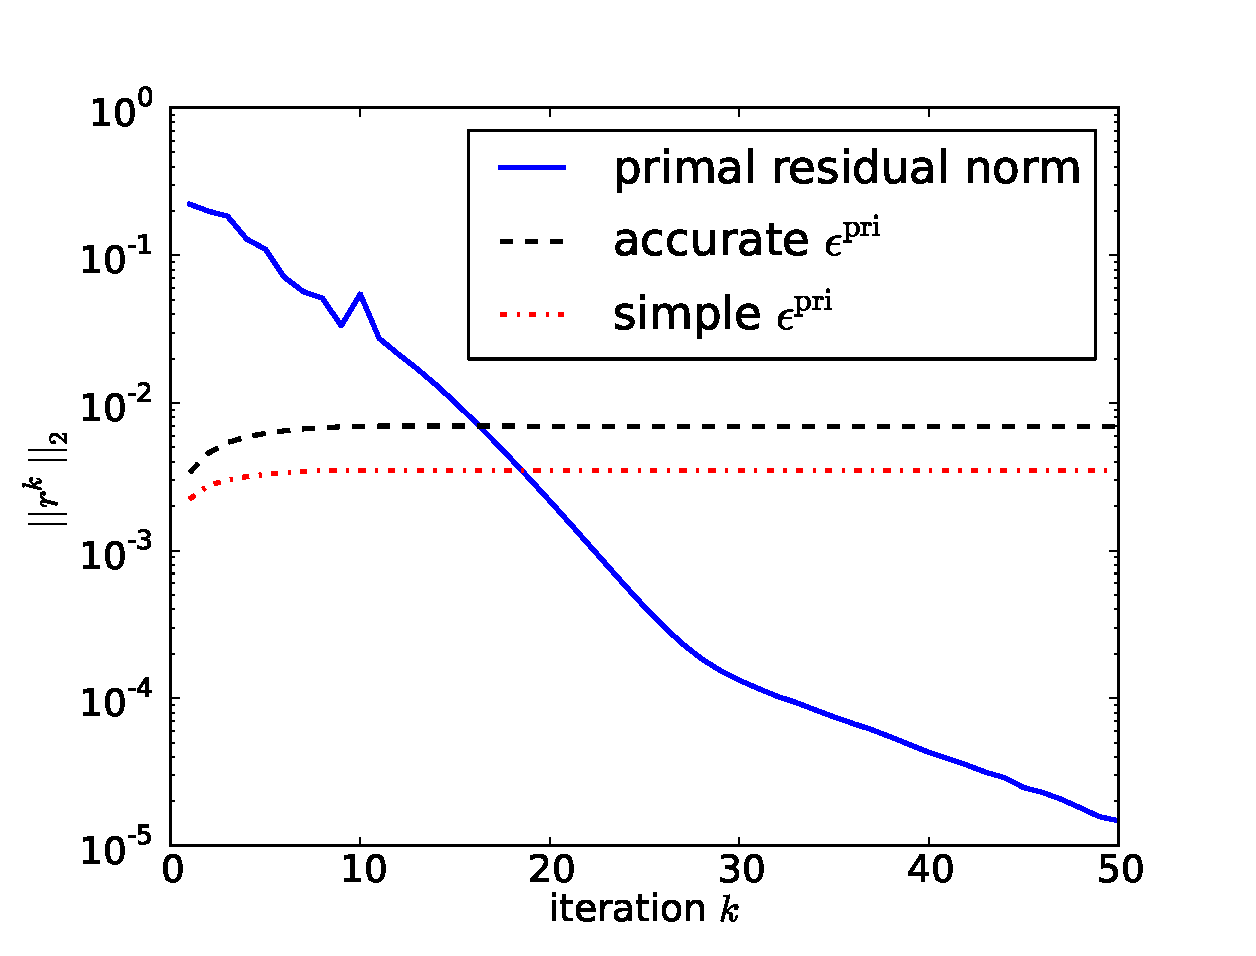
\includegraphics[width=0.49\textwidth]{figures/test_primal_c.eps}
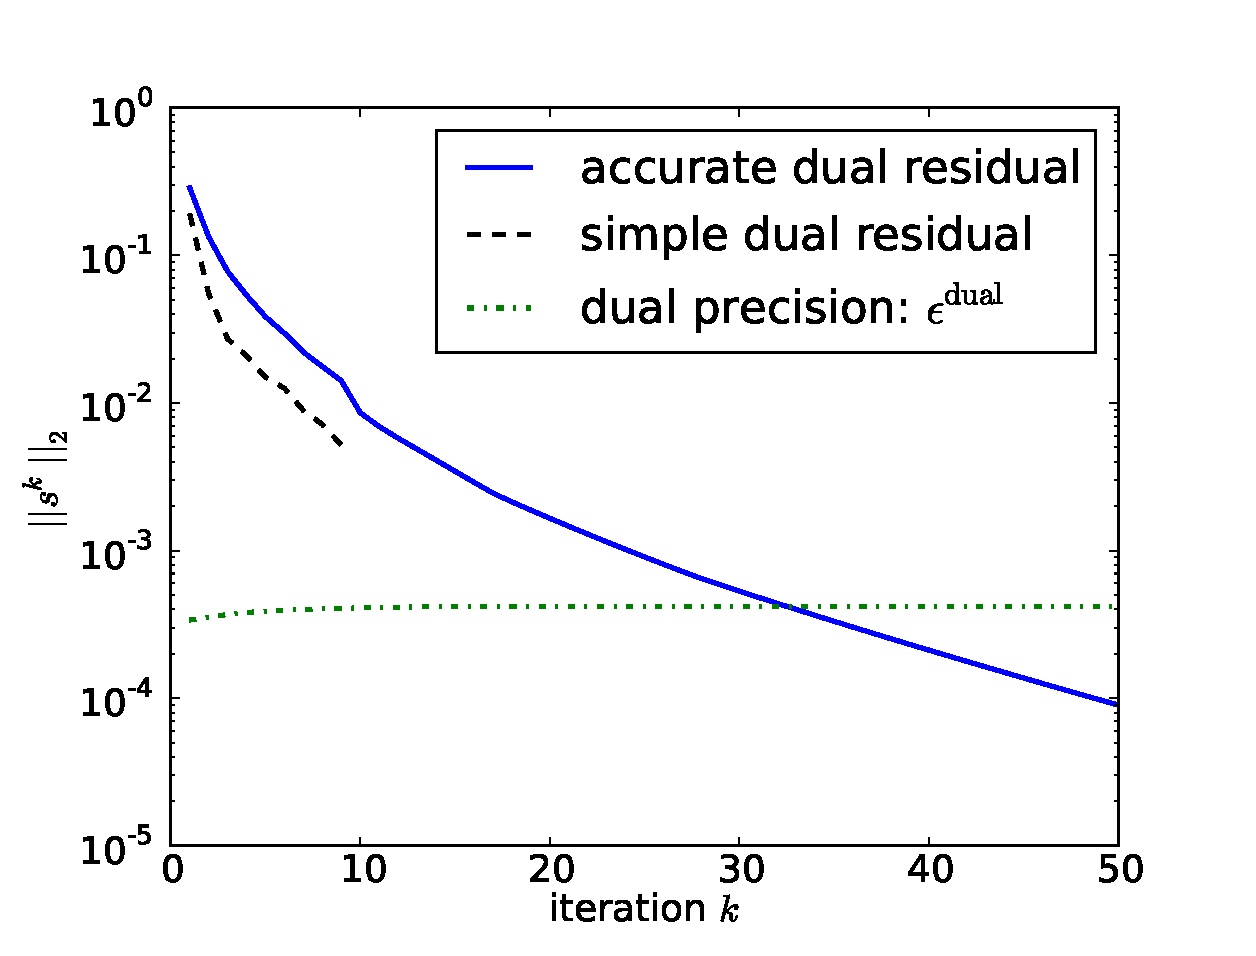
\includegraphics[width=0.49\textwidth]{figures/test_dual_c.eps}
\caption{Progress of reducing primal and dual residual norms in ADMM.
    This is the case of cheap energy, notice that the simple dual
residual becomes exactly zero (discontinued in the plot) after 10 iterations, 
Since the enerygy is cheap, the resource allocations reach their bounds easily,
so the simple dual residual $\|s^k\|_2=\rho\|z^{k}-z^{k+1}\|_2=0$ 
become zero quickly, therefore can \emph{not} serve as a stopping criterion.}
\label{fig:residual-c}
\end{figure}

\begin{figure}[th]
\centering
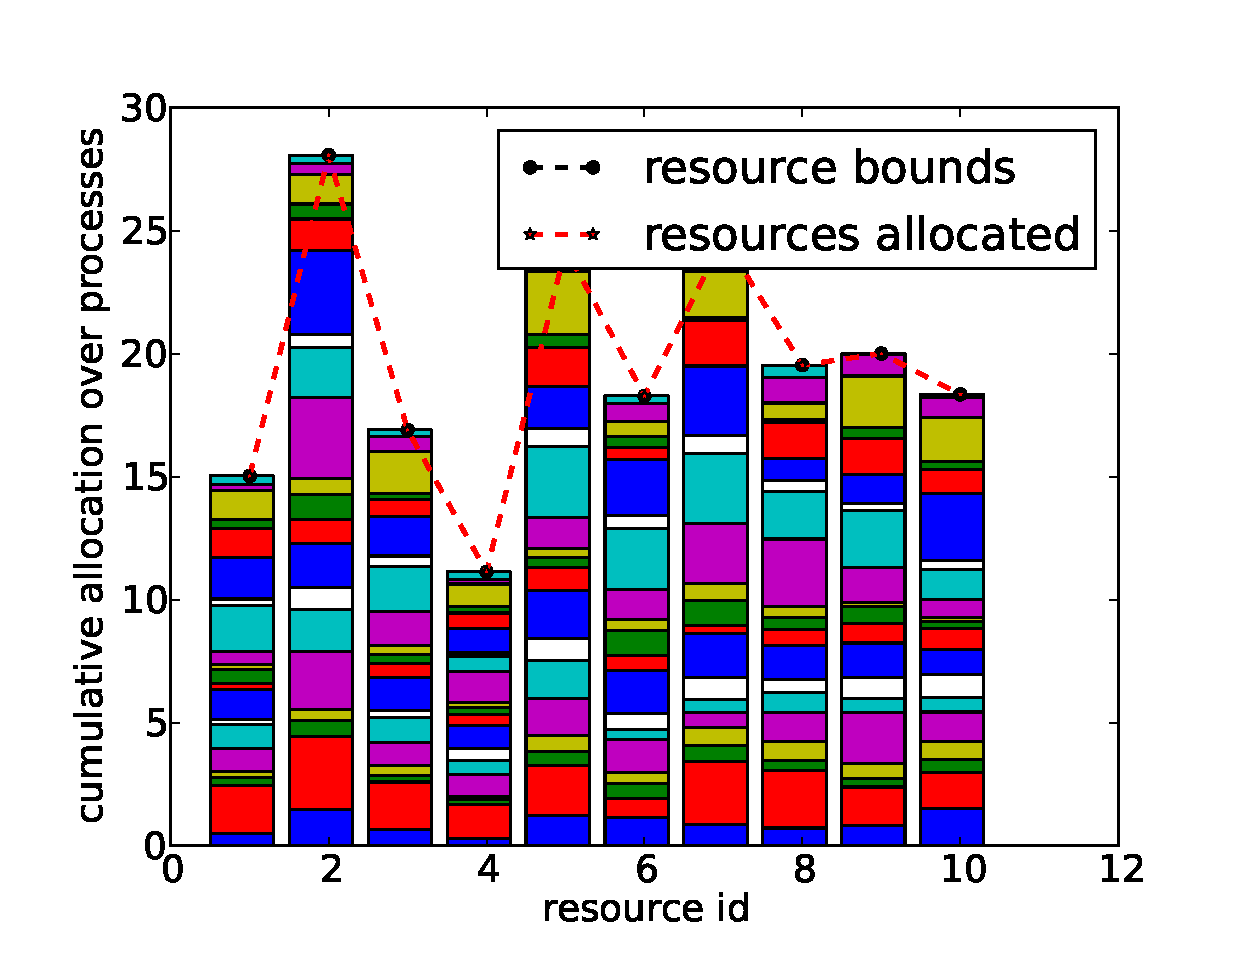
\includegraphics[width=0.49\textwidth]{figures/test_resource_c.eps}
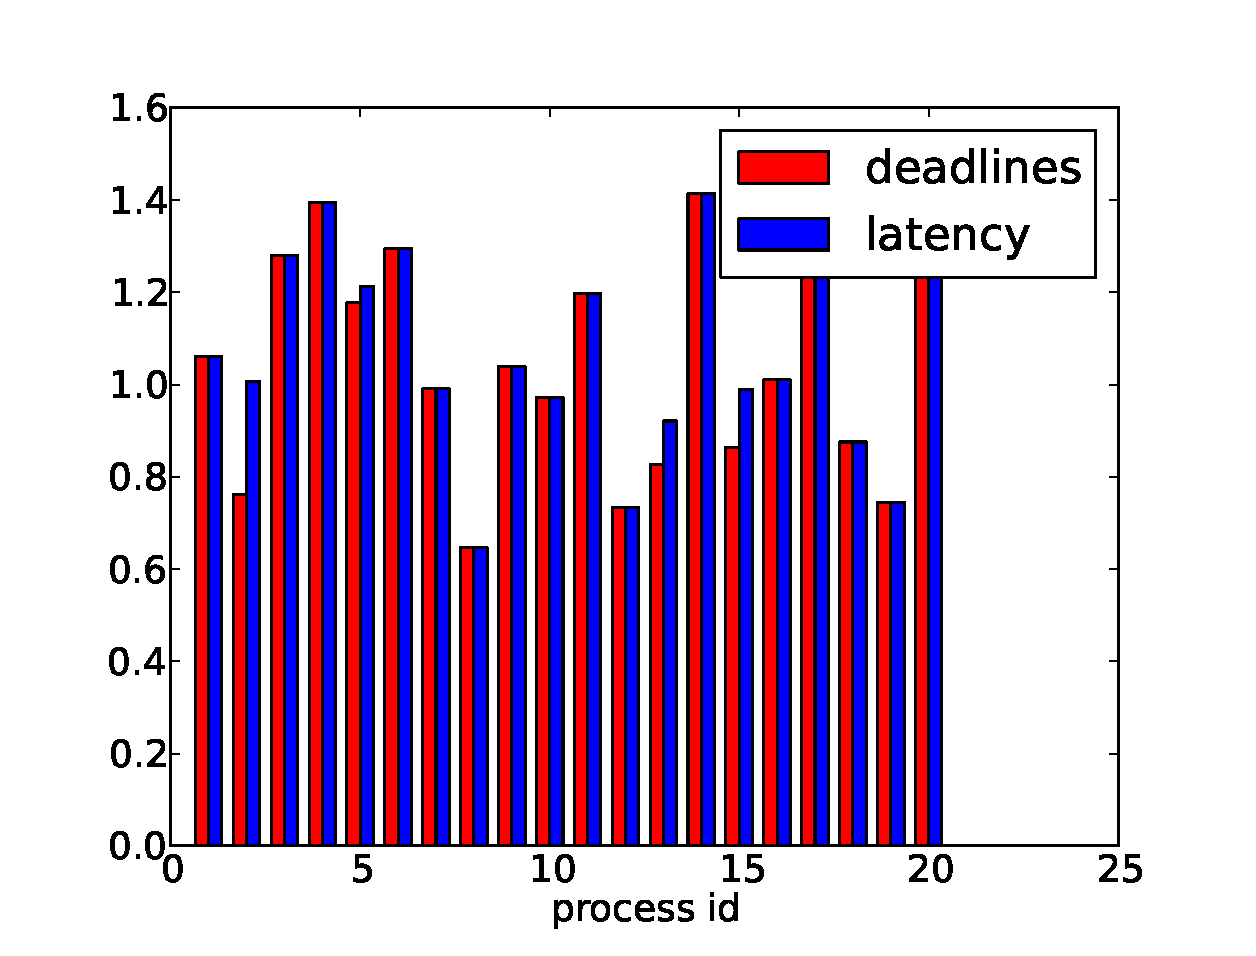
\includegraphics[width=0.49\textwidth]{figures/test_latency_c.eps}
\caption{Visualization of optimal resource allocation (left) and 
    resulting latency for each process (right).
    There are $n=10$ resources and $N=20$ processes.
    This is the case of cheap energy, so the total resouces allocated
    all reach their bounds, and most of the process latency are 
within their deadlines.}
\label{fig:allocation-c}
\end{figure}

\section{Summary}


\chapter{Evaluation and Results}
\section{Dynamic Resource Allocation in a Manycore OS}\label{eval-dynamic}
%	c.	Dynamic System
%		i.	Single Application � right sizing
%			1.	Without phase changes
%			2.	With phase changes
%			3.	Baseline � all allocations
%			4.	Measure Energy
%		ii.	Video, Animation, and Throughput Applications w/o phase changes
%			1.	Show throughput and missed deadlines for all the possible mixes
%			2.	Is it possible to show optimal?
%			3.	What is the baseline?
%		iii.	Video, Animation, and Throughput Applications w/ phase changes
%			1.	Show throughput and missed deadlines for all the possible mixes
%			2.	Basically just to show the system works



\begin{figure*}[!t]
	\begin{center}	
		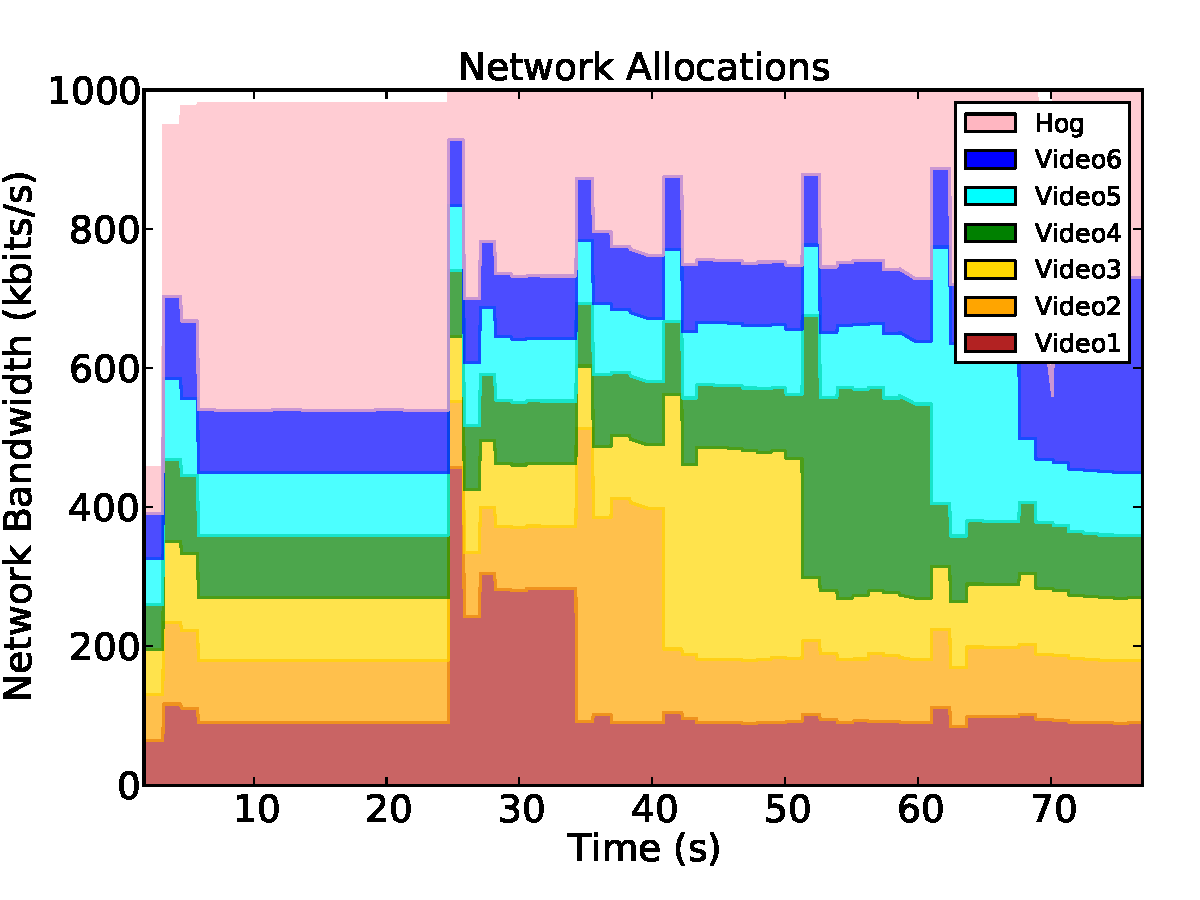
\includegraphics[bb=0 0 576 432,width=.49\textwidth]{Figures/dyn-alloc-wp-ns.pdf}
		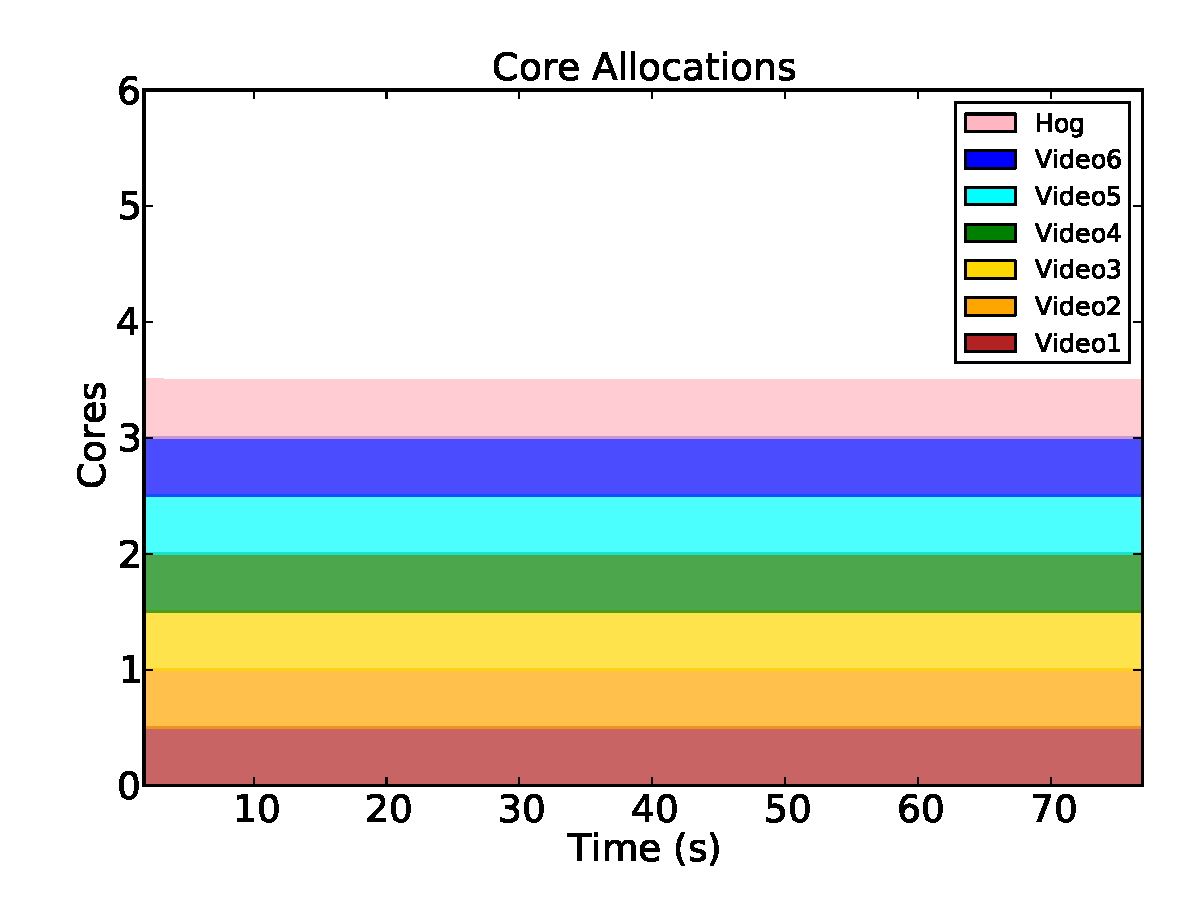
\includegraphics[bb=0 0 576 432,width=.49\textwidth]{Figures/dyn-alloc-wp-core.pdf}
		\caption{Wall Power Mode: Resource Allocations of video conferencing through time as the videos change resolution to adjust for which person is speaking. Hog represents a background task uploading files.}
		\label{video_experiment_wp}
	\end{center}
\end{figure*}

\begin{figure}[!t]
	\begin{center}	
		\includegraphics[bb=0 0 576 432,width=\columnwidth]{Figures/opt_time.pdf}
%		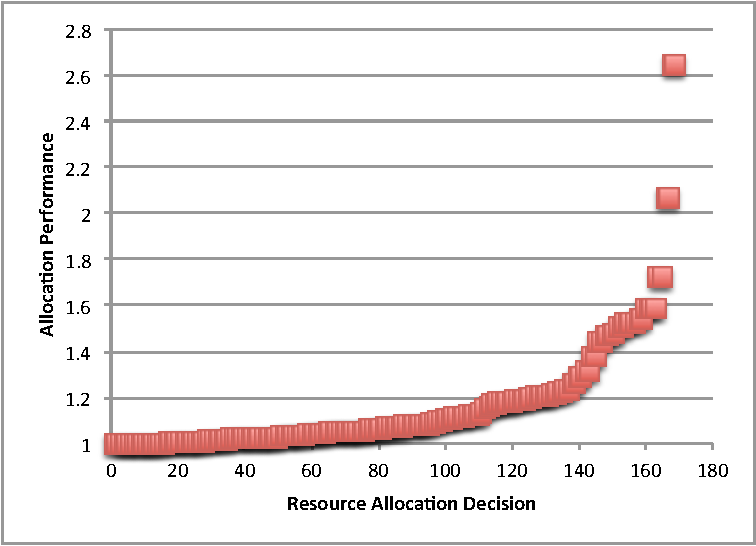
\includegraphics[width=.45\textwidth]{parsec_decision_points.pdf}
		\caption{Performance of our penalty optimization algorithm}
		\label{optimization_perf}
	\end{center}
\end{figure}

\begin{figure}[!t]
	\begin{center}	
		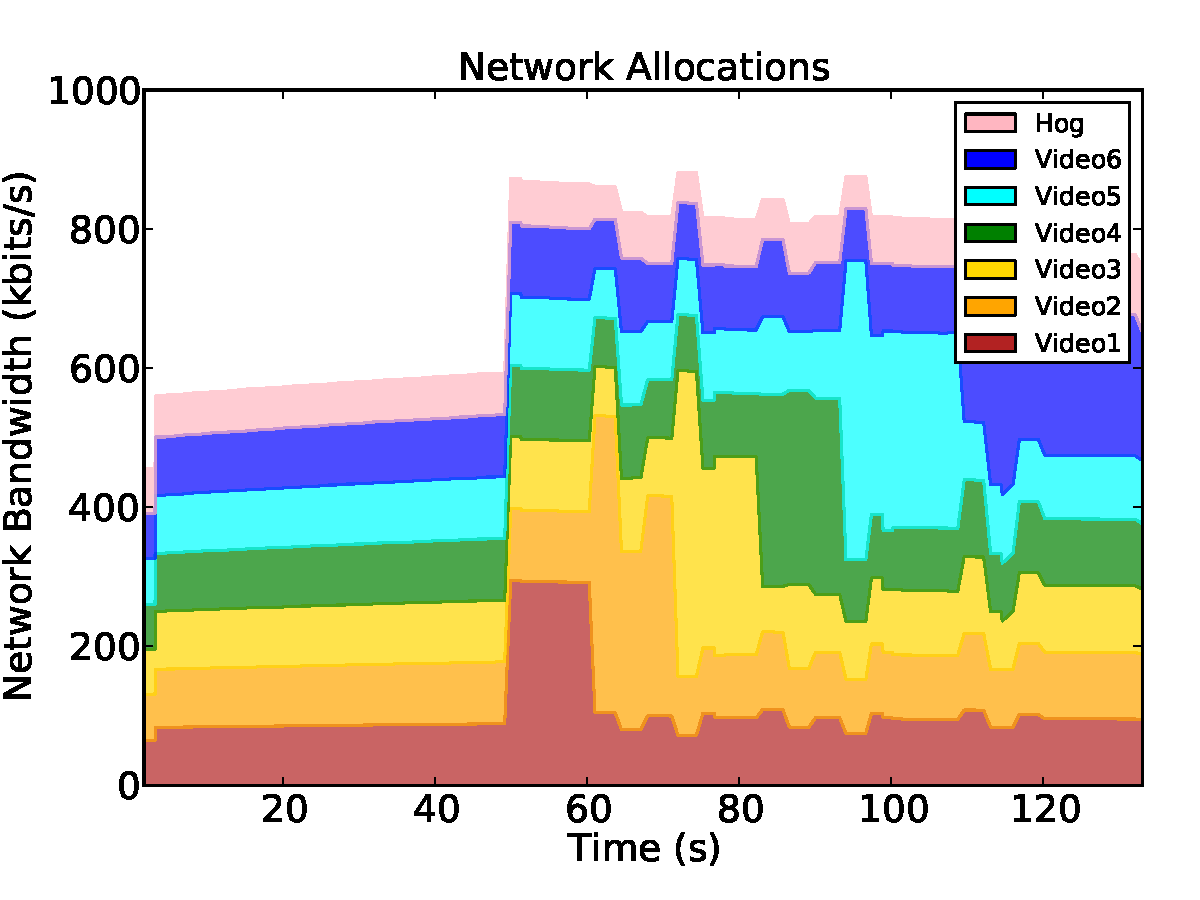
\includegraphics[bb=0 0 576 432,width=\columnwidth]{Figures/dyn-alloc-battery-ns.pdf}
		\caption{Battery Power Mode: Resource Allocations of video conferencing through time as the videos change resolution to adjust for which person is speaking. Hog represents a background task uploading files.}
		\label{video_experiment_battery}
	\end{center}
\end{figure}

%\cite{tess09,tess_dac}

To evaluate \pacora's ability to make real-time decisions in a real operating system, we implemented it in an in-house research operating system, \tess. We chose to implement in \tess rather than Linux for three reasons:
 \begin{enumerate}\itemsep0pt \parskip0pt \parsep5pt
\item \tess separates resource allocation from scheduling, so is
  closer to the OS architecture assumed by \pacora
\item \tess allows resource revocation, enabling \pacora to dynamically reallocate resources
\item \tess implements additional resource partitioning mechanisms,
  letting \pacora manage  more resource types
\end{enumerate}
This dynamic framework is used to test our implementations of the algorithms, measure the overhead and reaction times, and illustrate \pacora's ability to work in a real system.

\subsection{Platform}
Our dynamic experiments are all run on an Intel Nehalem-EP system with two 2.66-GHz Xeon X5550 quad-core processors and hyperthreading enabled with 16 hardware threads. This system also contains a 1-Gbps Intel Pro/1000 Ethernet network adapter.
\tess allocates resources directly to applications, and the applications employ a second-level scheduler to schedule work onto the resources.  
%There are two scheduling frameworks available in \tess: a cooperative framework called Lithe (LIquid THrEads)~\cite{lithe} and a preemptive one called PULSE (Preemptive User-Level SchEduling).  
All of our experiments use a preemptive scheduling framework called PULSE (Preemptive User-Level SchEduling), with two different scheduling strategies: applications with responsiveness requirements use an earliest-deadline-first (EDF) scheduler and throughput-oriented applications use a round-robin (GRR) scheduler.

In addition to allocating cores and cache ways as with our static
framework, \tess can also allocate fractions of network bandwidth.  In
our experiments, we show \pacora allocating cores and network
bandwidth because the experimental platform, which has the advantage
of more cores, does not have cache partitioning.  We have also
successfully experimented with additional resources such as memory pages and CPU
utilization, but the results are not presented here for brevity.

\subsection{Performance and Energy Measurement}

Applications report their own measured response times to \pacora
through a message-passing interface built into \tess, and \pacora uses
this information to build models offline or online.  The online models
are identical to our offline models for the same inputs, so the method
used has no effect on resource allocation decisions.  However, online
models are able to adapt changes in applications.  Modeling is
discussed further in Section~\ref{RTFs}.
%and we also use this information to show if the application is making its deadlines for the experiments.

\tess enables \pacora to directly measure the system energy.  However, energy counters are not available on our Nehalem-EP system and thus we extend the power model from the Sandy Bridge system to function as our application 0 RTF.

\subsection{Description of Workloads}
Our workload is designed to represent a video conference with participants from many remote locations. There is a separate, performance-guaranteed incoming video stream for each participant.
%New participants may join the conference and others may leave, increasing or decreasing the number of streams running at any given time.
The application adjusts video sizes based on which person is
speaking. The speaker's video is larger and has higher resolution than
the other video streams, and as the speaker changes, the requirements
for the video streams change. In the background, network-intensive
tasks such as uploading and downloading files are executed.
%While conferencing, compute-intensive tasks such as virus scans or file indexing could be executed in the background.

Our streaming video application is a multi-threaded, CPU- and
network-intensive workload intended to simulate video chat
applications like Skype and Facetime.  Each video stream is encoded
offline in the H.264 format using libx264, transported across the
network through a TCP connection from a Linux E5-based server, and
decoded and displayed by the \tess client. The client receives,
decodes, and displays each frame using libffmpeg and libx264. Each
video stream has a corresponding EDF-scheduled thread with 33 ms
deadlines using our second-level EDF scheduler.  We also use a network
bandwidth hog application designed to represent an application such as
Google Drive or Dropbox uploading files to the cloud. The hog contends
with the video player for bandwidth by constantly sending UDP messages
to the Linux server.

%We use psearchy~\cite{psearchy}, a parallel text indexer, from MOSBENCH\cite{mosbench} as our file indexing application.



\subsection{Resource Allocation Experiments}

We constrain the available resources in the system for \pacora to 1
Mbit/s network bandwidth and 6 cores to simulate a
resource-constrained system as this is a more challenging resource
allocation problem.

In our experiment the video conference contains 6 incoming video
streams.  At first no one is speaking and thus all the videos are
small.  The person speaking rotates across the incoming videos 1--6,
with the videos resizing around every 10 seconds. We set the deadline
to be 33 ms to represent a frame rate of 30 frames/sec. As this rate,
small videos require 80 to 87 kbits/s depending on the particular
frames. Large videos require 250 to 270 kbits/s.  We assign a moderate
penalty (10.0) for missing the deadline to small videos, and a
significant penalty (50.0) for the large videos.  We assign a small
penalty for the network hog (1.0) with no deadline.

Figure~\ref{video_experiment_wp} shows the resource allocations for our video conference scenario when the computer is using ``wall power''.  We mean wall power to imply that saving power is less critical and thus we assign a low penalty slope to application 0.  \pacora gives 90 kbits/s to small videos, 280 kbit/s to large videos, and the remaining bandwidth is given to the network hog.  Video resizes can be seen as the ``steps'' in the graph: for example, Video1 becomes large at 24 seconds resulting in its allocation increasing from 90 kbits/s to 280 kbits/s.  Video2 becomes large at 33 seconds and Video1 returns to its original size.

Since there is a single set of extreme points in a convex problem
after a sufficient number of iterations, our dynamic algorithm will
produce the same allocations as our static framework. The runtime is
controllable based on the exit conditions of the optimization
algorithm, however earlier exits may result in intermediate
reallocations. We can see intermediate resource allocations (the
``columns'' in the graph) as \pacora transitions for one set of
allocations to another.  If run much longer (50 ms), \pacora can
completely eliminate the intermediate allocations, which may be
appropriate in environments where resource reallocation is expensive
and allocations do not need to be adapted frequently.  It is also
possible to provide guaranteed optimization times of around \SI{20}{
\micro\second}, but at the cost of many more intermediate reallocations.
These results can be found in~\cite{pacora_tr}.We choose this
particular point in the space because we believed it strikes the right
balance between reactivity and reallocation amounts for a client
operating system. Figure~\ref{optimization_perf} shows the runtime of
the optimization algorithm as it makes resource allocation decisions
for the video scenario. The algorithm runs in \SI{50}{\micro\second} on average,
with more significant reallocations taking from 250-\SI{350}{\micro\second}.
Significant changes result in 1-2 intermediate reallocations.  In
\tess, network bandwidth is easily reallocated and thus intermediate
reallocations do not have much overhead.  Core allocations are also
easily adjusted between fractional core amounts.  Careful tuning of
the algorithm parameters could potentially yield additional
performance improvements.

Core allocations are also shown in Figure~\ref{video_experiment_wp}.
Neither application in our scenario can take advantage of additional
compute power thus each optimization results in the same core
allocations for the applications regardless of video size.

Figure~\ref{video_experiment_battery} shows same scenario except the
computer is now using ``battery power'' and thus we have increased the
importance of application 0 (penalty 2.0).  The video applications are
still allocated the necessary amount of resources for each video size.
However, the allocation of the network hog is significantly reduced to
less than 70 kbits/s, and the remaining resources are left idle.




\chapter{Discussion}\label{discuss}

don't forget to discuss, averaging response times, modifying applications, measuring heartbeats, inferring penalty or deadlines

There are two main sources of challenges for \pacora's design: performance non-convexity and performance variability.  In the following section we describe possible techniques for coping with these challenges.

The main concern with performance non-convexity and variability is their effects on the accuracy of the response time functions.  However, an important result we have found while evaluating \pacora is that model accuracy has less impact on the quality of resource allocation decisions than we anticipated.  When experimenting with possible models for the RTFs, we found that while some models were always a little too inaccurate and did degrade the performance of the resource allocation decisions, once a model crossed a certain threshold of accuracy then better models provided insignificant improvement in resource allocation decisions.  Although there is a slight correlation between model accuracy and decision quality, many decisions with inaccurate models still result in near optimal allocations.  This effect enables \pacora's model-based design to be feasible in a noisy system with real applications.

\section{Outliers and Performance Non-Convexity}

Outliers and performance non-convexity can be handled with a combination of two techniques.  Outliers should be thrown out during the model creation phase as described in Section~\ref{RTFs} to prevent those points from distorting the accuracy of the other allocations.  The second part of the solution is to keep track of these points with extreme error in the model and use heuristics to adjust the resource allocations to avoid such points.  We did not implement this second idea in our current evaluation, but it is a subject of future study.  In our study, we experienced outliers for a few applications with a particular number of hyperthreads and for many applications when given only one cache way. However, as responsiveness, predictability, and efficiency increase in importance for systems, we expect to see an increased number of chip designs that provide more performance convexity.

\section{Variability}

We observe three main sources of variability in application performance: phase changes, performance changes due to differing inputs, and variable resource performance due to external causes or interference from sharing.

\section*{Phases}
As described in Section~\ref{RTFs}, phases can be handled with online creation of the RTFs.  However, another option is to build different models, one per phase, and swap models when a change occurs.  We used this method for the video application in Section~\ref{eval-dynamic}.  This approach has the advantage that it can more rapidly adapt to phases; however it requires identifying phases and additional space to store the extra models. Phase detection is an active area of research, and \cite{dhodapkar-micro03} provides an overview of techniques.  Another possible approach is to build a model that represents the resource requirements of the most demanding phase.  The system can be designed make use of the idle resources when available or power management mechanisms can put them in low-power mode.

\section*{Input Dependence}
Some applications may significantly change performance as a function of their inputs. In the case of our video application we ignored its input dependence without significant effect.  However for other applications the effect may be more pronounced. As with phases, a solution might be to keep multiple models for the application and select one based on the current input.  A different solution is to make the RTFs \emph{stochastic models} representing the distribution of response times of the application.  Stochastic models for \pacora are discussed in more detail in~\cite{pacora_tr}.

\section*{Resource Variability}
In our study we experience resource variability both in the form of non-deterministic resources such as the network connection in \texttt{ tradebeans} or dynamic frequency changes in the CPU and shared resources such as memory bandwidth. Stochastic models are most likely the right way to deal with non-deterministic resources and may be particularly necessary for representing disk-based storage in warehouse scale computing.

Shared resources can also be handled with stochastic models.  However, since the models can be built online while other applications are running, the interference from a loaded machine is already captured in the model.  In our evaluation of static allocation, we built the models in isolation but found that \pacora was still able to make near-optimal resource allocations for a loaded machine despite the shared resources.

While there will likely always be some shared resources, we have found
a trend towards minimizing interference in emerging chip designs, as
efficiency and predictability begin to trump utilization as primary
concerns.


%other types of non-deterministic apps?



% don't forget cpu frequency

%------------------------------------------------------------------------------------------------------------------------------------------------------------------------
\section{Possible RTF Extensions}
%------------------------------------------------------------------------------------------------------------------------------------------------------------------------
\subsection{Alternative Resource Representations}
Asynchrony and latency tolerance may make response time components overlap partly or fully;
if the latter, then the maximum of the terms might be more appropriate than their sum.
The result will still be convex, though, as will any other norm including the 2-norm,
\emph{i.e.} the square root of the sum of the squares.
This last variation could be viewed as a ``partially overlapped'' compromise between
the 1-norm (sum) describing no overlap and the $\infty$-norm (maximum) describing full overlap.

Sometimes a response time component might be better modeled by a term involving a combination of resources.
For example, response time due to memory accesses might be approximated
by a combination of memory bandwidth allocation $b_{r1}$ and cache allocation $m_{r2}$.
Such a model could use the geometric mean of the two allocations in the denominator,
\emph{viz.} $w_{r1,r2}/\sqrt{b_{r1}\cdot m_{r2}}$, without compromising convexity.

This scheme also accommodates non-bandwidth resources such as memory,
the general idea being to roughly approximate ``diminishing returns'' in the response time with increasing resources.
For clarity's sake, rather than using $a_r$ indiscriminately for all allocations,
we will denote an allocation of a bandwidth resource by $b_r$ and of a memory resource by $m_r$.
This begs the question of how memory affects the response time.
The effect is largely indirect.
Memory permits exploitation of temporal locality and thereby \emph{amplifies} associated bandwidths.
For example, additional main memory may reduce the need for storage or network bandwidth,
and of course increased cache capacity may reduce the need for memory bandwidth.
The effectiveness of cache in reducing bandwidth was studied by
H. T. Kung\cite{Kung}, who developed tight asymptotic bounds on the bandwidth amplification
factor $\alpha(m)$ resulting from a quantity of memory $m$ acting as cache for a variety of computations.
He shows that
\begin{displaymath}
\begin{array}{lll}
\alpha(m) &= \Theta(\sqrt m) & \mbox{for dense linear algebra solvers} \\
          &= \Theta(m^{1/d}) & \mbox{for d-dimensional PDE solvers} \\
          &= \Theta(\log m)  & \mbox{for comparison sorting and FFTs} \\
          &= \Theta(1)       & \mbox{when temporal locality is absent}
\end{array}
\end{displaymath}

For these expressions to make sense, the argument of $\alpha$ should be dimensionless and greater than 1.
Ensuring this might be as simple as letting it be the number of memory resource quanta
(\emph{e.g.} hundreds of memory pages) assigned to the application.
If a application shows diminishing bandwidth amplification as its memory allocation increases, this can be accommodated:
\begin{displaymath}
\alpha(m) = \min(c_1\alpha_1(m),c_2\alpha_2(m)),\;c_1,c_2 \geq 0
\end{displaymath}

Each bandwidth amplification factor might be described by one of the functions above
and included in the denominator of the appropriate component in the response time function model.
For example, the storage response time component for the model of an out-of-core sort application might be
the quantity of storage accesses divided by the product of the storage bandwidth allocation and $\log m$,
the amplification function associated with sorting given a memory allocation of $m$.
Amplification functions for each application might be learned from response time measurements
by observing the effect of varying the associated memory resource while keeping the bandwidth allocation constant.
Alternatively, redundant components, similar except for amplification function, could be included in the model
to let the model fitting process decide among them.

\subsection{Stochastic Models}
Execution times are random to some extent. Variations in amounts of work within an application are reflected only after the fact by the $w_i$ which change as the process runs.  Insufficiently isolated resources may also cause such variability. Complicating things further, service objectives may specify guarantees in the form of high probability upper bounds on actual application runtimes.  The predicted runtimes $\tau$ in these cases are insufficient.
Random fluctuations will be reflected in the runtime measurements t and the residual error $\epsilon = t - \sigma$. The sample mean and standard deviation of the error can bound the probability that the actual runtime will exceed the prediction $\tau$. Using this information, a Chebyshev bound on the error of the form
\begin{equation}
Pr\left\{\left|\frac{(\epsilon-\overline{\epsilon})}{\sigma_\epsilon}\right| > k\right\}\leq\frac{1}{k^2} 
\end{equation}
can guarantee the probability that a particular runtime requirement is met.
For example, a runtime upper bound of 50 microseconds with probability 0.99, given an error sample mean of 3 microseconds (meaning $\tau$ underestimates t by that much) and a sample standard deviation of 2 microseconds, leads to the requirement that $\tau + 3$ must be less than $50 - k \sigma\epsilon = 50 - 10\times2 = 30$ microseconds to guarantee that $t = \tau  + \epsilon$ exceeds 50 microseconds only 1\% of the time.  The penalty function deadline for this application should accordingly be set to 27 microseconds.  Of course if the system is incapable of meeting all of its deadlines, penalty slopes will determine the extent of the violations.




\subsection{Handling Quasiconvex Response Time Functions}

There are examples of response time versus resource behavior that violate convexity.  One such example sometimes occurs in memory allocation, where ``plateaus'' can sometimes be seen as in Figure~\ref{f:plat}.

Such plateaus are typically caused by algorithm adaptations within the application to accommodate variable resource availability.  The response time is really the \emph{minimum} of several convex functions depending on allocation and the point-wise minimum that the application implements fails to preserve convexity.  The effect of the plateaus will be a non-convex penalty as shown in Figure~\ref{f:plateffect} and multiple extrema in the optimization problem will be a likely result.

There are several ways to avoid this problem.  One is based on the observation that such response time functions
will at least be \emph{quasiconvex}.  A function $f$ is quasiconvex if all of its \emph{sublevel sets}
$S_\ell = \{x | f(x) \leq \ell\}$ are convex sets.
Alternatively, $f$ is quasiconvex if its domain is convex and
\begin{displaymath}
f(\theta x + (1-\theta)y) \leq \max(f(x),f(y)), 0 \leq \theta \leq 1
\end{displaymath}

Quasiconvex optimization can be performed by selecting a threshold $\ell$ and replacing the objective function
with a convex constraint function whose sublevel set $S_\ell$ is the same as that of $f$.
Next, one determines whether there is a feasible solution for that particular threshold $\ell$.
Repeated application with a binary search on $\ell$ will reduce the level of feasibility
until the solution is approximated well enough.

Another idea is to use additional constraints to explore convex sub-domains of $\tau$.
For example,the affine constraint $a_{p,r} - \mu \leq 0$ excludes application $p$ from any assignment of resource $r$ exceeding $\mu$.  Similarly, $\mu - a_{p,r} \leq 0$ excludes the opposite possibility.
A binary (or even linear)search of such sub-domains could be used to find the optimal value.


\subsection{Heterogeneity}

Heterogeneity is naturally handled by \pacora.  Each core type can be viewed as a different resource system, so fat cores may be resource 1, thin cores may be resource 2, and GPUs could be resource 3.  The application developer would not need to specify, which core types the application uses best; \pacora would try allocating the cores and the resulting performance would be captured in the RTFs.  So, for example, if an application did not use a GPU then this would be discovered empirically and the RTF would show no performance improvement along the GPU dimension.  










\chapter{Conclusion and Future Work}
\pacora takes a different approach to resource allocation than traditional systems, relying heavily on application-specific functions built through measurement and convex optimization.  Using convex optimization lets \pacora perform real-time resource allocation inexpensively, enabling \pacora to dynamically allocate resources to adjust to the changing state of the the system.  \pacora makes resource allocation decisions in less than \SI{350}{\micro\second} in the worst case and often faster than \SI{50}{\micro\second} in our manycore OS implementation. By building application-specific functions online and formulating resource allocation as an optimization problem, \pacora is able to accomplish multi-dimensional resource allocation on a general set of resources, thereby handling heterogeneity and the growing diversity of modern hardware while protecting application developers from needing to understand resources. Allocation decisions are near optimal---only 2\% from the best possible allocation on average, and \pacora only requires a few hundred bytes of additional storage per application.

% \appendix
% \chapter{More Monticello Candidates}

\printbibliography

\end{document}
